\documentclass{report}
\usepackage[spanish]{babel}
\addto\captionsspanish{
  \renewcommand{\contentsname}%
    {Índice}%
}

%%%%%%%%%%%%%%%%%%%%%%%%%%%%%%%%%
% PACKAGE IMPORTS
%%%%%%%%%%%%%%%%%%%%%%%%%%%%%%%%%


\usepackage[tmargin=2cm,rmargin=1in,lmargin=1in,margin=0.85in,bmargin=2cm,footskip=.2in]{geometry}
\usepackage{amsmath,amsfonts,amsthm,amssymb,mathtools}
\usepackage{wrapfig}
\usepackage{subcaption}
\usepackage{afterpage}
\usepackage[varbb]{newpxmath}
\usepackage{xfrac}
\usepackage[T1]{fontenc}
\usepackage{tabularx}
\usepackage{floatrow}
\usepackage{enumerate}
\newfloatcommand{capbtabbox}{table}[][\FBwidth]
\usepackage{amssymb}
%command for alg-closure that automatically adapts its 'bar' to the arg based on the args length (including '\')
\newcommand{\ols}[1]{\mskip.5\thinmuskip\overline{\mskip-.5\thinmuskip {#1} \mskip-.5\thinmuskip}\mskip.5\thinmuskip} % overline short
\newcommand{\olsi}[1]{\,\overline{\!{#1}}} % overline short italic
\makeatletter
\newcommand\ovl[1]{
  \tctestifnum{\count@stringtoks{#1}>1} %checks if number of chars in arg > 1 (including '\')
  {\ols{#1}} %if arg is longer than just one char, e.g. \mathbb{Q}, \mathbb{F},...
  {\olsi{#1}} %if arg is just one char, e.g. K, L,...
}
% FROM TOKCYCLE:
\long\def\count@stringtoks#1{\tc@earg\count@toks{\string#1}}
\long\def\count@toks#1{\the\numexpr-1\count@@toks#1.\tc@endcnt}
\long\def\count@@toks#1#2\tc@endcnt{+1\tc@ifempty{#2}{\relax}{\count@@toks#2\tc@endcnt}}
\def\tc@ifempty#1{\tc@testxifx{\expandafter\relax\detokenize{#1}\relax}}
\long\def\tc@earg#1#2{\expandafter#1\expandafter{#2}}
\long\def\tctestifnum#1{\tctestifcon{\ifnum#1\relax}}
\long\def\tctestifcon#1{#1\expandafter\tc@exfirst\else\expandafter\tc@exsecond\fi}
\long\def\tc@testxifx{\tc@earg\tctestifx}
\long\def\tctestifx#1{\tctestifcon{\ifx#1}}
\long\def\tc@exfirst#1#2{#1}
\long\def\tc@exsecond#1#2{#2}
\makeatother
\usepackage[makeroom]{cancel}
\usepackage{mathtools}
\usepackage{bookmark}
\usepackage{enumitem}
\usepackage{hyperref,theoremref}
\hypersetup{
	pdftitle={Apuntes de Análisis de Varias Variables 2},
	colorlinks=true, linkcolor=doc!90,
	bookmarksnumbered=true,
	bookmarksopen=true
}
\usepackage[most,many,breakable]{tcolorbox}
\usepackage{xcolor}
\usepackage{varwidth}
\usepackage{varwidth}
\usepackage{etoolbox}
%\usepackage{authblk}
\usepackage{nameref}
\usepackage{multicol,array}
\usepackage{tikz-cd}
\usepackage[ruled,vlined,linesnumbered]{algorithm2e}
\usepackage{comment} % enables the use of multi-line comments (\ifx \fi) 
\usepackage{import}
\usepackage{xifthen}
\usepackage{pdfpages}
\usepackage{transparent}
\usepackage{titlesec}
\titleformat{\section}{\normalfont\fontsize{17.28pt}{12pt}\selectfont\bfseries}{\thesection}{1em}{}
\usepackage{empheq} % boxed align


\newcommand\mycommfont[1]{\footnotesize\ttfamily\textcolor{blue}{#1}}
\SetCommentSty{mycommfont}
\newcommand{\incfig}[1]{%
    \def\svgwidth{\columnwidth}
    \import{./figures/}{#1.pdf_tex}
}

\newcommand{\notimplies}{\;\not\!\!\!\implies}

\usepackage{tikzsymbols}
\renewcommand\qedsymbol{$\Laughey$}

\newcommand\phantomarrow[2]{%
  \setbox0=\hbox{$\displaystyle #1\to$}%
  \hbox to \wd0{%
    $#2\mapstochar
     \cleaders\hbox{$\mkern-1mu\relbar\mkern-3mu$}\hfill
     \mkern-7mu\rightarrow$}%
  \,}

%\usepackage{import}
%\usepackage{xifthen}
%\usepackage{pdfpages}
%\usepackage{transparent}


%%%%%%%%%%%%%%%%%%%%%%%%%%%%%%
% SELF MADE COLORS
%%%%%%%%%%%%%%%%%%%%%%%%%%%%%%



\definecolor{myg}{RGB}{56, 140, 70}
\definecolor{myb}{RGB}{45, 111, 177}
\definecolor{myr}{RGB}{199, 68, 64}
\definecolor{mytheorembg}{HTML}{f5e4e1}
\definecolor{mytheoremfr}{HTML}{7B0000}
\definecolor{mylenmabg}{HTML}{FFFAF8}
\definecolor{mylenmafr}{HTML}{983b0f}
\definecolor{mypropbg}{HTML}{f2fbfc}
\definecolor{mypropfr}{HTML}{191971}
\definecolor{myexamplebg}{HTML}{F2FBF8}
\definecolor{myexamplefr}{HTML}{88D6D1}
\definecolor{myexampleti}{HTML}{2A7F7F}
\definecolor{mydefinitbg}{HTML}{E5E5FF}
\definecolor{mydefinitfr}{HTML}{3F3FA3}
\definecolor{notesgreen}{RGB}{0,162,0}
\definecolor{myp}{RGB}{197, 92, 212}
\definecolor{mygr}{HTML}{2C3338}
\definecolor{myred}{RGB}{127,0,0}
\definecolor{myyellow}{RGB}{169,121,69}
\definecolor{myexercisebg}{HTML}{F2FBF8}
\definecolor{myexercisefg}{HTML}{2A7F7F}


%%%%%%%%%%%%%%%%%%%%%%%%%%%%
% TCOLORBOX SETUPS
%%%%%%%%%%%%%%%%%%%%%%%%%%%%

\setlength{\parindent}{1cm}
%================================
% THEOREM BOX
%================================

\tcbuselibrary{theorems,skins,hooks}
\newtcbtheorem[number within=section]{Theorem}{Teorema}
{%
	enhanced,
	breakable,
	colback = mytheorembg,
	frame hidden,
	boxrule = 0sp,
	borderline west = {2pt}{0pt}{mytheoremfr},
	sharp corners,
	detach title,
	before upper = \tcbtitle\par\smallskip,
	coltitle = mytheoremfr,
	fonttitle = \bfseries\sffamily,
	description font = \mdseries,
	separator sign none,
	segmentation style={solid, mytheoremfr},
}
{th}

\tcbuselibrary{theorems,skins,hooks}
\newtcbtheorem[number within=chapter]{theorem}{Teorema}
{%
	enhanced,
	breakable,
	colback = mytheorembg,
	frame hidden,
	boxrule = 0sp,
	borderline west = {2pt}{0pt}{mytheoremfr},
	sharp corners,
	detach title,
	before upper = \tcbtitle\par\smallskip,
	coltitle = mytheoremfr,
	fonttitle = \bfseries\sffamily,
	description font = \mdseries,
	separator sign none,
	segmentation style={solid, mytheoremfr},
}
{th}


\tcbuselibrary{theorems,skins,hooks}
\newtcolorbox{Theoremcon}
{%
	enhanced
	,breakable
	,colback = mytheorembg
	,frame hidden
	,boxrule = 0sp
	,borderline west = {2pt}{0pt}{mytheoremfr}
	,sharp corners
	,description font = \mdseries
	,separator sign none
}

%================================
% Corollary
%================================
\tcbuselibrary{theorems,skins,hooks}
\newtcbtheorem[number within=section]{Corollary}{Corolario}
{%
	enhanced
	,breakable
	,colback = myp!10
	,frame hidden
	,boxrule = 0sp
	,borderline west = {2pt}{0pt}{myp!85!black}
	,sharp corners
	,detach title
	,before upper = \tcbtitle\par\smallskip
	,coltitle = myp!85!black
	,fonttitle = \bfseries\sffamily
	,description font = \mdseries
	,separator sign none
	,segmentation style={solid, myp!85!black}
}
{th}
\tcbuselibrary{theorems,skins,hooks}
\newtcbtheorem[number within=chapter]{corollary}{Corolario}
{%
	enhanced
	,breakable
	,colback = myp!10
	,frame hidden
	,boxrule = 0sp
	,borderline west = {2pt}{0pt}{myp!85!black}
	,sharp corners
	,detach title
	,before upper = \tcbtitle\par\smallskip
	,coltitle = myp!85!black
	,fonttitle = \bfseries\sffamily
	,description font = \mdseries
	,separator sign none
	,segmentation style={solid, myp!85!black}
}
{th}


%================================
% LENMA
%================================

\tcbuselibrary{theorems,skins,hooks}
\newtcbtheorem[number within=section]{Lenma}{Lenma}
{%
	enhanced,
	breakable,
	colback = mylenmabg,
	frame hidden,
	boxrule = 0sp,
	borderline west = {2pt}{0pt}{mylenmafr},
	sharp corners,
	detach title,
	before upper = \tcbtitle\par\smallskip,
	coltitle = mylenmafr,
	fonttitle = \bfseries\sffamily,
	description font = \mdseries,
	separator sign none,
	segmentation style={solid, mylenmafr},
}
{th}

\tcbuselibrary{theorems,skins,hooks}
\newtcbtheorem[number within=chapter]{lenma}{Lenma}
{%
	enhanced,
	breakable,
	colback = mylenmabg,
	frame hidden,
	boxrule = 0sp,
	borderline west = {2pt}{0pt}{mylenmafr},
	sharp corners,
	detach title,
	before upper = \tcbtitle\par\smallskip,
	coltitle = mylenmafr,
	fonttitle = \bfseries\sffamily,
	description font = \mdseries,
	separator sign none,
	segmentation style={solid, mylenmafr},
}
{th}


%================================
% PROPOSITION
%================================

\tcbuselibrary{theorems,skins,hooks}
\newtcbtheorem[number within=section]{Prop}{Proposition}
{%
	enhanced,
	breakable,
	colback = mypropbg,
	frame hidden,
	boxrule = 0sp,
	borderline west = {2pt}{0pt}{mypropfr},
	sharp corners,
	detach title,
	before upper = \tcbtitle\par\smallskip,
	coltitle = mypropfr,
	fonttitle = \bfseries\sffamily,
	description font = \mdseries,
	separator sign none,
	segmentation style={solid, mypropfr},
}
{th}

\tcbuselibrary{theorems,skins,hooks}
\newtcbtheorem[number within=chapter]{prop}{Proposition}
{%
	enhanced,
	breakable,
	colback = mypropbg,
	frame hidden,
	boxrule = 0sp,
	borderline west = {2pt}{0pt}{mypropfr},
	sharp corners,
	detach title,
	before upper = \tcbtitle\par\smallskip,
	coltitle = mypropfr,
	fonttitle = \bfseries\sffamily,
	description font = \mdseries,
	separator sign none,
	segmentation style={solid, mypropfr},
}
{th}


%================================
% CLAIM
%================================

\tcbuselibrary{theorems,skins,hooks}
\newtcbtheorem[number within=section]{claim}{Claim}
{%
	enhanced
	,breakable
	,colback = myg!10
	,frame hidden
	,boxrule = 0sp
	,borderline west = {2pt}{0pt}{myg}
	,sharp corners
	,detach title
	,before upper = \tcbtitle\par\smallskip
	,coltitle = myg!85!black
	,fonttitle = \bfseries\sffamily
	,description font = \mdseries
	,separator sign none
	,segmentation style={solid, myg!85!black}
}
{th}



%================================
% Exercise
%================================

\tcbuselibrary{theorems,skins,hooks}
\newtcbtheorem[number within=section]{Exercise}{Ejercicio}
{%
	enhanced,
	breakable,
	colback = myexercisebg,
	frame hidden,
	boxrule = 0sp,
	borderline west = {2pt}{0pt}{myexercisefg},
	sharp corners,
	detach title,
	before upper = \tcbtitle\par\smallskip,
	coltitle = myexercisefg,
	fonttitle = \bfseries\sffamily,
	description font = \mdseries,
	separator sign none,
	segmentation style={solid, myexercisefg},
}
{th}

\tcbuselibrary{theorems,skins,hooks}
\newtcbtheorem[number within=chapter]{exercise}{Ejercicio}
{%
	enhanced,
	breakable,
	colback = myexercisebg,
	frame hidden,
	boxrule = 0sp,
	borderline west = {2pt}{0pt}{myexercisefg},
	sharp corners,
	detach title,
	before upper = \tcbtitle\par\smallskip,
	coltitle = myexercisefg,
	fonttitle = \bfseries\sffamily,
	description font = \mdseries,
	separator sign none,
	segmentation style={solid, myexercisefg},
}
{th}

%================================
% EXAMPLE BOX
%================================

\newtcbtheorem[number within=section]{Example}{Ejemplo}
{%
	colback = myexamplebg
	,breakable
	,colframe = myexamplefr
	,coltitle = myexampleti
	,boxrule = 1pt
	,sharp corners
	,detach title
	,before upper=\tcbtitle\par\smallskip
	,fonttitle = \bfseries
	,description font = \mdseries
	,separator sign none
	,description delimiters parenthesis
}
{ex}

\newtcbtheorem[number within=chapter]{example}{Ejemplo}
{%
	colback = myexamplebg
	,breakable
	,colframe = myexamplefr
	,coltitle = myexampleti
	,boxrule = 1pt
	,sharp corners
	,detach title
	,before upper=\tcbtitle\par\smallskip
	,fonttitle = \bfseries
	,description font = \mdseries
	,separator sign none
	,description delimiters parenthesis
}
{ex}

%================================
% DEFINITION BOX
%================================

\newtcbtheorem[number within=section]{Definition}{Definición}{enhanced,
	before skip=2mm,after skip=2mm, colback=blue!5,colframe=blue!80!black,boxrule=0.5mm,
	attach boxed title to top left={xshift=1cm,yshift*=1mm-\tcboxedtitleheight}, varwidth boxed title*=-3cm,
	boxed title style={frame code={
					\path[fill=tcbcolback]
					([yshift=-1mm,xshift=-1mm]frame.north west)
					arc[start angle=0,end angle=180,radius=1mm]
					([yshift=-1mm,xshift=1mm]frame.north east)
					arc[start angle=180,end angle=0,radius=1mm];
					\path[left color=tcbcolback!60!black,right color=tcbcolback!60!black,
						middle color=tcbcolback!80!black]
					([xshift=-2mm]frame.north west) -- ([xshift=2mm]frame.north east)
					[rounded corners=1mm]-- ([xshift=1mm,yshift=-1mm]frame.north east)
					-- (frame.south east) -- (frame.south west)
					-- ([xshift=-1mm,yshift=-1mm]frame.north west)
					[sharp corners]-- cycle;
				},interior engine=empty,
		},
	fonttitle=\bfseries,
	title={#2},#1}{def}
\newtcbtheorem[number within=chapter]{definition}{Definición}{enhanced,
	before skip=2mm,after skip=2mm, colback=red!5,colframe=red!80!black,boxrule=0.5mm,
	attach boxed title to top left={xshift=1cm,yshift*=1mm-\tcboxedtitleheight}, varwidth boxed title*=-3cm,
	boxed title style={frame code={
					\path[fill=tcbcolback]
					([yshift=-1mm,xshift=-1mm]frame.north west)
					arc[start angle=0,end angle=180,radius=1mm]
					([yshift=-1mm,xshift=1mm]frame.north east)
					arc[start angle=180,end angle=0,radius=1mm];
					\path[left color=tcbcolback!60!black,right color=tcbcolback!60!black,
						middle color=tcbcolback!80!black]
					([xshift=-2mm]frame.north west) -- ([xshift=2mm]frame.north east)
					[rounded corners=1mm]-- ([xshift=1mm,yshift=-1mm]frame.north east)
					-- (frame.south east) -- (frame.south west)
					-- ([xshift=-1mm,yshift=-1mm]frame.north west)
					[sharp corners]-- cycle;
				},interior engine=empty,
		},
	fonttitle=\bfseries,
	title={#2},#1}{def}



%================================
% Solution BOX
%================================

\makeatletter
\newtcbtheorem{question}{Cuestión}{enhanced,
	breakable,
	colback=white,
	colframe=myb!80!black,
	attach boxed title to top left={yshift*=-\tcboxedtitleheight},
	fonttitle=\bfseries,
	title={#2},
	boxed title size=title,
	boxed title style={%
			sharp corners,
			rounded corners=northwest,
			colback=tcbcolframe,
			boxrule=0pt,
		},
	underlay boxed title={%
			\path[fill=tcbcolframe] (title.south west)--(title.south east)
			to[out=0, in=180] ([xshift=5mm]title.east)--
			(title.center-|frame.east)
			[rounded corners=\kvtcb@arc] |-
			(frame.north) -| cycle;
		},
	#1
}{def}
\makeatother

%================================
% SOLUTION BOX
%================================

\makeatletter
\newtcolorbox{solution}{enhanced,
	breakable,
	colback=white,
	colframe=myg!80!black,
	attach boxed title to top left={yshift*=-\tcboxedtitleheight},
	title=Solution,
	boxed title size=title,
	boxed title style={%
			sharp corners,
			rounded corners=northwest,
			colback=tcbcolframe,
			boxrule=0pt,
		},
	underlay boxed title={%
			\path[fill=tcbcolframe] (title.south west)--(title.south east)
			to[out=0, in=180] ([xshift=5mm]title.east)--
			(title.center-|frame.east)
			[rounded corners=\kvtcb@arc] |-
			(frame.north) -| cycle;
		},
}
\makeatother

%================================
% Question BOX
%================================

\makeatletter
\newtcbtheorem{qstion}{Cuestión}{enhanced,
	breakable,
	colback=white,
	colframe=mygr,
	attach boxed title to top left={yshift*=-\tcboxedtitleheight},
	fonttitle=\bfseries,
	title={#2},
	boxed title size=title,
	boxed title style={%
			sharp corners,
			rounded corners=northwest,
			colback=tcbcolframe,
			boxrule=0pt,
		},
	underlay boxed title={%
			\path[fill=tcbcolframe] (title.south west)--(title.south east)
			to[out=0, in=180] ([xshift=5mm]title.east)--
			(title.center-|frame.east)
			[rounded corners=\kvtcb@arc] |-
			(frame.north) -| cycle;
		},
	#1
}{def}
\makeatother

\newtcbtheorem[number within=chapter]{wconc}{Wrong Concept}{
	breakable,
	enhanced,
	colback=white,
	colframe=myr,
	arc=0pt,
	outer arc=0pt,
	fonttitle=\bfseries\sffamily\large,
	colbacktitle=myr,
	attach boxed title to top left={},
	boxed title style={
			enhanced,
			skin=enhancedfirst jigsaw,
			arc=3pt,
			bottom=0pt,
			interior style={fill=myr}
		},
	#1
}{def}



%================================
% NOTE BOX
%================================

\usetikzlibrary{arrows,calc,shadows.blur}
\tcbuselibrary{skins}
\newtcolorbox{note}[1][]{%
	enhanced jigsaw,
	colback=gray!10!white,%
	colframe=gray!80!black,
	size=small,
	boxrule=1pt,
	title=\textbf{Comentario:},
	halign title=flush center,
	coltitle=black,
	breakable,
	drop shadow=black!50!white,
	attach boxed title to top left={xshift=1cm,yshift=-\tcboxedtitleheight/2,yshifttext=-\tcboxedtitleheight/2},
	minipage boxed title=2.5cm,
	boxed title style={%
			colback=white,
			size=fbox,
			boxrule=1pt,
			boxsep=2pt,
			underlay={%
					\coordinate (dotA) at ($(interior.west) + (-0.5pt,0)$);
					\coordinate (dotB) at ($(interior.east) + (0.5pt,0)$);
					\begin{scope}
						\clip (interior.north west) rectangle ([xshift=3ex]interior.east);
						\filldraw [white, blur shadow={shadow opacity=60, shadow yshift=-.75ex}, rounded corners=2pt] (interior.north west) rectangle (interior.south east);
					\end{scope}
					\begin{scope}[gray!80!black]
						\fill (dotA) circle (2pt);
						\fill (dotB) circle (2pt);
					\end{scope}
				},
		},
	#1,
}

%%%%%%%%%%%%%%%%%%%%%%%%%%%%%%
% SELF MADE COMMANDS
%%%%%%%%%%%%%%%%%%%%%%%%%%%%%%

\newcommand{\ejercicio}[2]{\begin{Exercise}{#1}{}#2\end{Exercise}}
\newcommand{\corolario}[2]{\begin{Corollary}{#1}{}#2\end{Corollary}}
\newcommand{\teorema}[2]{\begin{Theorem}{#1}{}#2\end{Theorem}}
\newcommand{\thmcon}[1]{\begin{Theoremcon}{#1}\end{Theoremcon}}
\newcommand{\ejemplo}[2]{\begin{Example}{#1}{}#2\end{Example}}
\newcommand{\definicion}[2]{\begin{Definition}[colbacktitle=blue!75!black]{#1}{}#2\end{Definition}}
\newcommand{\cuestion}[2]{\begin{question}{#1}{}#2\end{question}}
\newcommand{\comentario}[1]{\begin{note}#1\end{note}}

\newcommand*\circled[1]{\tikz[baseline=(char.base)]{
		\node[shape=circle,draw,inner sep=1pt] (char) {#1};}}
\newcommand\getcurrentref[1]{%
	\ifnumequal{\value{#1}}{0}
	{??}
	{\the\value{#1}}%
}
\newcommand{\getCurrentSectionNumber}{\getcurrentref{section}}
\newenvironment{myproof}[1][\proofname]{%
	\proof[\bfseries #1: ]%
}{\endproof}

\newcommand{\mclm}[2]{\begin{myclaim}[#1]#2\end{myclaim}}
\newenvironment{myclaim}[1][\claimname]{\proof[\bfseries #1: ]}{}

\newcounter{mylabelcounter}

\makeatletter
\newcommand{\setword}[2]{%
	\phantomsection
	#1\def\@currentlabel{\unexpanded{#1}}\label{#2}%
}
\makeatother




\tikzset{
	symbol/.style={
			draw=none,
			every to/.append style={
					edge node={node [sloped, allow upside down, auto=false]{$#1$}}}
		}
}


% deliminators
\DeclarePairedDelimiter{\abs}{\lvert}{\rvert}
\DeclarePairedDelimiter{\norm}{\lVert}{\rVert}

\DeclarePairedDelimiter{\ceil}{\lceil}{\rceil}
\DeclarePairedDelimiter{\floor}{\lfloor}{\rfloor}
\DeclarePairedDelimiter{\round}{\lfloor}{\rceil}

\newsavebox\diffdbox
\newcommand{\slantedromand}{{\mathpalette\makesl{d}}}
\newcommand{\makesl}[2]{%
\begingroup
\sbox{\diffdbox}{$\mathsurround=0pt#1\mathrm{#2}$}%
\pdfsave
\pdfsetmatrix{1 0 0.2 1}%
\rlap{\usebox{\diffdbox}}%
\pdfrestore
\hskip\wd\diffdbox
\endgroup
}
\newcommand{\dd}[1][]{\ensuremath{\mathop{}\!\ifstrempty{#1}{%
\slantedromand\@ifnextchar^{\hspace{0.2ex}}{\hspace{0.1ex}}}%
{\slantedromand\hspace{0.2ex}^{#1}}}}
\ProvideDocumentCommand\dv{o m g}{%
  \ensuremath{%
    \IfValueTF{#3}{%
      \IfNoValueTF{#1}{%
        \frac{\dd #2}{\dd #3}%
      }{%
        \frac{\dd^{#1} #2}{\dd #3^{#1}}%
      }%
    }{%
      \IfNoValueTF{#1}{%
        \frac{\dd}{\dd #2}%
      }{%
        \frac{\dd^{#1}}{\dd #2^{#1}}%
      }%
    }%
  }%
}
\providecommand*{\pdv}[3][]{\frac{\partial^{#1}#2}{\partial#3^{#1}}}
%  - others
\DeclareMathOperator{\Lap}{\mathcal{L}}
\DeclareMathOperator{\Var}{Var} % varience
\DeclareMathOperator{\Cov}{Cov} % covarience
\DeclareMathOperator{\E}{E} % expected

% Since the amsthm package isn't loaded

% I prefer the slanted \leq
\let\oldleq\leq % save them in case they're every wanted
\let\oldgeq\geq
\renewcommand{\leq}{\leqslant}
\renewcommand{\geq}{\geqslant}

% % redefine matrix env to allow for alignment, use r as default
% \renewcommand*\env@matrix[1][r]{\hskip -\arraycolsep
%     \let\@ifnextchar\new@ifnextchar
%     \array{*\c@MaxMatrixCols #1}}


%\usepackage{framed}
%\usepackage{titletoc}
%\usepackage{etoolbox}
%\usepackage{lmodern}


%\patchcmd{\tableofcontents}{\contentsname}{\sffamily\contentsname}{}{}

%\renewenvironment{leftbar}
%{\def\FrameCommand{\hspace{6em}%
%		{\color{myyellow}\vrule width 2pt depth 6pt}\hspace{1em}}%
%	\MakeFramed{\parshape 1 0cm \dimexpr\textwidth-6em\relax\FrameRestore}\vskip2pt%
%}
%{\endMakeFramed}

%\titlecontents{chapter}
%[0em]{\vspace*{2\baselineskip}}
%{\parbox{4.5em}{%
%		\hfill\Huge\sffamily\bfseries\color{myred}\thecontentspage}%
%	\vspace*{-2.3\baselineskip}\leftbar\textsc{\small\chaptername~\thecontentslabel}\\\sffamily}
%{}{\endleftbar}
%\titlecontents{section}
%[8.4em]
%{\sffamily\contentslabel{3em}}{}{}
%{\hspace{0.5em}\nobreak\itshape\color{myred}\contentspage}
%\titlecontents{subsection}
%[8.4em]
%{\sffamily\contentslabel{3em}}{}{}  
%{\hspace{0.5em}\nobreak\itshape\color{myred}\contentspage}



%%%%%%%%%%%%%%%%%%%%%%%%%%%%%%%%%%%%%%%%%%%
% TABLE OF CONTENTS
%%%%%%%%%%%%%%%%%%%%%%%%%%%%%%%%%%%%%%%%%%%

\usepackage{tikz}
\definecolor{doc}{RGB}{0,60,110}
\usepackage{titletoc}
\contentsmargin{0cm}
\titlecontents{chapter}[3.7pc]
{\addvspace{30pt}%
	\begin{tikzpicture}[remember picture, overlay]%
		\draw[fill=doc!60,draw=doc!60] (-7,-.1) rectangle (-0.9,.5);%
		\pgftext[left,x=-3.6cm,y=0.2cm]{\color{white}\Large\sc\bfseries Capítulo\ \thecontentslabel};%
	\end{tikzpicture}\color{doc!60}\large\sc\bfseries}%
{}
{}
{\;\titlerule\;\large\sc\bfseries Página \thecontentspage
	\begin{tikzpicture}[remember picture, overlay]
		\draw[fill=doc!60,draw=doc!60] (2pt,0) rectangle (4,0.1pt);
	\end{tikzpicture}}%
\titlecontents{section}[3.7pc]
{\addvspace{2pt}}
{\contentslabel[\thecontentslabel]{2pc}}
{}
{\hfill\small \thecontentspage}
[]
\titlecontents*{subsection}[3.7pc]
{\addvspace{-1pt}\small}
{}
{}
{\ --- \small\thecontentspage}
[ \textbullet\ ][]

\makeatletter
\renewcommand{\tableofcontents}{%
	\chapter*{%
	  \vspace*{-20\p@}%
	  \begin{tikzpicture}[remember picture, overlay]%
		  \pgftext[right,x=15cm,y=0.2cm]{\color{doc!60}\Huge\sc\bfseries \contentsname};%
		  \draw[fill=doc!60,draw=doc!60] (13,-.75) rectangle (20,1);%
		  \clip (13,-.75) rectangle (20,1);
		  \pgftext[right,x=15cm,y=0.2cm]{\color{white}\Huge\sc\bfseries \contentsname};%
	  \end{tikzpicture}}%
	\@starttoc{toc}}
\makeatother


%From M275 "Topology" at SJSU
\newcommand{\id}{\mathrm{id}}
\newcommand{\taking}[1]{\xrightarrow{#1}}
\newcommand{\inv}{^{-1}}

%From M170 "Introduction to Graph Theory" at SJSU
\DeclareMathOperator{\diam}{diam}
\DeclareMathOperator{\ord}{ord}
\newcommand{\defeq}{\overset{\mathrm{def}}{=}}

%From the USAMO .tex files
\newcommand{\ts}{\textsuperscript}
\newcommand{\dg}{^\circ}
\newcommand{\ii}{\item}

% % From Math 55 and Math 145 at Harvard
% \newenvironment{subproof}[1][Proof]{%
% \begin{proof}[#1] \renewcommand{\qedsymbol}{$\blacksquare$}}%
% {\end{proof}}

\newcommand{\liff}{\leftrightarrow}
\newcommand{\lthen}{\rightarrow}
\newcommand{\opname}{\operatorname}
\newcommand{\surjto}{\twoheadrightarrow}
\newcommand{\injto}{\hookrightarrow}
\newcommand{\On}{\mathrm{On}} % ordinals
\DeclareMathOperator{\img}{im} % Image
\DeclareMathOperator{\Img}{Im} % Image
\DeclareMathOperator{\coker}{coker} % Cokernel
\DeclareMathOperator{\Coker}{Coker} % Cokernel
\DeclareMathOperator{\Ker}{Ker} % Kernel
\DeclareMathOperator{\rank}{rank}
\DeclareMathOperator{\Spec}{Spec} % spectrum
\DeclareMathOperator{\Tr}{Tr} % trace
\DeclareMathOperator{\pr}{pr} % projection
\DeclareMathOperator{\ext}{ext} % extension
\DeclareMathOperator{\pred}{pred} % predecessor
\DeclareMathOperator{\dom}{dom} % domain
\DeclareMathOperator{\ran}{ran} % range
\DeclareMathOperator{\Hom}{Hom} % homomorphism
\DeclareMathOperator{\Mor}{Mor} % morphisms
\DeclareMathOperator{\End}{End} % endomorphism

\newcommand{\eps}{\epsilon}
\newcommand{\veps}{\varepsilon}
\newcommand{\ol}{\overline}
\newcommand{\ul}{\underline}
\newcommand{\wt}{\widetilde}
\newcommand{\wh}{\widehat}
\newcommand{\vocab}[1]{\textbf{\color{blue} #1}}
\providecommand{\half}{\frac{1}{2}}
\newcommand{\dang}{\measuredangle} %% Directed angle
\newcommand{\ray}[1]{\overrightarrow{#1}}
\newcommand{\seg}[1]{\overline{#1}}
\newcommand{\arc}[1]{\wideparen{#1}}
\DeclareMathOperator{\cis}{cis}
\DeclareMathOperator*{\lcm}{lcm}
\DeclareMathOperator*{\argmin}{arg min}
\DeclareMathOperator*{\argmax}{arg max}
\newcommand{\cycsum}{\sum_{\mathrm{cyc}}}
\newcommand{\symsum}{\sum_{\mathrm{sym}}}
\newcommand{\cycprod}{\prod_{\mathrm{cyc}}}
\newcommand{\symprod}{\prod_{\mathrm{sym}}}
\newcommand{\Qed}{\begin{flushright}\qed\end{flushright}}
\newcommand{\parinn}{\setlength{\parindent}{1cm}}
\newcommand{\parinf}{\setlength{\parindent}{0cm}}
% \newcommand{\norm}{\|\cdot\|}
\newcommand{\inorm}{\norm_{\infty}}
\newcommand{\opensets}{\{V_{\alpha}\}_{\alpha\in I}}
\newcommand{\oset}{V_{\alpha}}
\newcommand{\opset}[1]{V_{\alpha_{#1}}}
\newcommand{\lub}{\text{lub}}
\newcommand{\del}[2]{\frac{\partial #1}{\partial #2}}
\newcommand{\Del}[3]{\frac{\partial^{#1} #2}{\partial^{#1} #3}}
\newcommand{\deld}[2]{\dfrac{\partial #1}{\partial #2}}
\newcommand{\Deld}[3]{\dfrac{\partial^{#1} #2}{\partial^{#1} #3}}
\newcommand{\lm}{\lambda}
\newcommand{\uin}{\mathbin{\rotatebox[origin=c]{90}{$\in$}}}
\newcommand{\usubset}{\mathbin{\rotatebox[origin=c]{90}{$\subset$}}}
\newcommand{\lt}{\left}
\newcommand{\rt}{\right}
\newcommand{\bs}[1]{\boldsymbol{#1}}
\newcommand{\exs}{\exists}
\newcommand{\st}{\strut}
\newcommand{\dps}[1]{\displaystyle{#1}}

\newcommand{\sol}{\setlength{\parindent}{0cm}\textbf{\textit{Solution:}}\setlength{\parindent}{1cm} }
\newcommand{\solve}[1]{\setlength{\parindent}{0cm}\textbf{\textit{Solution: }}\setlength{\parindent}{1cm}#1 \Qed}

% Things Lie
\newcommand{\kb}{\mathfrak b}
\newcommand{\kg}{\mathfrak g}
\newcommand{\kh}{\mathfrak h}
\newcommand{\kn}{\mathfrak n}
\newcommand{\ku}{\mathfrak u}
\newcommand{\kz}{\mathfrak z}
\DeclareMathOperator{\Ext}{Ext} % Ext functor
\DeclareMathOperator{\Tor}{Tor} % Tor functor
\newcommand{\gl}{\opname{\mathfrak{gl}}} % frak gl group
\renewcommand{\sl}{\opname{\mathfrak{sl}}} % frak sl group chktex 6

% More script letters etc.
\newcommand{\SA}{\mathcal A}
\newcommand{\SB}{\mathcal B}
\newcommand{\SC}{\mathcal C}
\newcommand{\SF}{\mathcal F}
\newcommand{\SG}{\mathcal G}
\newcommand{\SH}{\mathcal H}
\newcommand{\OO}{\mathcal O}

\newcommand{\SCA}{\mathscr A}
\newcommand{\SCB}{\mathscr B}
\newcommand{\SCC}{\mathscr C}
\newcommand{\SCD}{\mathscr D}
\newcommand{\SCE}{\mathscr E}
\newcommand{\SCF}{\mathscr F}
\newcommand{\SCG}{\mathscr G}
\newcommand{\SCH}{\mathscr H}

% Mathfrak primes
\newcommand{\km}{\mathfrak m}
\newcommand{\kp}{\mathfrak p}
\newcommand{\kq}{\mathfrak q}

% number sets
\newcommand{\RR}[1][]{\ensuremath{\ifstrempty{#1}{\mathbb{R}}{\mathbb{R}^{#1}}}}
\newcommand{\NN}[1][]{\ensuremath{\ifstrempty{#1}{\mathbb{N}}{\mathbb{N}^{#1}}}}
\newcommand{\ZZ}[1][]{\ensuremath{\ifstrempty{#1}{\mathbb{Z}}{\mathbb{Z}^{#1}}}}
\newcommand{\QQ}[1][]{\ensuremath{\ifstrempty{#1}{\mathbb{Q}}{\mathbb{Q}^{#1}}}}
\newcommand{\CC}[1][]{\ensuremath{\ifstrempty{#1}{\mathbb{C}}{\mathbb{C}^{#1}}}}
\newcommand{\PP}[1][]{\ensuremath{\ifstrempty{#1}{\mathbb{P}}{\mathbb{P}^{#1}}}}
\newcommand{\HH}[1][]{\ensuremath{\ifstrempty{#1}{\mathbb{H}}{\mathbb{H}^{#1}}}}
\newcommand{\FF}[1][]{\ensuremath{\ifstrempty{#1}{\mathbb{F}}{\mathbb{F}^{#1}}}}
% expected value
\newcommand{\EE}{\ensuremath{\mathbb{E}}}
\newcommand{\charin}{\text{ char }}
\DeclareMathOperator{\sign}{sign}
\DeclareMathOperator{\Aut}{Aut}
\DeclareMathOperator{\Inn}{Inn}
\DeclareMathOperator{\Syl}{Syl}
\DeclareMathOperator{\Gal}{Gal}
\DeclareMathOperator{\GL}{GL} % General linear group
\DeclareMathOperator{\SL}{SL} % Special linear group

%---------------------------------------
% BlackBoard Math Fonts :-
%---------------------------------------

%Captital Letters
\newcommand{\bbA}{\mathbb{A}}	\newcommand{\bbB}{\mathbb{B}}
\newcommand{\bbC}{\mathbb{C}}	\newcommand{\bbD}{\mathbb{D}}
\newcommand{\bbE}{\mathbb{E}}	\newcommand{\bbF}{\mathbb{F}}
\newcommand{\bbG}{\mathbb{G}}	\newcommand{\bbH}{\mathbb{H}}
\newcommand{\bbI}{\mathbb{I}}	\newcommand{\bbJ}{\mathbb{J}}
\newcommand{\bbK}{\mathbb{K}}	\newcommand{\bbL}{\mathbb{L}}
\newcommand{\bbM}{\mathbb{M}}	\newcommand{\bbN}{\mathbb{N}}
\newcommand{\bbO}{\mathbb{O}}	\newcommand{\bbP}{\mathbb{P}}
\newcommand{\bbQ}{\mathbb{Q}}	\newcommand{\bbR}{\mathbb{R}}
\newcommand{\bbS}{\mathbb{S}}	\newcommand{\bbT}{\mathbb{T}}
\newcommand{\bbU}{\mathbb{U}}	\newcommand{\bbV}{\mathbb{V}}
\newcommand{\bbW}{\mathbb{W}}	\newcommand{\bbX}{\mathbb{X}}
\newcommand{\bbY}{\mathbb{Y}}	\newcommand{\bbZ}{\mathbb{Z}}

%---------------------------------------
% MathCal Fonts :-
%---------------------------------------

%Captital Letters
\newcommand{\mcA}{\mathcal{A}}	\newcommand{\mcB}{\mathcal{B}}
\newcommand{\mcC}{\mathcal{C}}	\newcommand{\mcD}{\mathcal{D}}
\newcommand{\mcE}{\mathcal{E}}	\newcommand{\mcF}{\mathcal{F}}
\newcommand{\mcG}{\mathcal{G}}	\newcommand{\mcH}{\mathcal{H}}
\newcommand{\mcI}{\mathcal{I}}	\newcommand{\mcJ}{\mathcal{J}}
\newcommand{\mcK}{\mathcal{K}}	\newcommand{\mcL}{\mathcal{L}}
\newcommand{\mcM}{\mathcal{M}}	\newcommand{\mcN}{\mathcal{N}}
\newcommand{\mcO}{\mathcal{O}}	\newcommand{\mcP}{\mathcal{P}}
\newcommand{\mcQ}{\mathcal{Q}}	\newcommand{\mcR}{\mathcal{R}}
\newcommand{\mcS}{\mathcal{S}}	\newcommand{\mcT}{\mathcal{T}}
\newcommand{\mcU}{\mathcal{U}}	\newcommand{\mcV}{\mathcal{V}}
\newcommand{\mcW}{\mathcal{W}}	\newcommand{\mcX}{\mathcal{X}}
\newcommand{\mcY}{\mathcal{Y}}	\newcommand{\mcZ}{\mathcal{Z}}


%---------------------------------------
% Bold Math Fonts :-
%---------------------------------------

%Captital Letters
\newcommand{\bmA}{\boldsymbol{A}}	\newcommand{\bmB}{\boldsymbol{B}}
\newcommand{\bmC}{\boldsymbol{C}}	\newcommand{\bmD}{\boldsymbol{D}}
\newcommand{\bmE}{\boldsymbol{E}}	\newcommand{\bmF}{\boldsymbol{F}}
\newcommand{\bmG}{\boldsymbol{G}}	\newcommand{\bmH}{\boldsymbol{H}}
\newcommand{\bmI}{\boldsymbol{I}}	\newcommand{\bmJ}{\boldsymbol{J}}
\newcommand{\bmK}{\boldsymbol{K}}	\newcommand{\bmL}{\boldsymbol{L}}
\newcommand{\bmM}{\boldsymbol{M}}	\newcommand{\bmN}{\boldsymbol{N}}
\newcommand{\bmO}{\boldsymbol{O}}	\newcommand{\bmP}{\boldsymbol{P}}
\newcommand{\bmQ}{\boldsymbol{Q}}	\newcommand{\bmR}{\boldsymbol{R}}
\newcommand{\bmS}{\boldsymbol{S}}	\newcommand{\bmT}{\boldsymbol{T}}
\newcommand{\bmU}{\boldsymbol{U}}	\newcommand{\bmV}{\boldsymbol{V}}
\newcommand{\bmW}{\boldsymbol{W}}	\newcommand{\bmX}{\boldsymbol{X}}
\newcommand{\bmY}{\boldsymbol{Y}}	\newcommand{\bmZ}{\boldsymbol{Z}}
%Small Letters
\newcommand{\bma}{\boldsymbol{a}}	\newcommand{\bmb}{\boldsymbol{b}}
\newcommand{\bmc}{\boldsymbol{c}}	\newcommand{\bmd}{\boldsymbol{d}}
\newcommand{\bme}{\boldsymbol{e}}	\newcommand{\bmf}{\boldsymbol{f}}
\newcommand{\bmg}{\boldsymbol{g}}	\newcommand{\bmh}{\boldsymbol{h}}
\newcommand{\bmi}{\boldsymbol{i}}	\newcommand{\bmj}{\boldsymbol{j}}
\newcommand{\bmk}{\boldsymbol{k}}	\newcommand{\bml}{\boldsymbol{l}}
\newcommand{\bmm}{\boldsymbol{m}}	\newcommand{\bmn}{\boldsymbol{n}}
\newcommand{\bmo}{\boldsymbol{o}}	\newcommand{\bmp}{\boldsymbol{p}}
\newcommand{\bmq}{\boldsymbol{q}}	\newcommand{\bmr}{\boldsymbol{r}}
\newcommand{\bms}{\boldsymbol{s}}	\newcommand{\bmt}{\boldsymbol{t}}
\newcommand{\bmu}{\boldsymbol{u}}	\newcommand{\bmv}{\boldsymbol{v}}
\newcommand{\bmw}{\boldsymbol{w}}	\newcommand{\bmx}{\boldsymbol{x}}
\newcommand{\bmy}{\boldsymbol{y}}	\newcommand{\bmz}{\boldsymbol{z}}

%---------------------------------------
% Scr Math Fonts :-
%---------------------------------------

\newcommand{\sA}{{\mathscr{A}}}   \newcommand{\sB}{{\mathscr{B}}}
\newcommand{\sC}{{\mathscr{C}}}   \newcommand{\sD}{{\mathscr{D}}}
\newcommand{\sE}{{\mathscr{E}}}   \newcommand{\sF}{{\mathscr{F}}}
\newcommand{\sG}{{\mathscr{G}}}   \newcommand{\sH}{{\mathscr{H}}}
\newcommand{\sI}{{\mathscr{I}}}   \newcommand{\sJ}{{\mathscr{J}}}
\newcommand{\sK}{{\mathscr{K}}}   \newcommand{\sL}{{\mathscr{L}}}
\newcommand{\sM}{{\mathscr{M}}}   \newcommand{\sN}{{\mathscr{N}}}
\newcommand{\sO}{{\mathscr{O}}}   \newcommand{\sP}{{\mathscr{P}}}
\newcommand{\sQ}{{\mathscr{Q}}}   \newcommand{\sR}{{\mathscr{R}}}
\newcommand{\sS}{{\mathscr{S}}}   \newcommand{\sT}{{\mathscr{T}}}
\newcommand{\sU}{{\mathscr{U}}}   \newcommand{\sV}{{\mathscr{V}}}
\newcommand{\sW}{{\mathscr{W}}}   \newcommand{\sX}{{\mathscr{X}}}
\newcommand{\sY}{{\mathscr{Y}}}   \newcommand{\sZ}{{\mathscr{Z}}}


%---------------------------------------
% Math Fraktur Font
%---------------------------------------

%Captital Letters
\newcommand{\mfA}{\mathfrak{A}}	\newcommand{\mfB}{\mathfrak{B}}
\newcommand{\mfC}{\mathfrak{C}}	\newcommand{\mfD}{\mathfrak{D}}
\newcommand{\mfE}{\mathfrak{E}}	\newcommand{\mfF}{\mathfrak{F}}
\newcommand{\mfG}{\mathfrak{G}}	\newcommand{\mfH}{\mathfrak{H}}
\newcommand{\mfI}{\mathfrak{I}}	\newcommand{\mfJ}{\mathfrak{J}}
\newcommand{\mfK}{\mathfrak{K}}	\newcommand{\mfL}{\mathfrak{L}}
\newcommand{\mfM}{\mathfrak{M}}	\newcommand{\mfN}{\mathfrak{N}}
\newcommand{\mfO}{\mathfrak{O}}	\newcommand{\mfP}{\mathfrak{P}}
\newcommand{\mfQ}{\mathfrak{Q}}	\newcommand{\mfR}{\mathfrak{R}}
\newcommand{\mfS}{\mathfrak{S}}	\newcommand{\mfT}{\mathfrak{T}}
\newcommand{\mfU}{\mathfrak{U}}	\newcommand{\mfV}{\mathfrak{V}}
\newcommand{\mfW}{\mathfrak{W}}	\newcommand{\mfX}{\mathfrak{X}}
\newcommand{\mfY}{\mathfrak{Y}}	\newcommand{\mfZ}{\mathfrak{Z}}
%Small Letters
\newcommand{\mfa}{\mathfrak{a}}	\newcommand{\mfb}{\mathfrak{b}}
\newcommand{\mfc}{\mathfrak{c}}	\newcommand{\mfd}{\mathfrak{d}}
\newcommand{\mfe}{\mathfrak{e}}	\newcommand{\mff}{\mathfrak{f}}
\newcommand{\mfg}{\mathfrak{g}}	\newcommand{\mfh}{\mathfrak{h}}
\newcommand{\mfi}{\mathfrak{i}}	\newcommand{\mfj}{\mathfrak{j}}
\newcommand{\mfk}{\mathfrak{k}}	\newcommand{\mfl}{\mathfrak{l}}
\newcommand{\mfm}{\mathfrak{m}}	\newcommand{\mfn}{\mathfrak{n}}
\newcommand{\mfo}{\mathfrak{o}}	\newcommand{\mfp}{\mathfrak{p}}
\newcommand{\mfq}{\mathfrak{q}}	\newcommand{\mfr}{\mathfrak{r}}
\newcommand{\mfs}{\mathfrak{s}}	\newcommand{\mft}{\mathfrak{t}}
\newcommand{\mfu}{\mathfrak{u}}	\newcommand{\mfv}{\mathfrak{v}}
\newcommand{\mfw}{\mathfrak{w}}	\newcommand{\mfx}{\mathfrak{x}}
\newcommand{\mfy}{\mathfrak{y}}	\newcommand{\mfz}{\mathfrak{z}}


\title{\Huge{Análisis de\\ varias variables 2}}
\author{\huge{Víctor Mira Ramírez}}
\date{\today}

\begin{document}

\maketitle
\newpage
\tableofcontents
\pagebreak

\chapter{Formas diferenciales}
  \section*{Introducción}
    \noindent Vamos a ver en este capítulo un concupto muy importante en matemáticas, que son las formas diferenciales. Como hicimos en \textit{Análisis de varias variables 1}, empezaremos hablando de las formas diferenciales en 2 dimensiones, e iremos poco a poco ampliando el campo de nuestro estudio a dimensiones superiores.
  \section{Definiciones básicas}
    \definicion{Diferencial}{
      Sea $f$ una función definida en un entorno del punto $M_0 = \left(x_0,y_0\right)$ tal que $f$ admite derivadas parciales en un entorno $\mcV\left(M_0\right)$. Se llama \textbf{diferencial de $f$ en $M_0$} a la aplicación lineal definida de $\bbR^2$ en $\bbR$ denotado:
      \begin{align*}
        L\left(x_0,y_0\right) \colon &\bbR\times\bbR \to \bbR\\
        &\phantomarrow{\bbR\times\bbR}{\left(h,k\right)} h \frac{\partial h}{\partial x}\left(x_0,y_0\right) + k \frac{\partial k}{\partial y}\left(x_0,y_0\right)
      \end{align*}
      }
    \comentario{
      Para el caso particular $g\left(x,y\right)=x$, entonces $\frac{\partial g}{\partial x}\left(x,y\right)=1$ y $\frac{\partial g}{\partial y}\left(x,y\right)=0$ lo que nos da $dg\left(x,y\right)=dx\left(h,k\right)=h$
      $\left(\text{rotación }dx=h\right)$\ \ \ \ \ \ \ \ \ $g\left(x,y\right)=y$, entonces $\frac{\partial g}{\partial x}\left(x,y\right)=0$ y $\frac{\partial g}{\partial y}\left(x,y\right)=1$ lo que nos da $dg\left(x,y\right)=dy\left(h,k\right)=k$
      Esto nos da: $df\left(dx,dy\right)=\frac{\partial f}{\partial x}\left(x,y\right)dx+\frac{\partial f}{\partial y}\left(x,y\right)dy$
      \begin{itemize}
        \item Escribir $df\left(dx,dy\right)$ es un abuso de notación que debe evitarse, escribiendo en su lugar $df$ únicamente.
        \item La diferencial puede existir sin que la función sea diferenciable \\($f \in \mathcal{C}_1 \implies f \text{ diferenciable}$, pero $f \text{ diferenciable} \notimplies f \in \mathcal{C}_1$)
      \end{itemize}
    }
    \comentario{
      Sea $f \in \mathcal{C}_1\left(\mathcal{V}\left(M_0\right)\right)$ una función de una variable,\\
      \[f'\left(x_0+h\right)=f\left(x_0\right)+f'\left(x_0\right)h + o\left(h\right) \Longleftrightarrow f\left(x_0+h\right)=f\left(x_0\right)+df_{x_0}\left(h\right) + o\left(h\right)\]\\
      Como tenemos que $h = dx$,$df_{x_0}=f'\left(x_0\right)dx \Longleftrightarrow f'\left(x_0\right)=\frac{df_{x_0}}{dx}
      \left(\frac{dx}{dt}=x'\left(t\right)\Longleftrightarrow dx = x'\left(t\right)dt\right)$
    }
    \definicion{1-forma diferencial}{
      Sea $\mathcal{U}$ un abierto de $\bbR$ y sea $\left(h,k\right) \in \mathcal{U}$ se llama \textbf{1-Forma diferencial} $w$ a la aplicación
      \begin{align*}
        w \colon &\bbR^2 \longrightarrow \bbR\\
        & \left(h,k\right) \longmapsto w=P\left(x,y\right)h + Q\left(x,y\right)k
      \end{align*}
      donde $P$ y $Q$ son funciones "suficientemente regulares".
    }
    \comentario{
      Si $P$ y $Q$ son derivadas parciales de $f$, entonces la 1-forma diferencial w es la diferencial de $f$
    }
    \definicion{Producto exterior}{
      Sean $dx$ y $dy$ dos 1-formas diferenciales, se llama \textbf{producto exterior}
      a la aplicación definida por $dx\wedge dy$ ("$dx$ exterior $dy$"):
      \begin{align*}
        w \colon &\bbR^2\times\bbR^2 \longrightarrow \bbR\\
        & \left(h_1,k_1\right)\times\left(h_2,k_2\right) \longmapsto h_1k_2 - h_2k_1
      \end{align*}
    }
    \comentario{Un determinante es el producto exterior de dos 1-formas diferenciales}
    \teorema{}{
      \begin{itemize}
        \item $dx\wedge dx = 0$
        \item $dx\wedge dy = -dy\wedge dx$
      \end{itemize}
    }
    \noindent A consecuencia de este teorema se obtiene la llamada "\textit{Regla de Sarrus}", cuya demostración es inmediata.
    \definicion{2-forma diferencial}{
      Sea $\mathcal{U}$ un abierto de $\bbR^2$ y sea $\left(x,y\right) \in \mathcal{U}$, se llama \textbf{2-forma diferencial} $w$ a la aplicación
      \begin{align*}
        w \colon &\bbR^2 \longrightarrow \mathcal{B}_i\left(\bbR^2\times\bbR^2,\bbR\right)\\
        & \left(x,y\right) \longmapsto f\left(x,y\right)dx\wedge dy
      \end{align*}
      donde $\mathcal{B}_i\left(\bbR^2\times\bbR^2,\bbR\right)$ es el conjunto de las apicaciones bilineales.
    }
    \comentario{
      $\forall H_1\left(h_1,k_1\right),H_1'\left(h_1',k_1'\right),H_2\left(h_2,k_2\right)$ y sea $\lambda \in \bbR \colon$\\
      $dx\wedge dy\left(H_1+\lambda H_1',H_2\right)=dx\wedge dy\left(\left(h_1+\lambda h_1',k_1+\lambda k_1'\right),\left(h_2,k_2\right)\right)=dx\wedge dyk_2\left(h_1+\lambda h_1'\right)-dx\wedge dyh_2\left(k_1+\lambda k_1'\right)=$\\
      $dx\wedge dy\left(h_1k_2-h_2k_1\right)+\lambda dx\wedge dy\left(h_1'k_2 - h_2k_1'\right)=dx\wedge dy\left(H_1,H_2\right)+\lambda dx\wedge dy \left(H_1',H_2\right) \implies$ \\$dx\wedge dy$ es lineal respecto a la primera variable. \textit{Idem} con la segunda.\\
      Esto implica que $dx\wedge dy$ es bilineal, y lo es tambien $f\left(x,y\right)dx\wedge dy$.\\ En conclusión, $f\left(x,y\right)dx\wedge dy \in \mathcal{B}_i\left(\bbR^2\times \bbR^2,\bbR\right)$
    }
    \definicion{Derivada exterior}{
      Sea $w$ una 1-forma diferencial definida en $\mathcal{U}$ abierto de $\bbR^2$. Se llama derivada exterior de $w$ y la denotamos $dw$ a la 2-forma diferencial definida por:
      $$dw = \left(\frac{\partial Q}{\partial x}\left(x,y\right)-\frac{\partial P}{\partial y}\left(x,y\right)\right)dx\wedge dy$$
    }
    \vspace{1cm}
  \section{Formas diferenciales cerradas y exactas}
    \definicion{Forma diferencial cerrada}{
      Sea $w$ una 1-forma diferencial de clase $\mathcal{C}_1$ en un abierto $\mathcal{U}$ de $\bbR^2$ se dice que $w$ es cerrada si $dw = 0$
    }
    \comentario{
      Tenemos $w = P\left(x,y\right)dx + Q\left(x,y\right)dy$, si $w \in \mathcal{C}_1$, las derivadas parciales de $P$ y $Q$ existen, y tenemos\\
      $dw = \left(\frac{\partial Q}{\partial x}-\frac{\partial P}{\partial y}\right)dx\wedge dy$
      \ \ \ \ \ \ \ \ \ \ \ \ \ \ \ \ \ \ \ \ \ \ \ \ \ \ \ \ \ \ \ \ \ \ \ \ \ \ \
      Si $w = 0 \Longleftrightarrow \frac{\partial Q}{\partial x}\left(x,y\right) = \frac{\partial P}{\partial y}\left(x,y\right) \forall\left(x,y\right)\in\mathcal{U}$
    }
    \definicion{Forma diferencial exacta}{
      Sea $w$ una 1-forma diferenicial de clase $\mathcal{C}_1$ en un abierto de
      $\mathcal{U}$ de $\bbR^2$, se dice que $w$ es \textbf{exacta} si existe
      una función $f\colon\mathcal{U} \to \bbR$ de clase $\mathcal{C}_1$ tal que
      $df = w$
    }
    \comentario{
      Ya sabemos que si $f\in\mathcal{C}_1\left(\mathcal{U}\right)$, entonces
      $df = \frac{\partial f}{\partial x}dx + \frac{\partial f}{\partial y}dy$.
      (Si $\frac{\partial f}{\partial x} = P \text{ y }
      \frac{\partial f}{\partial y} = Q$ tenemos la estructura de una
      1-forma diferencial). Si $w = df$, tenemos que
      $P=\frac{\partial f}{\partial x}\left(x,y\right)$ y
      $Q=\frac{\partial f}{\partial y}\left(x,y\right)$\\ \\
      Esto significa que para demostrar que $w$ es exacta hay que encontrar $f$
      tal que $df = w$, es decir, buscamos $f\left(x,y\right)$ que sea solución
      del sistema $P=\frac{\partial f}{\partial x}$,
      $Q=\frac{\partial f}{\partial y}$.\\ \\
      Como $f \in\mathcal{C}_1\left(\mathcal{U}\right)$, entonces
      $\frac{\partial f}{\partial x}$ y $\frac{\partial f}{\partial y}$
      son continuas. También sabemos que $w \in\mathcal{C}_1\left(\mathcal{U}
      \right)$, lo que nos dice que $P,Q\in\mathcal{C}_1\left(\mathcal{U}\right)
      \implies f\in\mathcal{C}_2\left(\mathcal{U}\right)$
    }
    \teorema{}{
      Si $w \in \mathcal{C}_1\left(\mathcal{U}\right) \implies
      f\in \mathcal{C}_2\left(\mathcal{U}\right)$
    }
    \comentario{
      Al ser de clase $\mathcal{C}_1$, podemos determinar las derivadas parciales
      de $\frac{\partial f}{\partial x}$ y $\frac{\partial f}{\partial y}$. Tenemos:
      $$\frac{\partial^2 f}{\partial y\partial x}=\frac{\partial P}{\partial y}
        \hspace{2cm}
        \frac{\partial^2 f}{\partial x\partial y}=\frac{\partial Q}{\partial x}$$
      Y con el \textit{Lema de Schwartz} $\left(
        \frac{\partial^2 f}{\partial y\partial x}=
        \frac{\partial^2 f}{\partial x\partial y}\right)$, entonces sabemos que\\
      $$ \frac{\partial P}{\partial y}\left(x,y\right)=\frac{\partial Q}{\partial x}
      \left(x,y\right),\ \forall\left(x,y\right)\in\mathcal{U}$$
    }
    \teorema{}{
      Sea $w$ una 1-forma diferencial de clase $\mathcal{C}_1\left(\mathcal{U}
      \right)$ y exacta en $\mathcal{U}$, entonces $w$ es cerrada.
    }
    \comentario{
      El recíproco del teorema anterior es falso, salvo si damos a $\mathcal{U}$
      una cierta geometría. Por ello, vamos a volver a hablar de topología.
    }
    \definicion{Conjunto estrellado}{
      Sea $\mathcal{U}$ un abierto de $\bbR^2$, se dice que $\mathcal{U}$ es
      estrellado si $\exists a\in\mathcal{U}$ tal que $\forall b\in\mathcal{U}$
      tenemos $\left[a,b\right]\subset \mathcal{U}$
    }
    \ejemplo{}{
      \begin{enumerate}
        \item Todo convexo de $\bbR^2$ es un estrellado.
        \item Si $\mathcal{U}\in\bbR^2\setminus\left\{\left(0,0\right)\right\}$,
        $\mathcal{U}$ no es estrellado.
        \item $\left[a,b\right]\in\bbR^2=\left\{ta + \left(1-t\right)b,t\in\left[
        0,1\right]\right\}$ (Parametrización de un segmento)
      \end{enumerate}
    }
    \teorema{Poincaré}{
      Si $w$ es una 1-forma diferencial de clase $\mathcal{C}_1$ en un abierto
      estrellado de $\mathcal{U}$ de $\bbR^2$ tal que $dw = 0$ $\left(\text{i.e }
      w\text{ es cerrada}\right)$ entonces $w$ es exacta.
    }
    \noindent Una aplicación en física puede ser, por ejemplo, en mecánica de
    fluidos, ya que si en $\left(0,0\right)$ hay un obstáculo y hay un flujo
    alrededor de un cilindro (definido en un entorno de $\left(0,0\right)$)
    entonces no se pueden usar los teoremas de la mecánica de fluidos.\\ \\
    La demostración se hará con integrales de línea (curvilíneas o de camino).
    \ejemplo{Sea $w=x\ dx+y\ dy$ y $\mathcal{U}=\bbR^2$, ¿La forma diferencial
    $w$ es cerrada?}{
      Claro que sí, vamos a demostrarlo. Tenemos $P\left(x,y\right)=x$,
      $Q\left(x,y\right)=y$ entonces $\frac{\partial P}{\partial y}\left(x,y
      \right)=0=\frac{\partial Q}{\partial y}\left(x,y\right)$, lo que implica
      que $dw=0$, es decir, que $w$ es cerrada. \\ \\Además, como $\bbR^2$ es
      estrellado, tenemos gracias al \textit{Teorema de Poincaré} que $w$ es
      exacta.
    }
    \ejemplo{Usando la anterior forma diferencial, encuentra la función $f$
    tal que $df=w$}{
      Tenemos $w=x\ dx+y\ dy = \frac{\partial f}{\partial x}dx +
      \frac{\partial f}{\partial y}dy$, lo que nos da: $$\frac{\partial f}
      {\partial x}=x \hspace{1cm} \frac{\partial f }{\partial y}=y$$ De aquí,
      obtenemos que $f\left(x,y\right)=\frac{x^2}{2}+g\left(y\right)$, y
      derivando respecto a $y\colon$\\$\frac{\partial f}{\partial y}=g'\left(
      y\right)=y \implies f\left(x,y\right)=\frac{1}{2}\left(x^2+y^2\right)+C$
      y tenemos $w=df$.
    }
    \comentario{
      En $\bbR^3$, una 1-forma diferencial $w$ se escribe $w=P\left(x,y,z\right)
      dx + Q\left(x,y,z\right)dy + R\left(x,y,z\right)dz$ donde $P,Q,R$ son tres
      funciones definidas en un abierto $\mathcal{U}$ de $\bbR^3$. Si además
      $\mathcal{U}$ es un estrellado de $\bbR^3$, entonces $w$ es exacta.
      $$\frac{\partial Q}{\partial x}=\frac{\partial P}{\partial y}\hspace{1cm}
        \frac{\partial R}{\partial x}=\frac{\partial P}{\partial z}\hspace{1cm}
        \frac{\partial R}{\partial y}=\frac{\partial Q}{\partial z}$$
    }
    \clearpage
    \teorema{}{
      Sea $w$ una 1-forma diferencial de clase $\mathcal{C}_1\left(\mathcal{U}
      \right)$, donde $\mathcal{U}$ es un abierto de $\bbR^2$, suponemos el
      cambio de variable:$$x=f\left(u,v\right)\hspace{1cm}y=g\left(u,v\right)
      \hspace{1cm}\text{con}f,g\in\mathcal{C}_1$$ $$w=P\left(x,y\right)
      dx+Q\left(x,y\right)dy = P_1\left(u,v\right)du + Q_1\left(u,v\right)dv$$
      $$\text{con } P_1\left(u,v\right)=P\frac{\partial f}{\partial u}+
      Q\frac{\partial f}{\partial u} \hspace{1cm} Q_1\left(u,v\right)=
      P\frac{\partial f}{\partial v}+Q\frac{\partial f}{\partial v}$$
    }
    \ejemplo{}{
      Sea $w=x\ dx+y\ dy$, tenemos el cambio de variable:
      \begin{align*}
        \centering
        \begin{tabular}{c c c}
          $\begin{cases}\begin{aligned}
              x=r\cos{\theta}\\
              y=r\sin\theta
            \end{aligned}\end{cases}$&
          $\implies$&
          $\begin{cases}\begin{aligned}
              dx=\cos\theta\ dr-r\sin\theta\ d\theta\\
              dy=\sin\theta\ dr+r\cos\theta\ d\theta
            \end{aligned}\end{cases}$
        \end{tabular}
      \end{align*}
      y por tanto, $w=d\left(\frac{1}{2}\left(x^2+y^2\right)\right)=d\left(
      \frac{r^2}{2}\right)=r\ dr$
      }
\chapter{Campo de gradiente, divergencia y rotacional}
  \vspace{-0.5cm}
  \section{Campo escalar, campo vectorial}
    \definicion{Campo de gradiente}{
      Sea $\ovl{V}$ un campo vectorial con componentes $P$ y $Q$ de clase
      $\mcC_1$ en $\mcD \subset \bbR^2$. Se dice que $\ovl{V}$ es un campo
      de gradiente si existe un campo escalar $\varphi$ de clase $\mcC_1$ en
      $\mcD$ tal que:
      \begin{align*}
        \begin{tabular}{r l}
          $\varphi\colon \mcD\subset\bbR^2$ &$\longrightarrow \bbR$\\
          $M\left(x,y\right)$ &$\longmapsto \varphi\left(M\right)=\varphi\left(x,y\right)$
        \end{tabular}&
        \hspace{1cm}\ovl{V}=\ovl{grad}\ \varphi=\ovl{\nabla}\varphi&
        \text{i.e.}&
        \ovl{V}=
        \begin{cases}\begin{aligned}
            &P\left(x,y\right)=\dfrac{\partial\varphi}{\partial x\left(x,y\right)}\\
            &Q\left(x,y\right)=\dfrac{\partial\varphi}{\partial y\left(x,y\right)}
        \end{aligned}\end{cases}
      \end{align*}
    }
    \teorema{}{
      Sea $\ovl{V}$ un campo vectorial con componentes $P$ y $Q$ de clase
      $\mcC_1\left(\mcD\right)\subset\bbR^2$:\\ $\ovl{V}$ campo de gradiente
      $\Longleftrightarrow$ la 1-forma diferencial $w=P\left(x,y\right)dx+Q
      \left(x,y\right)dy$ es exacta en $\mcD$, i.e. $w=df$.\\ Como consecuencia,
      sabemos que si $\ovl{V}$ es un campo de gradiente $\implies\forall\left(
      x,y\right)\in\mcD , \frac{\partial P}{\partial y}\left(x,y\right)=
      \frac{\partial Q}{\partial x}\left(x,y\right)$
    }
    \comentario{
      \vspace{-0.2cm}
      \begin{enumerate}
        \item Si $\mcD$ es un abierto estrellado, entonces $\frac{\partial P}{\partial y}
              =\frac{\partial Q}{\partial x}\Longleftrightarrow w \text{ es cerrada }
              \overset{\text{Poincaré}}{\Longleftrightarrow} w\text{ es exacta }
              \Longleftrightarrow \ovl{V}=\ovl{\nabla}\varphi$
        \item Si $\mcD$ es un abierto 'simplemente conexo' de $\bbR^3$,
              entonces $dw=0 \Longleftrightarrow \exists\varphi\in\mcC_1\left(\mcD\right)$
              tal que $d\varphi = w$\\ i.e. $w$ cerrada $\Longleftrightarrow w$ exacta.
              \hspace{3.3cm} $\mcD$ simplemente conexo $\Longleftrightarrow\mcD$ no tiene huecos
      \end{enumerate}
    }
    \teorema{}{
      \begin{itemize}
        \item Los abiertos estrellados son simplemente conexos.
        \item En $\bbR^3$, un campo vectorial $\ovl{V}\left(P,Q,R\right)$ con
              $P,Q,R\in\mcC_1\left(\mcD\right)$ donde $\mcD\in\bbR^3$,
              $$\ovl{V}=\ovl{\nabla}\varphi \Longleftrightarrow w=Pdx+Qdy+Rdz
              \text{ es exacta.}$$
        \item \begin{tabular}{c c c}
                $\begin{cases}\begin{aligned}
                  &\text{$\mcD$ estrellado}\\
                  &\hspace{1cm}\text{ó}\\
                  &\text{$\mcD$ simplemente conexo}
                \end{aligned}\end{cases}$&
                $\Longleftrightarrow$&
                $\begin{cases}\begin{aligned}
                  &\frac{\partial R}{\partial y}=\frac{\partial Q}{\partial z}\\
                  &\frac{\partial P}{\partial z}=\frac{\partial R}{\partial x}\\
                  &\frac{\partial Q}{\partial x}=\frac{\partial P}{\partial y}
                \end{aligned}\end{cases}$
              \end{tabular}
      \end{itemize}
    }
    \definicion{Rotacional}{
      Sea $\ovl{V}\left(P,Q,R\right)$ un campo vectorial de clase
      $\mcC_1\left(\mcD\in\bbR^3\right)$, llamamos rotacional de $\ovl{V}$ a:
      $$\ovl{rot}\ovl{V}=\ovl{\nabla}\times\ovl{V}=\left(
      \frac{\partial R}{\partial y} - \frac{\partial Q}{\partial z},
      \frac{\partial P}{\partial z} - \frac{\partial R}{\partial x},
      \frac{\partial Q}{\partial x} - \frac{\partial P}{\partial y}\right)$$
    }
    \teorema{}{
      Sea $\ovl{V}\left(P,Q,R\right)$ de clase $\mcC_1\left(\mcD\in\bbR^3\right)$,
      si $\ovl{V}$ es un campo de gradiente, entonces \hspace{0.5cm}
      $\ovl{\nabla}\times\ovl{V}=\ovl{0}$
    }
    \comentario{
      Si $\mcD$ es simplemente conexo (sin huecos) entonces el recíproco es
      cierto, $\ovl{rot}\ovl{V}=\ovl{0}\Rightarrow\ovl{V}=\ovl{\nabla}\varphi$
      donde $\varphi\in\mcC_1\left(\mcD\right)$
    }
    \definicion{Divergencia}{
      Sea $\ovl{V}\left(P,Q,R\right)$ un campo vectorial de clase
      $\mcC_1\left(\mcD\in\bbR^3\right)$, llamamos divergencia de $\ovl{V}$ al
      escalar: $$\ovl{div}\ovl{V}=\ovl{\nabla}\cdot\ovl{V}=
        \frac{\partial P}{\partial x} + \frac{\partial Q}{\partial y} +
        \frac{\partial R}{\partial z}$$
    }
    \teorema{}{
      Sea $\ovl{V}\left(P,Q,R\right)$ un campo vectorial de clase
      $\mcC_2\left(\mcD\in\bbR^3\right)$, entonces \hspace{0.5cm}
      $\nabla\cdot\nabla\times\ovl{V}=0$
    }
    \teorema{}{
      Si $\mcD$ es simplemente conexo y $\nabla\cdot\ovl{V}=0 \implies$
      $\ovl{V}=\ovl{\nabla}\times\ovl{A}$ (donde $\ovl{A}$ es un campo
      vectorial definido en $\mcD$)
    }
    \comentario{
      El campo $\ovl{A}$ no es único, de la misma manera que un campo escalar
      $\varphi$ asociado a un campo de vectores.\\Si $\ovl{V} = \ovl{\nabla}
      \varphi = \ovl{\nabla}\left(\varphi+\text{cte}\right)$ De la misma manera,
      tenemos que si $\ovl{A}f=\ovl{A}+\ovl{\nabla}f$, entonces $\ovl{\nabla}
      \times\ovl{A}f=\ovl{\nabla}\times\left(\ovl{A}+\ovl{\nabla}f\right)=
      \ovl{\nabla}\times\ovl{A}+\ovl{\nabla}\times\left(\ovl{\nabla}f\right)$.
      Es decir, si $\ovl{V}=\ovl{\nabla}\times\ovl{A}$, existe $f$ tal que
      $\ovl{V}=\ovl{\nabla}\times\left(\ovl{A}+\ovl{\nabla}f\right)$
    }
    \definicion{Laplaciano Cartesiano}{
      Sea $\varphi$ un campo de clase $\mcC_2$ en $\bbR^2$, llamamos \textbf{
      Laplaciano de $\varphi$} al campo escalar $\Delta\varphi=\frac{\partial^2
      \varphi}{\partial x^2}+\frac{\partial^2\varphi}{\partial y^2}+\frac{\partial^2
      \varphi}{\partial z^2}$
    }
    \comentario{
      Podemos decir que $\Delta\varphi$ se escribe como
      $$\Delta\varphi=\frac{\partial}{\partial x}\left(\frac{\partial\varphi}
      {\partial x}\right)+\frac{\partial}{\partial y}\left(\frac{\partial\varphi}
      {\partial y}\right)+\frac{\partial}{\partial z}\left(\frac{\partial\varphi}
      {\partial z}\right)\Longleftrightarrow\Delta\varphi = \ovl{div}\left(
      \ovl{grad}\varphi\right)=\ovl{\nabla}\cdot\ovl{\nabla}\varphi$$
    }
    \teorema{}{
      Sea $\ovl{V}$ un campo de gradiente tal que $\ovl{\nabla}\cdot\ovl{V}=0$,
      tomando $\varphi$ un campo escalar $\varphi\in\mcC_2\left(\mcD\right)$
      tal que $\ovl{V}=\ovl{\nabla}\varphi$, entonces $\ovl{\nabla}\cdot
      \ovl{\nabla}\varphi=\Delta\varphi=0$
    }
  \section{Aplicaciones a la física}
    \vspace{-0.5cm}
    \begin{align*}
      \begin{tabular}{r l}
        $\varphi\colon \bbR^3$ &$\longrightarrow \bbR$\\
        $\ovl{M}$ &$\longmapsto \varphi\left(M\right)$
      \end{tabular}&
      \hspace{1cm}\text{ý}&
      \hspace{-0.2cm}
      \begin{tabular}{r l}
        $\varphi\colon \bbR^3$ &$\longrightarrow \bbR^3$\\
        $\ovl{M}$ &$\longmapsto \ovl{\varphi\left(M\right)}$
      \end{tabular}&
      \text{donde $\ovl{\varphi\left(M\right)}\ $}\left(
        \begin{tabular}{c}
          $\varphi_x\left(M\right)$\\
          $\varphi_y\left(M\right)$\\
          $\varphi_z\left(M\right)$
        \end{tabular}
      \right)\text{ vectorial}
    \end{align*}
      \subsection*{Operador Nabla (operador diferencial)}
        $\ovl{\nabla}=\left(
        \begin{tabular}{c}
          $\frac{\partial}{\partial x}$\\
          $\frac{\partial}{\partial y}$\\
          $\frac{\partial}{\partial z}$
        \end{tabular}\right)
        \text{ en la base canónica de $\bbR^3$}$
        \subsubsection*{Gradiente}
          $\ovl{\text{grad}}\varphi=\ovl{\nabla}\varphi=\left(
          \begin{tabular}{c}
            $\frac{\partial}{\partial x}$\\
            $\frac{\partial}{\partial y}$\\
            $\frac{\partial}{\partial z}$
          \end{tabular}\right)
          \text{ (Campos escalares)}$
        \subsubsection*{Divergencia}
          $\text{div}\ovl{\varphi}=\ovl{\nabla}\cdot\varphi=
          \frac{\partial\varphi_x}{\partial x} +\frac{\partial\varphi_y}{\partial y}+
          \frac{\partial\varphi_z}{\partial z}
          \text{(Producto escalar)}$
        \subsubsection*{Rotacional}
          $\ovl{\text{rot}}\ovl{\varphi}=\ovl{\nabla}\times\varphi=\left(
          \begin{tabular}{c}
            $\frac{\partial}{\partial x}$\\
            $\frac{\partial}{\partial y}$\\
            $\frac{\partial}{\partial z}$
          \end{tabular}\right)\times\left(
          \begin{tabular}{c}
            $\varphi_x$\\
            $\varphi_y$\\
            $\varphi_z$
          \end{tabular}\right)=\left(
            \begin{tabular}{c}
              $\frac{\partial\varphi_z}{\partial y}-\frac{\partial\varphi_y}{\partial z}$\\
              $\frac{\partial\varphi_x}{\partial z}-\frac{\partial\varphi_z}{\partial x}$\\
              $\frac{\partial\varphi_y}{\partial x}-\frac{\partial\varphi_x}{\partial y}$
            \end{tabular}\right)$
        \subsubsection*{Laplaciano Escalar}
          $\Delta\varphi=\ovl{\nabla}\cdot\ovl{\nabla}\varphi=\ovl{\nabla}
          \ovl{\nabla}\varphi=\ovl{\nabla}^2\varphi$ (ecuación de difusión)
        \subsubsection*{Laplaciano Vectorial}
        $\ovl{\Delta}\ovl{\varphi}=\left(\Delta\varphi_x,\Delta\varphi_y,\Delta
        \varphi_z\right)$\vspace{0.2cm}\\
        (Vector cuyas componentes son Laplacianos). Se usa en mecánica de fluidos,
        (Ecuación de Navier-Stokes), en electromagnetismo (ecuación de d'Alembert)
      \subsection*{Significado del gradiente}
        \subsubsection{Leyes en física}
          \setlength{\tabcolsep}{1.4cm}
          \hspace{-1.3cm}
          \begin{tabular}{l l}
            Ley de Holm local (potencial)      & Ley de Fourier (temperatura)\\
            \multicolumn{1}{c}{$\ovl{f}=-\gamma\ovl{\text{grad}}V$}&
            \multicolumn{1}{c}{$\ovl{f}=-\lambda\ovl{\text{grad}}T$}
          \end{tabular}
        \subsubsection{Relaciones fundamentales}
          \setlength\extrarowheight{8pt}
          \setlength{\tabcolsep}{0.9cm}
          \hspace{-0.8cm}
          \begin{tabular}{ l  l }
            $\ovl{\nabla}(\ovl{A}+\ovl{B})=\ovl{\nabla}A+\ovl{\nabla}B$&
            $\ovl{\nabla}\times(\ovl{A}+\ovl{B})=\ovl{\nabla}\times\ovl{A}
              +\ovl{\nabla}\times\ovl{B}$\\
            $\ovl{\nabla}\cdot\varphi\ovl{A}=\ovl{\nabla}\varphi\cdot\ovl{A}+\varphi
              \ovl{\nabla}\cdot\ovl{A}$&
            $\ovl{\nabla}\times(\varphi\ovl{A})=\ovl{A}\times\ovl{\nabla}\varphi+
              \varphi(\ovl{\nabla}\times\ovl{A})$\\
            $\ovl{\nabla}\cdot(\ovl{A}\times\ovl{B})=\ovl{B}\cdot(\ovl{\nabla}\times
              \ovl{A})-\ovl{A}\cdot(\ovl{\nabla}\times\ovl{B})$&
            $\Delta\ovl{A}=\ovl{\nabla}\ovl{\nabla}\cdot A -
              \ovl{\nabla}\times\ovl{\nabla}\times A\hspace{0.1cm}\Longleftrightarrow
              \hspace{0.1cm}\Delta\ovl{A}=\ovl{\nabla}^2A-\ovl{\nabla}\times
              \ovl{\nabla}\times A$
          \end{tabular}
\chapter{Integrales de línea}
  \vspace{-0.5cm}
  \section{Curvas paramétricas}
    \definicion{Curva paramétrica}{
      Sea $I$ un intervalo de $\bbR$, $f$ y $g$ dos funciones defindas en $I$
      "suficientemente regulares".\\ Sea $C=\left\{M\left(x,y\right)\in\bbR^2
      \colon\exists t\in I,M\left(t\right)=\left(x\left(t\right),y\left(t\right)
      \right)\right\}$.Llamamos a $C$ una \textbf{curva paramétrica} en $\bbR^2$.
      Tenemos $x=f\left(t\right)$, $y=g\left(t\right)$
    }
    \ejemplo{}{
      Tenemos $t\subset I\in\bbR\left(a_1,a_2,b_1,b_2\right)\in\bbR^4\times\bbR^3$
      dados
      \setlength\extrarowheight{0pt}
      $\begin{cases}\begin{aligned}
        x=a_1t+b_1\\
        y=a_2t+b_2
      \end{aligned}\end{cases}$ tenemos $t=\frac{x-b_1}{a_1}$ lo que nos da $y=a_2\left(\frac
      {x-b_1}{a_1}\right)+b_2\Longleftrightarrow y=\frac{a_2}{a_1}x+b_2-\frac
      {a_2b_1}{a_1}$ (ecuación de una recta) i.e. $y = F\left(x\right)$
    }
    \ejemplo{}{
      \setlength\extrarowheight{0pt}
      $\begin{cases}\begin{aligned}
        x=\cos t\\
        y=\sin t
      \end{aligned}\end{cases}$ con $t\in\left[0,2\pi\right]$ tenemos $x^2+y^2=1$, la
      parametrización de un círcula en el plano.
    }
    \definicion{Curva paramétrica tangente}{
      Sea $C=\left\{M\left(x,y\right)\in\bbR^2\colon\exists t\in I,M\left(t\right)=
      \left(f\left(t\right),g\left(t\right)\right)\right\}$ con $f$,$g$ derivables
      en $I$.\\Entonces, la curva paramétrica con $t_0\in I$\\
      \setlength\extrarowheight{0pt}
      $$\begin{cases}\begin{aligned}
        x=f'\left(t_0\right)t + f\left(t_0\right)\\
        y=g'\left(t_0\right)t + g\left(t_0\right)
      \end{aligned}\end{cases}$$\\
      es la tangente a $C$ en $M\left(t_0\right)=\left(f'\left(t_0\right),
      g'\left(t_0\right)\right)\neq\left(0,0\right)$
    }
    \comentario{
      Como $f'\left(t_0\right)\neq 0$, gracias a que $x=f'\left(t_0\right)t +
      f\left(t_0\right)$, $t=\frac{x-f\left(t_0\right)}{f'\left(t_0\right)}$,
      entonces si la ponemos en $y=g'\left(t_0\right)t + g\left(t_0\right)$,
      $y=g'\left(t_0\right)\left(\frac{x-f\left(t_0\right)}{f'\left(t_0\right)}
      \right)+g\left(t_0\right)=\left[\frac{g'\left(t_0\right)}{f'\left(t_0\right)}
      x-\frac{g'\left(t_0\right)f\left(t_0\right)}{f'\left(t_0\right)}+g\left(t_0
      \right)\right]=\frac{g'\left(t_0\right)}{f'\left(t_0\right)}\left(x-f\left(
      t_0\right)\right)+g\left(t_0\right)=\frac{g'\left(t_0\right)}
      {f'\left(t_0\right)}\left(x-x_0\right)+g\left(t_0\right)$\\
      Si $y=F\left(x\right)\implies g\left(t\right)=F\left(f\left(t\right)\right)$
      \hspace{1cm}$g'\left(t_0\right)=F'\left(f\left(t_0\right)\cdot f'\left(
      t_0\right)\right)\Longleftrightarrow F'\left(x_0\right)=\frac{g'\left(t_0
      \right)}{f'\left(t_0\right)}$ y finalmente, $\left[y=F'\left(x_0\right)
      \left(x-x_0\right)+F\left(x_0\right)\right] \text{ ecuación de una tangente [...]}$\\
      \newpage
      \textbf{Interpretación vectorial:}\\
      Considerando la parametrización de la definición $\left(x_0=f\left(t_0\right),
      y_0=g\left(t_0\right)\right)$ y sean $M\left(x,y\right),M_0\left(x_0,y_0\right)
      \implies \ovl{T}=\left(f'\left(t_0\right),g'\left(t_0\right)\right)$\vspace{0.2cm}\\
      \setlength\extrarowheight{0pt}
      $\begin{cases}\begin{aligned}
        x=f'\left(t_0\right)t+x_0\\
        y=g'\left(t_0\right)t+y_0
      \end{aligned}\end{cases}\Longleftrightarrow\hspace{0.2cm}
      \begin{cases}\begin{aligned}
        x-x_0=f'\left(t_0\right)t\\
        y-y_0=g'\left(t_0\right)t
      \end{aligned}\end{cases}\Longleftrightarrow\hspace{0.2cm} M_0\ovl{M}=t\ovl{T}$, entonces $\ovl{T}$ es
      tangente a $C$ en $M_0$.
    }
  \section{Integrales de línea}
    \subsection*{Introducción}
      \begin{wrapfigure}[7]{l}{.3\textwidth}
        \vspace{-1.5cm}
        \ffigbox[\textwidth]{}{
          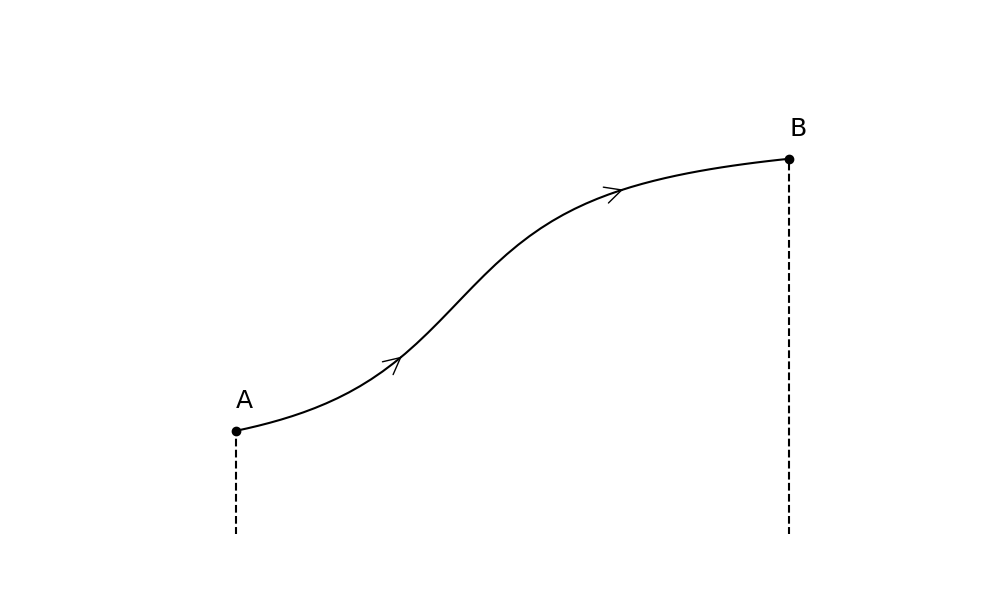
\includegraphics[width=\textwidth]{integraldelinea.png}
        }
      \end{wrapfigure}
      \noindent$C=\{M\in\bbR^2\colon\exists t\in\left[a,b\right],M\left(f\left(t\right),
      g\left(t\right)\right)\}$ con $f$, $g$ derivables en $\left[a,b\right]$, $A\left(f
      \left(a\right),g\left(a\right)\right)$ y $B\left(f\left(b\right),g\left(b\right)
      \right)$.\\ \\Consideremos $\ovl{V}\left(P\left(x,y\right),Q\left(x,y\right)
      \right)$ y sea $w$ la 1-forma diferencial, i.e. $w=P\left(x,y\right)dx + Q\left(x,y
      \right)dy$\\
    \subsection*{}
    \vspace{0.5cm}
    \definicion{Integral de línea}{
      $\gamma_{\ovl{AB}}=\int_{\ovl{AB}}\ovl{V}\left(M\right)\cdot\ovl{dM}=\int_{\ovl{AB}}
      \left(P\left(x,y\right)dx+Q\left(x,y\right)dy\right)=\int_{\ovl{AB}}w$ y tenemos
      $$\gamma_{\ovl{AB}} = \int_{\ovl{AB}}w = \int_{a}^{b}\left[P\left(f\left(t\right),g
      \left(t\right)\right)f'\left(t\right)+Q\left(f\left(t\right),g\left(t\right)g'\left(t
      \right)\right)\right]dt \rightarrow \text{¡Integral de Riemann!}$$ Donde $dx=f'
      \left(t\right)dt$,   $dy=g'\left(t\right)dt$
    }
    \ejemplo{Sea $w=\frac{y}{x^2+y^2}dx-\frac{x}{x^2+y^2}dy,\left(x,y\right)=\left(0,0
    \right)$, necesistamos una curva parametrizada.}{
      Sea\setlength\extrarowheight{0pt}
      $C = \begin{cases}\begin{aligned}
        x=\cos\theta\\
        y=\sin\theta
      \end{aligned}\end{cases} \text{con $\theta\in\left[0,2\pi\right]$}$, denotamos $C^+$ a la curva
      en el sentido trigonométrico.\\Nos piden calcular
      $\gamma_{C^+}=\int_{C^+}w$. \\Volvemos a la definición: $\int_{C^+}w=\int_{0}^{2\pi}
      \left[\sin\theta\left(-\sin\theta\right)-\cos\theta\left(\cos\theta\right)\right]
      d\theta=-\int_{0}^{2\pi d\theta}=-2\pi$ \par
      \vspace{0.2cm}Donde $P\left(f\left(\theta\right),g\left(\theta\right)\right) =
      \sin\theta$ y $Q\left(f\left(\theta\right),g\left(\theta\right)\right) =
      -\cos\theta$. Y también,$f'\left(\theta\right) = -\sin\theta$ y $g'\left(\theta
      \right) = \cos\theta$
    }
    \comentario{
      $\gamma_{\ovl{AB}}=\int_{\ovl{AB}}\ovl{V}\left(M\right)dM\left(t\right)=\int_{a}^{b}
      \ovl{V}\left(M\left(t\right)\right)\cdot\ovl{T}\left(t\right)\cdot dt$ \hspace{1cm}
      Donde $\ovl{V}\left(M\left(t\right)\right)$ puede ser un campo de fuerzas.
    }
    \ejemplo{Sea $w=xy\ dx+y^2\ dy+dz$ una 1-forma diferencial en $\bbR^3$ y sea $C$ la
    curva orientada en $\bbR^3$ con la parametrización $\ovl{V}\left(t\right)=\left(
    t^2,t^3,1\right)$ con $t \in \left[0,1\right]$. Calcular $\int_{C}w$}{
      $\int_{C}w=\int_{0}^{1}\left[t^5\left(2t\right)+t^6\left(3t^2\right)+0\right]dt=
      \frac{13}{21}$
    }
    \clearpage
    \teorema{}{
      Si $\ovl{V}$ es un \textbf{campo de gradiente} (i.e. $\ovl{V}=\ovl{\text{grad}}
      \varphi=\ovl{\nabla}\ovl{V}$), $\gamma_{\ovl{AB}} =\int_{\ovl{AB}}\ovl{V}\left(
      M\right)\cdot\ovl{dM}=\int_{\ovl{AB}}\ovl{\nabla}\varphi\left(M\right)\cdot
      \ovl{dM} = \int_{\ovl{AB}}d\varphi=\varphi\left(B\right)-\varphi\left(A\right)$
    }
    \comentario{
      \begin{itemize}
        \item La circulación de un campo de gradiente no depende del camino, solamente
              de los valores del campo escalar $\varphi$ definido por $\ovl{V}=\ovl{\nabla}
              \varphi$ en los extremos del camino $\ovl{AB}$.
        \item $\gamma_{\ovl{AB}}=0$ si $A$ y $B$ están en la misma curva de nivel de
              $\varphi$
      \end{itemize}
    }
    \teorema{}{
      \hspace{-0.9cm}
      \setlength{\tabcolsep}{17pt}
      \begin{tabular}{l l}
        $\int_{\ovl{AB}}\left(w_1+w_2\right)=\int_{\ovl{AB}}w_1+\int_{\ovl{AB}}w_2$&
        $\left(\ovl{V_1}\left(M\right)+\ovl{V_2}\left(M\right)\right)\ovl{dM}=
          \int_{\ovl{AB}}\ovl{V_1}\left(M\right)dM +\int_{\ovl{AB}}\ovl{V_2}\left(
          M\right)dM$\\
        $\forall\lambda\in\bbR\int_{\ovl{AB}}\lambda w_1=\lambda\int_{\ovl{AB}}w_1$&
        $\forall\lambda\in\bbR\int_{\ovl{AB}}\lambda\ovl{V_1}\left(M\right)dM=
          \lambda\int_{\ovl{AB}}\ovl{V_1}\left(M\right)dM$ \\
        Si $C\in\ovl{AB}$, entonces $\int_{\ovl{AB}}w=\int_{\ovl{AC}}w+
          \int_{\ovl{CB}}w$&
        $\int_{\ovl{AB}}\ovl{V_1}\left(M\right)dM=
          \int_{\ovl{AC}}\ovl{V_1}\left(M\right)dM+\int_{\ovl{CB}}\ovl{V_1}
          \left(M\right)dM$\\
        \multicolumn{2}{l}{$\int_{\ovl{AB}}w=-\int_{\ovl{BA}}w$ (Hay que cambiar la
          parametrización para mostrarlo)}
      \end{tabular}
    }
    \corolario{}{
      Si $\ovl{AB}$ es una curva cerrada, entonces $A=B$, y si $\ovl{V}$ es un campo
      de gradiente, entonces $\int_{\ovl{AB}}\ovl{V}\left(M\right)\ovl{dM}=0$
    }
    \definicion{Campo conservativo}{
      Se dice que un campo vectorial es conservativo si la circulación del campo
      vectorial es nula en toda curva cerrada.
    }
    \teorema{}{
      Sean $A$ y $B$ dos puntos del plano, la circulación de un campo conservativo no
      depende del camino para ir de $A$ a $B$.
    }
    \teorema{}{
      Si $\ovl{V}$ es un campo de gradiente, entonces $\ovl{V}$ es un campo conservativo.
    }
    \ejercicio{Sea $\ovl{V}\left(M\right)=\frac{3x^2+y^2}{y^2}\hat{x}-\frac{2x^3}{y^3}
    \hat{y}$\\\begin{itemize}
      \item Sean $A\left(-1,1\right)$ y $B\left(1,1\right)$ calcular $\gamma_{\ovl{AB}}$
            con $\ovl{AB}=\left[A\ B\right]$ (segmento).
      \item Idem con $\ovl{AB}\equiv$ semicírculo de centro $\Omega\left(0,1\right)$
    \end{itemize}
    }
    {
      Ver TD2
    }
    \teorema{}{
      Si $\ovl{V}$ es un campo conservativo, entonces $\ovl{V}$ es un campo de gradiente.
    }
    \comentario{
      Destacar que ahora tenemos la doble implicación entre campo conservativo y de gradiente.
    }
  \section{Longitud de una curva}
    \definicion{Longitud de una curva}{
      Sea $\gamma\colon\left[a,b\right]\longrightarrow\bbR^n$ una curva paramétrica de
      clase $\mcC_1$, la \textbf{longitud de $\gamma$} viene dada por la expresión:
      $$L\left(\gamma\right)=\int_{a}^{b}\norm{\gamma '\left(t\right)}dt$$
    }
    \comentario{
      Si $\gamma\left(t\right)\setlength\extrarowheight{0pt}\begin{pmatrix}x_1(t)\\
      \vdots\\x_n(t)\end{pmatrix}$ en coordenadas cartesianas, entonces
      $L\left(\gamma\right)=\int_{a}^{b}\sqrt{x_1'(t)^2+\hdots x_2'(t)^2}dt$
    }
    \ejercicio{Halla la longitud de arco de la siguiente curva: $\gamma\left(t\right)
    =\left(3t,3t^2,2t^3\right)$ entre los puntos $\left(0,0,0\right)$ y $\left(3,3,2
    \right)$}{
      $L\left(\gamma\right)=\int_{\left(0,0,0\right)}^{\left(3,3,2\right)}\sqrt{
      3^2+36t^2+36t^4}dt=\int_{0}^{1}\sqrt{9+36t^2+36t^4}dt=3\int_{0}^{1}\sqrt{
      4t^4+4t^2+1}dt=3\int_{0}^{1}\left(2t^2+1\right)dt=\left[2t^3+3t\right]^1_0=5$
    }
    \ejercicio{Halla la longitud de arco de la siguiente curva: $\gamma\left(t\right)
    =\setlength\extrarowheight{0pt}\begin{cases}\begin{aligned}\left(\cos(t),\sin(t),3t\right)\text{
    si $0\leq t\leq \pi$}\\\left(-1,-t+\pi,3t\right)\text{ \ \ si $\pi\leq t \leq 2\pi$}
    \end{aligned}\end{cases}$}{
      Tenemos $\gamma_1'\left(t\right)=\setlength\extrarowheight{0pt}\begin{pmatrix}
      -\sin t\\\cos t\\3\end{pmatrix}\ $ y $\ \gamma_2'\left(t\right)=
      \setlength\extrarowheight{0pt}\begin{pmatrix}0\\-1\\3\end{pmatrix}$,
      $\norm{\gamma_1\left(t\right)}=\sqrt{\sin^2t+\cos^2t+3^2}=\sqrt{10}\ $ y
      $\ \norm{\gamma_2\left(t\right)}=\sqrt{10}$, \\$L\left(\gamma_1\left(t\right)
      \right)=\int_{0}^{\pi}\sqrt[]{10}=\pi\ \sqrt[]{10}\hspace{1cm}
      L\left(\gamma_2\left(t\right)\right)=\pi\ \sqrt[]{10}\implies
      L\left(\gamma\left(t\right)\right)=L\left(\gamma_1\left(t\right)\right)+
      L\left(\gamma_2\left(t\right)\right)=\pi\ \sqrt[]{10}+\pi\ \sqrt[]{10}=
      2\pi\ \sqrt[]{10}$
    }
\chapter{Integrales dobles}
  \section{Introducción}
    \noindent Sea $\mcD=\left[a,b\right]\times\left[c,d\right]$ (con $a<b$ y $c<d$)
    un rectángulo. Como se hizo con la integral simple, vamos a subdividir
    los intervalos de los ejes (abcisas y ordenadas). Sean las particiones de
    $\left[a,b\right]$ y $\left[c,d\right]$\\ \setlength\extrarowheight{0pt}
    $\begin{cases}\begin{aligned}a=x_0<x_1<\hdots<x_n=b\\c=y_0<y_1<\hdots<y_m=d\end{aligned}\end{cases}$
    Obtenemos así las mallas, o Rectángulos Elementales:
    $R_{ij}=\left[x_{i-1},x_i\right]\times\left[y_{j-1},y_j\right]$

    \vspace{0.6cm}
    \hspace*{5.65cm}\textbf{\large 1. Subdivisión o malla regular}
    \vspace{-1.4cm}
    \begin{figure}[h]
      \begin{floatrow}
        \ffigbox{\hspace{-6.3cm}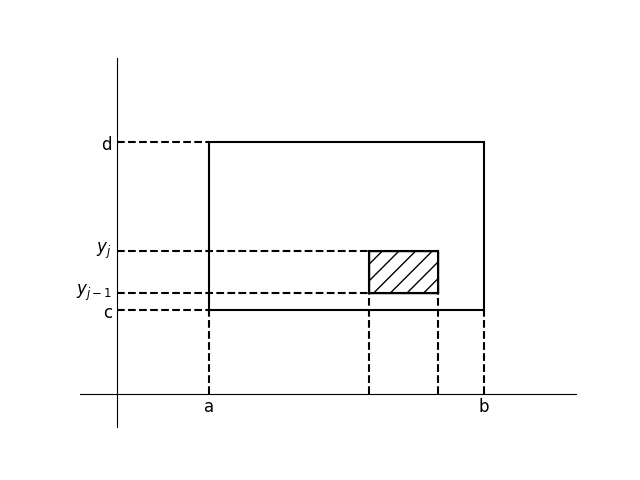
\includegraphics[width=.4\textwidth]{integralesdobles.png}}{}
        \capbtabbox{
          \hspace{-5cm}
          \begin{tabularx}{0.56\textwidth}{XXX}
            \vspace{-1.65cm}
            $\begin{cases}
              \begin{aligned}
                &x_i=x_{i-1}+h, &i=1,\text{...},n\\
                &y_j=x_{j-1}+k, &j=1,\text{...},m\\
              \end{aligned}
            \end{cases}$&\vspace{-1.4cm}\hspace*{1.7cm} con &
            \vspace{-1.65cm}
            $\begin{cases}
              \begin{aligned}
                &x_i=x_{i-1}+h, &i=1\text{,...,}n\\
                &y_j=x_{j-1}+k, &j=1\text{,...,}m\\
              \end{aligned}
            \end{cases}$\\
            \multicolumn{3}{l}{\vspace{0.13cm}\textbf{\large 2. Función escalonada en el rectángulo $\mcD$}}\\
            \multicolumn{3}{l}{
              \begin{tabular}[c]{@{}l@{}}Sean $\mcD = \left[a,b\right]\times\left[c,d\right]$ un rectángulo
                y $f\colon\mcD\rightarrow\bbR$ tal que:\\
                \hspace*{0.5cm}1. $f$ es acotada en $\mcD$\\
                \hspace*{0.5cm}2. $\forall x\in\left(x_{i-1},x_i\right)\times\left(y_{j-1},y_j\right), f(x)=\mcK_{ij}\in\bbR$\\
                Se dice que $f$ es escalonada.
              \end{tabular}
              }
          \end{tabularx}
        }{}
      \end{floatrow}
    \end{figure}

    \noindent\textbf{\large 3. Definición de la integral doble de una función}\\
    \vspace{0.13cm}\noindent Sean $\mcD=\left[a,b\right]\times\left[c,d\right]$ y $f$ una función escalonada a una malla regular de $\mcD$,
    se define la integral doble con: $\mcI\left(f\right)=\sum\limits_{i=1}^{n}\sum\limits_{j=1}^{m}\mcK_{ij}\left(x_i-x_{i-1}\right)
    \left(y_j-y_{j-1}\right)$ (la malla más fina posible)\\
    Se llama $\mcI\left(f\right)$ a la integral doble de $f$ sobre $\mcD$ denotada: $\mcI\left(f\right)=\iint_{\mcD}f\left(x,y\right)\ dxdy$\\

    \vspace{0.4cm}\noindent\textbf{\large 4. Criterio de integrabilidad de funicones }
    \definicion{Función integrable en $\mcD$}{
      Sea $f\colon\mcD\rightarrow\bbR$, se dice que $f$ es integrable en $\mcD$ si $\forall\epsilon >0,\exists f_1,f_2$ escalonadas en $\mcD$
      tales que: \begin{enumerate}
        \item $f_1\leq f\leq f_2$
        \item $\left|\iint_{\mcD}f_2\left(x,y\right)\ dxdy - \iint_{\mcD}f_1\left(x,y\right)\ dxdy\right|<\epsilon$
      \end{enumerate}
    }
    \comentario{
      El segundo punto es equivalente a cuando en una variable hablábamos de la diferencia de la suma superior y la suma inferior debe ser menor a épsilon
      $\left|\mcS_s-\mcS_i\right|<\epsilon$
    }

    \teorema{}{
      Sea $f\colon\mcD\rightarrow\bbR$ integrable en $\mcD$ y sea $\mcM_{ij}\in\left(x_{i-1},x_i\right)\times\left(y_{j-1},y_j\right)$ y sea
      $\delta_m,n=\sum\limits_{i=1}^{n}\sum\limits_{j=1}^{m} f\left(\mcM_{ij}\right)\left(x_i-x_{i-1}\right)\left(y_j-y_{k-1}\right)$,
      entonces $\lim\limits_{\left(m,n\right)\to\left(+\infty,+\infty\right)}\delta_{m,n} \in\bbR$ y denotamos $\lim\limits_{m,n}\delta_{m,n}
      =\iint_{\mcD}f\left(x,y\right)\ dxdy$ llamada integal doble de $f$ en $\mcM$.
    }
    \comentario{
      La condición del teorema anterior es que $f$ tiene que ser integrable, pero no tiene porqué ser escalonada.
    }
    \comentario{
      Al definir la malla regular, definimos $h=\frac{b-a}{n} y k=\frac{d-c}{m}$, que tenderán a cero cuando $n$ y $m$ tiendan a infinito.
    }
    \teorema{}{
      Sea $f\colon\mcD\rightarrow\bbR$ definida y continua en $\mcD=\left[a,b\right]\times\left[c,d\right]$ entonces $f$ es integrable en $\mcD$,
      siempre que $mcD$ sea un compacto.
    }
    \comentario{
      Es interesante conocer el \textit{Teorema de Pikoliv}, que nos dice que el producto cartesiano de compactos es un compacto.
    }
    \teorema{}{
      Sean $f$ y $g$ dos funciones integrables en $\mcD$, entonces:
      \begin{enumerate}
        \item $\iint_\mcD\left(f+g\right)\left(x,y\right)\ dxdy = \iint_\mcD\left(f(x,y)+g(x,y)\right)\ dxdy =
              \iint_\mcD f(x,y)\ dxdy + \iint_\mcD g(x,y)\ dxdy$\\

              \vspace{-0.3cm}"La integral doble de la suma es la suma de integrales"

        \item $\forall\lambda\in\bbR ,\iint_\mcD\lambda f(x,y)\ dxdy = \lambda\iint_\mcD f(x,y)\ dxdy$
        \item $\forall (x,y)\in\mcD ,f(x,y)\leq g(x,y)\implies\iint_\mcD f\ dxdy\leq\iint_\mcD g\ dxdy$
        \item $\abs{f}$ integrable en $\mcD \implies \left|\iint_\mcD f(x,y)\ dxdy\right|\leq\iint_\mcD\left|f(x,y)\right|\ dxdy$
      \end{enumerate}
    }
    \comentario{
      \begin{wrapfigure}{l}{.17\textwidth}
        \vspace{-0.5cm}
        \vspace{-1\intextsep}
        \ffigbox[\textwidth]{}{
          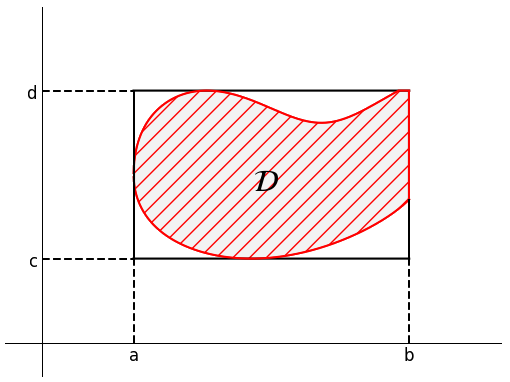
\includegraphics[width=\textwidth]{comentario4.1.3.png}
        }
      \end{wrapfigure}
      \vspace{0.3cm}Si $\mcD \subset \bbR^2$ es un dominio 'regular', definimos
      $\mcD$ rectángulo con $\tilde{f}$ en $\mcD'$ tal que:

      \vspace{0.3cm}$\tilde{f}=
      \begin{cases}
        \centering
        \begin{aligned}
          &f \text{ en }\mcD\\
          &f \text{ en }\mcD'\setminus\mcD\\
        \end{aligned}
      \end{cases}$ entonces $\ \ \ \ \boxed{\iint_{\mcD'}\tilde{f}\ dxdy = \iint_\mcD f\ dxdy}$

    }
    \comentario{
      Cuando $f$ es una función positiva sobre una región rectangular $\mcR$ del plano, podemos interpretar la integral doble
      de $f$ sobre $\mcR$ como el volumen de la región tridimensional sobre el plano acotada abajo por $\mcR$ y arriba por la
      superficie $z=f(x,y)$
    }
    \clearpage
  \section{Teoremas de Fubini}
    \teorema{Fubini en un rectángulo (versión débil)}{
      Sea $R$ un rectángula de $\bbR^2$, $R=\left[a,b\right]\times\left[c,d\right]$
      y sea $f$ una función integrable sobre $R$, tenemos: $$ \iint_{R}f\left(
      x,y\right)dxdy=\int_{a}^{b}\left(\int_{c}^{d}f\left(x,y\right)dy\right)dx=
      \int_{c}^{d}\left(\int_{a}^{b}f\left(x,y\right)dx\right)dy$$ (las integrales
      dobles son permutables)
    }
    \ejemplo{Calcular $I=\iint_A e^{x+y}dxdy$ con $A=\left[0,1\right]\times\left[0,2
    \right]$}{
      $I=\iint_A e^xe^ydxdy=\int_{0}^{1}e^xdx\cdot\int_{0}^{2}e^ydy=\left[e^x
      \right]^1_0\cdot\left[e^y\right]_0^2=\left(e-1\right)\left(e^2-1\right)$
    }
    \ejemplo{Calcular $I=\iint_R f\left(x,y\right)dxdy$ con $R=\left[0,2\right]
    \times\left[0,2\right]$ y $f$ definida en $R$ por $f\left(x,y\right)=16-x^2-2y^2$}{
        $I=\iint_R f\left(x,y\right)dxdy=\int_{0}^{2}\int_{0}^{2}16-x^2+2y^2dxdy=
        \int_{0}^{2}\left[16x-\frac{1}{3}x^3-2y^2x\right]_0^2dy=
        \int_{0}^{2}32-\frac{8}{3}-4y^2dy=\left[32y-\frac{8}{3}y-\frac{4}{3}y^3
        \right]_0^2=64-\frac{16}{3}-\frac{32}{3}=48$
    }
    \teorema{Fubini versión fuerte}{
      \begin{itemize}
        \item Sean $\varphi_1$ y $\varphi_2$ dos funiciones continuas en un rectángulo
              compacto de $\left[a,b\right]$ de $\bbR$ (uniformemente continuas) tales
              que:\\$\forall x\in\left[a,b\right],\varphi_1\left(x\right)\leq\varphi_2
              \left(x\right)$ y sea $\mcD\subset\bbR^2$ tal que $\mcD=\left\{\left(
              x,y\right)\in\bbR^2\colon a\leq x\leq b, \varphi_1\left(x\right)\leq y
              \leq\varphi_2\left(x\right)\right\}$ Si $f\colon\mcD\longrightarrow\bbR$
              es continua en $\mcD$ (entonces $f$ es integrable en $\mcD$) tenemos:
              $$\iint_Df\left(x,y\right)dxdy=\int_{a}^{b}\left(\int_{\varphi_1\left(
              x\right)}^{\varphi_2\left(x\right)}f\left(x,y\right)dy\right)dx$$
        \item Sean $\psi_1$ y $\psi_2$ dos funciones continuas en un rectángulo
              compacto de $\left[c,d\right]$ de $\bbR$ tales que:\\
              $\forall x\in\left[c,d\right],\psi_1\left(y\right)\leq\psi_2
              \left(y\right)$ y sea $\mcD'\subset\bbR^2$ tal que $\mcD'=\left\{\left(
              x,y\right)\in\bbR^2\colon c\leq y\leq d, \psi_1\left(y\right)\leq x
              \leq\psi_2\left(y\right)\right\}$ Si $f\colon\mcD'\longrightarrow\bbR$
              es continua en $\mcD'$ tenemos:
              $$\iint_{D'}f\left(x,y\right)dxdy=\int_{c}^{d}\left(\int_{\psi_1\left(
              y\right)}^{\psi_2\left(y\right)}f\left(x,y\right)dx\right)dy$$ (la
              integral se hace de forma horizontal).
      \end{itemize}
    }
    \ejemplo{Calcular $\iint_\mcD f\left(x,y\right)dxdy$ con $\mcD=\left\{\left(x,y
    \right)\in\bbR^2\colon 0\leq x \leq1, x^2\leq y\leq x\right\}$ (no es un rectángulo),
    sobre la función $f\left(x,y\right)=x+y$}{
      \begin{wrapfigure}{r}{.26\textwidth}
        \vspace{-1.5cm}
        \ffigbox[\textwidth]{}{
          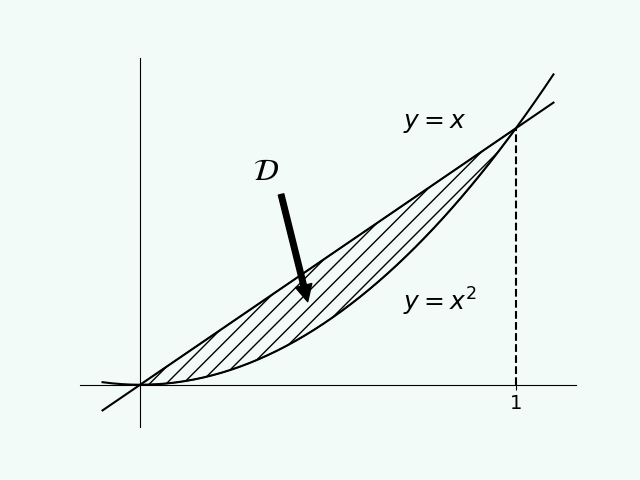
\includegraphics[width=\textwidth]{ejemplo4.1.3.png}
        }
      \end{wrapfigure}
      \vspace{0.6cm}
      $\iint_\mcD f\left(x,y\right)dxdy = \int_{0}^{1}\int_{x^2}^{x}f\left(x,y\right)
      dydx=\int_{0}^{1}\left[xy+\frac{y^2}{2}\right]^x_{x^2}dx=\vspace{0.2cm}\\
      \int_{0}^{1}\left(x^2+\frac{x^2}{2}-x^3-\frac{x^4}{2}\right)dx=\frac{3}{20}$
      \vspace{0.6cm}
    }
    \ejemplo{Calcular $\iint_\mcD e^xdxdy$ con $\mcD=\left\{\left(x,y\right)\in\bbR^2
    \colon 0\leq x\leq \log\left(y\right), 1\leq y\leq 2\right\}$}{
      \begin{wrapfigure}{r}{.26\textwidth}
        \vspace{-0.3cm}
        \vspace{-1\intextsep}
        \ffigbox[\textwidth]{}{
          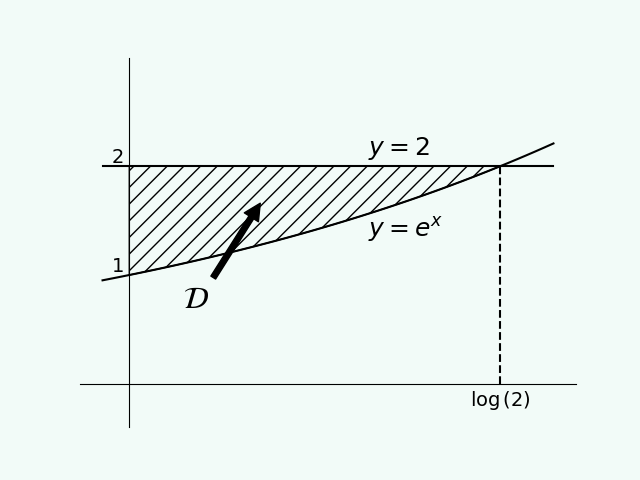
\includegraphics[width=\textwidth]{ejemplo4.1.4.png}
        }
      \end{wrapfigure}
      \vspace{0.6cm}
      Como $f\left(x,y\right)\in\mcC_0\left(\bbR^2\right)\Rightarrow\text{Podemos
      aplicar el \textit{Teorema de Fubini}}$\vspace*{0.2cm}\\\setlength\extrarowheight{0pt}
      $\begin{cases}\begin{aligned}
        &\iint_{\mcD}e^xdxdy=\int_1^2\int_0^{\log y}e^xdxdy=\int_{1}^{2}
          \left(y-1\right)dy=\left[\frac{y^2}{2}-y\right]_1^2=\frac{1}{2}\\
        &\iint_{\mcD}e^xdxdy=\int_0^{\log y}\int_1^2e^xdydx=\int_{0}^{\log 2}
        e^xdydx=\int_0^{\log 2}e^x\left(2-e^x\right)dx=\frac{1}{2}
      \end{aligned}\end{cases}$
      \vspace{0.2cm}
    }
  \section{Teorema de cambio de variable}
    \noindent Vamos a preparar la base para un teorema considerando un paralelogramo $\mcA_{(CA\ CB)}=\norm{\vec{OA}\wedge\vec{OB}}$
    Sea $T\colon\bbR^2\longrightarrow\bbR^2$ lineal (rotación, homotecia, ...) $\mcA\left(T\left([0,1]^2\right)\right)=\norm{T\left(\vec{e_1}\right)\wedge\left(\vec{e_2}\right)}$
    
    \begin{center}
      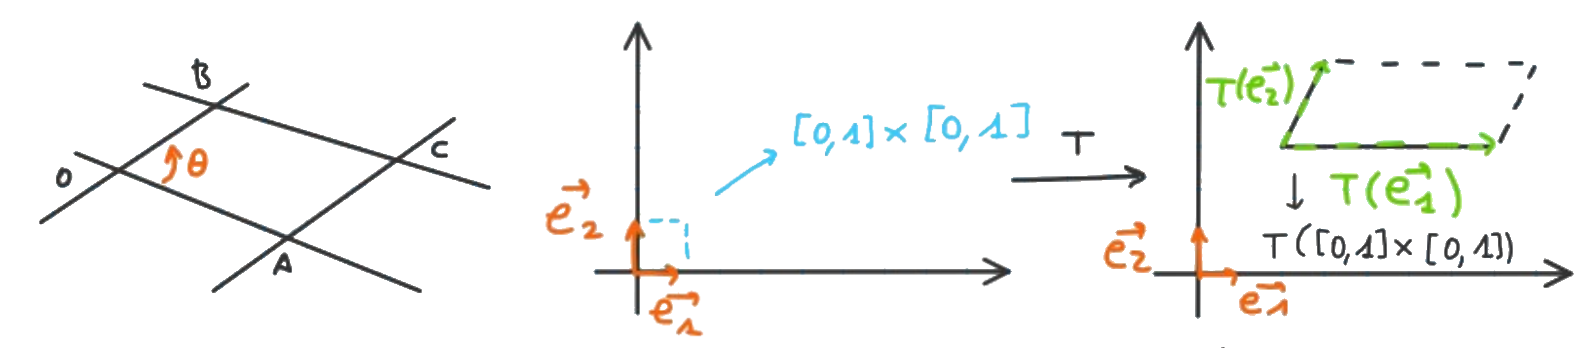
\includegraphics[width=\textwidth]{cambioVar.png}
    \end{center}

    \noindent Tenemos $T\left(\vec{e}_1\right)=T_{11}\vec{e}_1+T_{21}\vec{e}_2$ (porque tomamos como base $\vec{e}_1,\vec{e}_2$, $T_{ij}$ serán únicos). \textit{idem} con $\vec{e}_2\colon$
    $\begin{cases}
      \begin{aligned}
        &T\left(\vec{e}_1\right) = T_{11}\vec{e}_1+T_{21}\vec{e}_2 \\
        &T\left(\vec{e}_2\right) = T_{12}\vec{e}_1+T_{22}\vec{e}_2 \\
      \end{aligned}      
    \end{cases}$ lo que nos da $\norm{T\left(\vec{e}_1\wedge\vec{e}_2\right)}=\abs{\text{det}(T)}=
    \begin{vmatrix}
      T_{11} & T_{12} \\
      T_{21} & T_{22} \\
    \end{vmatrix}$ que nos habla de la matriz asociada a la aplicación lineal $T$.

    \noindent Entonces, $\mcA\left(T\left([0,1]^2\right)\right)=\abs{\text{det}(T)}$.\\

    \noindent De forma general, sean $i=1,2$ $L_i>0$: $\mcA\left(T\left([0,L_1]\right)\times T\left([0,L_2]\right)\right)=
    \norm{T\left(L_1\vec{e}_1\right)\wedge T\left(L_2\vec{e}_2\right)}=L_1L_2\abs{\text{det}(T)}$. 
    
    \noindent $L_1\vec{e}_1$ es un vector colineal a $L_1$. Si hacemos un cambio de variable, cambia la geometría y con ello el área.

    \vspace{0.4cm}\noindent Sea 
    $\begin{aligned}
      \phi\colon &\Omega\subset\bbR^2\hspace{0.2cm}\longrightarrow\mcD\in\bbR^2\\
      &U(u_1,u_2)\longmapsto\phi(U)=\left(\phi_1(U),\phi_2(U)\right)\\
    \end{aligned}$ y sea $(x_1,x_2)\in\bbR^2$ denotamos $\phi(U)=M(x_1,x_2)=\left(\phi_1(u_1,u_2),\phi_2(u_1,u_2)\right)$
    
    \vspace{0.4cm}\noindent $\implies \phi\left(\Omega\right)=\mcD$, Como vemos en la siguiente figura, $\phi$ deforma el rectángulo inicial en otra cosa.
    
    \begin{center}
      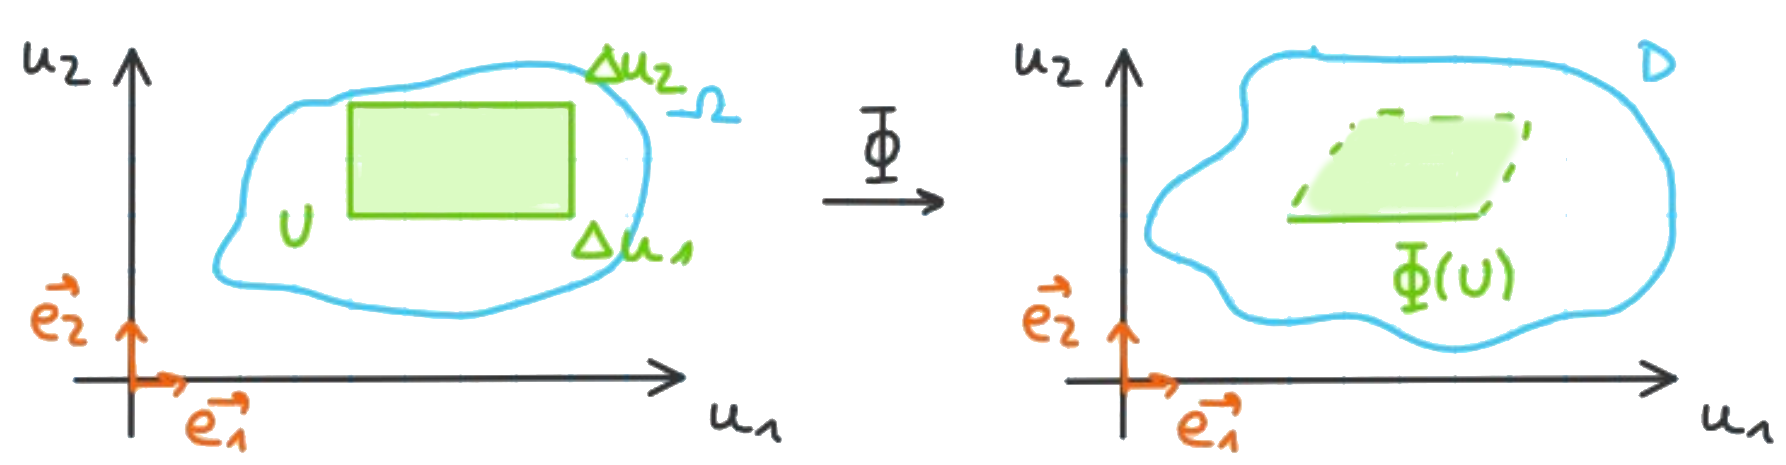
\includegraphics[width=\textwidth]{cambioVar2.png}
    \end{center}

    \clearpage
    \noindent Suponemos que:
    \begin{enumerate}
      \item $\phi$ es una biyección
      \item $\phi$ y $\phi^{-1}$ son de clase $\mcC_1$ en su dominio respectivo.
    \end{enumerate}
    Es decir, que $\phi$ sea un $\mcC_1$-difeomorfismo. 
    
    \noindent Tenemos entonces $\phi\left(U+h\right)=\phi(U)+D_{\phi}(U)\cdot h +o(h)$
    \hspace{1cm}con $D_{\phi}(U)=
    \begin{vmatrix}
      \frac{\partial\phi_1(U)}{\partial u_1}& \frac{\partial\phi_1(U)}{\partial u_2} \\
      \frac{\partial\phi_2(U)}{\partial u_1}& \frac{\partial\phi_2(U)}{\partial u_2} \\
    \end{vmatrix}$ 

    \noindent Si $\Delta u_1$ y $\Delta u_2$ son 'pequeños' entonces $\mcA\left(\phi\left([u_1,u_1+\Delta u_1]\times[u_2,u_2+\Delta u_2]\right)\right)$ es el área 
    de un paralelogramo, es decir $\norm{D_{\phi}(U)\left(\Delta u_1\vec{e}_1\right)\wedge D_\phi\left(\Delta u_2\vec{e}_2\right)}$, donde $D_\phi(U)$ es la imagen de la parte lineal de $\phi$.

    \vspace{0.2cm}\noindent Tenemos finalmente, 
    $$\hspace{-16pt}\mcA\left(\phi\left([u_1,u_1+\Delta u_1]\times[u_2,u_2+\Delta u_2]\right)\right)=\Delta u_1\Delta u_2\norm{D_{\phi(U)}\left(\vec{e}_1\right)\wedge D_{\phi(U)}\left(\vec{e}_2\right)}=
    \Delta u_1\Delta u_2\abs{\text{det}\left(D_\phi\left(u_1,u_2\right)\right)} \leftarrow\text{ ¡El Jacobiano!}$$

    \teorema{Cambio de variable}{
      Sea $f\in\mcC_0(\ovl{\mcD})$ (donde $\mcD$ es un abierto acotado de $\bbR^2$) entonces para todo $\phi$ $\mcC_1$-difeomorfismo de $\ovl{\Omega}$ en $\ovl{\mcD}$ tenemos:
      $$\iint_\mcD f(x_1,x_2)\ dx_1dx_2=\iint_\Omega f\left(\phi(u_1,u_2)\right)\abs{\text{det}\left(\mcD_\phi(u1,u2)\right)}\ du_1du_2$$
    }
    \comentario{
      \textbf{Aplicación: Cambio a polares}
      $\begin{cases}
        \begin{aligned}
          &x=r\cos\theta\\
          &y=r\sin\theta\\
        \end{aligned}
      \end{cases}\implies g\left(r,\theta\right)=\left(r\cos\theta,r\sin\theta\right)$\\

      $\abs{J\left(r,\theta\right)}=
      \begin{vmatrix}
        \frac{\partial x}{\partial r}& \frac{\partial x}{\partial \theta}\\
        \frac{\partial y}{\partial r}& \frac{\partial y}{\partial \theta}\\
      \end{vmatrix}=
      \begin{vmatrix}
        \cos\theta& -r\sin\theta\\
        \sin\theta&  r\cos\theta\\
      \end{vmatrix}$\\
      
      Entonces:
      $$\iint_\mcD f(x,y)\ dxdy=\iint_\Omega f\left(r\cos\theta,r\sin\theta\right)r\ drd\theta$$
    }
    \ejemplo{Calcular $\iint_\mcD \frac{1}{1+x^2+y^2}\ dxdy$ con $\mcD=\left\{(x,y)\in\bbR^2:0\leq y\leq 1,0<x^2+y^2\leq 1\right\}$}{
      Usamos el cambio de variable de polares 
      $\begin{cases}
        \begin{aligned}
          &x = r\cos\theta\\
          &y = r\cos\theta\\
        \end{aligned}
      \end{cases} (x,y)\in\mcD \Leftrightarrow \begin{cases}
        \begin{aligned}
          &r\in[0,1]\\
          &\theta\in\left[0,\frac{\pi}{2}\right]
        \end{aligned}
      \end{cases}$

      Tenemos $1+x^2+y^2=1+r^2$

      $\iint_\mcD f(x,y)\ dxdy=\int_{0}^{1}\int_{0}^{\frac{\pi}{2}}\frac{1}{1+r^2}r\ d\theta dr=\frac{\pi}{2}\int_{0}^{1}\frac12\frac{2r}{1+r^2}\ dr=
      \frac{\pi}{4}\left[\log(1+r^2)\right]_0^1=\frac{\pi\log(2)}{4}$
    }

\section{Teorema de Green-Riemann}
    \noindent Si $f\in\mcC_1\left([a,b]\right)$ entonces $f(b)-f(a)=\int_a^b f'(t)\ dt$. Nos gustaría
    generalizar este resultado al plano.\\
    
    \begin{wrapfigure}[7]{l}{.23\textwidth}
      \vspace{-1\intextsep}
      \ffigbox[\textwidth]{}{
        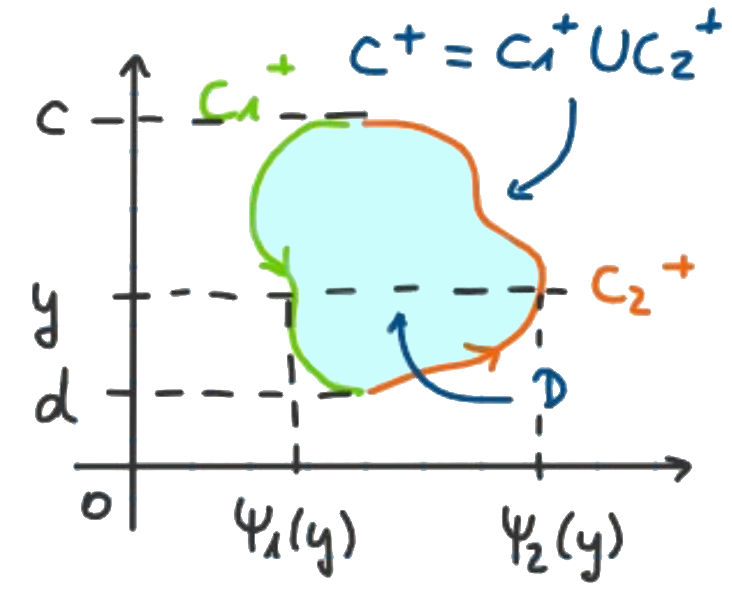
\includegraphics[width=\textwidth]{green0.png}
      }
    \end{wrapfigure}

    \noindent Sea $f$ una función que admita derivadas parciales continuas en $\overline{\mcD}\in\bbR^2\colon$

    \noindent$\iint_\mcD\ dxdy = \int_{y=c}^{y=d}\left(\int_{x=\psi_1(y)}^{x=\psi_2(y)}\frac{\partial f}{\partial x}(x,y)\ dx\right)\ dy=$
    $\int_{y=c}^{y=d}\left[f\left(\psi_2(y),y\right)-f\left(\psi_2(y),y\right)\right]\ dy$\\

    \noindent$C_2^+ = \left\{(x,y)\in\bbR^2,M_2(t)=\left(\psi_2(t),t\right)\right\}$ con $t\in[c,d]$\\
    $C_1^+ = \left\{(x,y)\in\bbR^2,M_1(t)=\left(\psi_2(t'),t'\right)\right\}$ con $t'\in[d,c]$\\
    
    \noindent Y aplicamos un cambio de variable para pasar de $[d,c]$ a $[c,d]$ en $C_2\colon$\\

    \noindent Sea $t=\alpha t' + \beta$ con $t\in[c,d]\colon$\hspace{0.6cm}
    $\begin{cases}\begin{aligned}
      &c=\alpha d + \beta\\
      &d=\alpha c + \beta\\
    \end{aligned}\end{cases}\implies c-d=\alpha(d-c)\implies\alpha = -1$\\

    \noindent Entonces, $\beta=c-\alpha d = c+d$. Tenemos, $t=-t'+c+d \Leftrightarrow t'=c+d-t$. Y con este resultado tenemos:\\
    $C_1^+=\left\{(x,y)\in\bbR^2,M_1(t)=\left(\psi_1(c+d-t),c+d-t\right)\right\}$ con $t\in[c,d]$\\

    \noindent Para estudiar la integral, debemos centrar nuestra atención en $\int_c^d f\left(\psi_2(t),t\right)\ dt$\\
    $\int_{C_2^+}f\ dy=\int_{C_2^+}0\ dx+ f\ dy=\int_c^d\vec{V}\left(M_2(t)\right)\cdot M_2'(t)\ dt$
    \hspace{0.3cm}con 
    $\vec{V}\begin{pmatrix} 0          \\ f \end{pmatrix} \;$,
    $M_2(t) \begin{pmatrix} \psi_2(t)  \\ t \end{pmatrix} \;$,
    $M_2'(t)\begin{pmatrix} \psi_2'(t) \\ 1 \end{pmatrix} \;$\\

    \noindent Entonces, $\int_{C_2^+}f\ dy=\int_{c}^{d}f\left(M_2(t)\right)\cdot 1\ dt=\int_{c}^{d}f\left(\psi_2(t),t\right)\ dt$\\
    
    \noindent $\int_{C^+}f\ dy=\int_{c}^{d}\vec{V}\left(M_1(t)\right)\cdot M_1'(t)\ dt$
    $=-\int_{c}^{d}f\left(M_1(t)\right)\ dt=-\int_{c}^{d}f\left(\psi_1(c+d-t),c+d-t\right)\ dt$
    $=\int_{d}^{c}f\left(\psi_1(s),s\right)\ ds=$\\
    $=-\int_{c}^{d}f\left(\psi_1(s),s\right)\ ds=\int_{C_1^+}f\ dy$
    
    \noindent \vspace{0.3cm}con
    $\vec{V}\begin{pmatrix} 0             \\ f     \end{pmatrix} \;$,
    $M_1(t) \begin{pmatrix} \psi_1 (c+d-t)\\ c+d-t \end{pmatrix} \;$,
    $M_1'(t)\begin{pmatrix} \psi_1'(c+d-t)\\ -1    \end{pmatrix} \;$
    \hspace{0.4cm}y\hspace{0.4cm}
    $\begin{cases}
      \begin{aligned}
        &s=c+d-t\\
        &ds=-dt
      \end{aligned}
    \end{cases}$

    En conclusión,
    $$\iint_\mcD\frac{\partial f}{\partial x}(x,y)\ dxdy=\int_{c}^{d}f\left(\psi_2(y),y\right)\ dy-\int_{c}^{d}f\left(\psi_1(y),y\right)\ dy=
    \int_{C_2^+}f\ dy+\int_{C_1^+}f\ dy=\int_{C^+}f\ dy$$

    \noindent Si repetimos con la derivada parcial respecto a $y$, de la misma manera obtenemos el mismo resultado, pero 
    cambiando el signo a causa de la orientación de la curva.
    
    \begin{empheq}[box=\fbox]{align}
      \iint_\mcD\frac{\partial f}{\partial x}(x,y)\ dxdy&=\ \ \ \int_{C^+}f\ dy\nonumber\\
      \iint_\mcD\frac{\partial f}{\partial y}(x,y)\ dydx&=     -\int_{C^+}f\ dy\nonumber
    \end{empheq}

    \teorema{Green-Riemann}{
      Sean $f,g\in\mcC_1\left(\overline{\mcD}\right)$ y sea $C^+$ la frontera orientada de $\mcD$, entonces:
      $$\iint_\mcD\left(\frac{\partial g}{\partial x}-\frac{\partial f}{\partial y}\right)\ dxdy = \int_{C^+}f\ dx+g\ dy$$
    }
    \comentario{
      \textbf{Aplicación del teorema de Green-Riemann}
      \begin{enumerate}
        \item Si $w=f\ dx+g\ dy$, entonces $dw=\left(\frac{\partial g}{\partial x}-\frac{\partial f}{\partial y}\right)\ dx\wedge dy$\\
              En el caso del cálculo integral, denotamos $dx\wedge dy\equiv dxdy$, lo que nos permie escribir $\iint_\mcD dw=\int_{\sigma(\mcD)}w$
        \item Si $\vec{V}\left(V_1,V_2\right)$, entonces $\iint_\mcD\left(\frac{\partial V_2}{\partial x}-\frac{\partial V_1}{\partial y}\right)\ dxdy=$
              $\int_{\sigma(\mcD)}V_1\ dx + V_2\ dy=\int_{\sigma(\mcD)\vec{V}(M)\cdot d\vec{M}}$\\
              Si $\frac{\partial V_2}{\partial x}-\frac{\partial V_1}{\partial y}=0$ en $\mcD$, entonces $w=V_1\ dx+V_2\ dy$ es cerrada, y si $\mcD$
              es un abierto estrellado de $\bbR^2$, entonces $w$ es exacta $\implies \vec{V}$ es un campo de gradiente.\\
              Entonces si $\frac{\partial V_2}{\partial x}-\frac{\partial V_1}{\partial y}=0$ en $\mcD\implies$
              $\int_\mcD\vec{V}(M)\cdot d\vec{M}=0\ \forall$curva cerrada.
      \end{enumerate}
    }
    \comentario{
      Sea $f$ una función que admite derivadas parciales continuas ($\in\mcC_1$) y además satisface la \textit{Ecuación de Laplace}
      $\left(\frac{\partial^2f}{\partial x^2}+\frac{\partial^2f}{\partial y^2}=0\right)$, entonces $\int_C\frac{\partial f}{\partial y}\ dx-\frac{\partial f}{\partial x}\ dy=0$\\

      Si aplicamos el \textit{Teorema de Green-Riemann}:
      $$\int_C\frac{\partial f}{\partial y}\ dx-\frac{\partial f}{\partial x}\ dy=\iint_\mcD\left[\frac{-\partial^2f}{\partial x^2}-\frac{\partial^2f}{\partial y^2}\right]\ dxdy=0$$
    }
    \comentario{
      El \textit{Teorema de Green-Riemann} se cumple también para una región con un número finito de agujeros,
      siempre que las curvas sean simples, cerradas y regulares. Debemos integrar sobre cada componente 
      de la frontera en la dirección en la que la región $R$ se mantiene a la izquierda mientras avanzamos.
      ¿Qué significa esto? Es una forma de elegir el sentido en la frontera.\\ 

      En la figura de la izquierda, hay que dejar la zona azul a nuestra izquierda (valga la redundancia). 
      \centering
      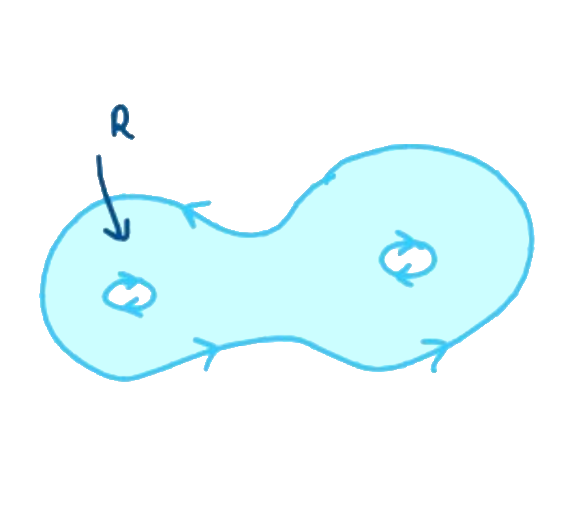
\includegraphics[width=.25\textwidth]{comentarioGR1.png}
      \hspace{2cm}
      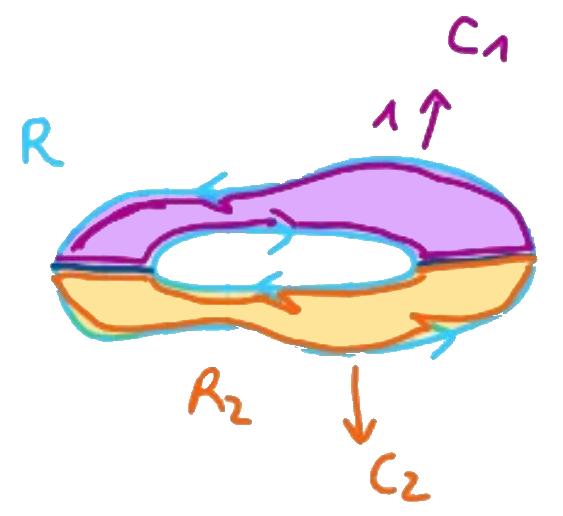
\includegraphics[width=.25\textwidth]{comentarioGR2.png}
      
      \begin{flushleft} 
      En la práctica, se crean dos regiones (arriba y abajo). Así, nos quitamos el hueco y tenemos dos curvas 
      que cumplen las condiciones.\\
      \vspace{0.4cm}
      $\iint_R\left(\frac{\partial Q}{\partial x}-\frac{\partial P}{\partial y}\right)\ dxdy = \iint_{R_1}\left(\frac{\partial Q}{\partial x}-\frac{\partial P}{\partial y}\right)\ dxdy
      +\iint_{R_2}\left(\frac{\partial Q}{\partial x}-\frac{\partial P}{\partial y}\right)\ dxdy = \int_{C_1}P\ dx+Q\ dy+\int_{C_2}P\ dx+Q\ dy=$\\
      $\int_C P\ dx+Q\ dy$
      \end{flushleft}
    }

    \subsection{Cálculo de Área}
      \subsubsection*{Caso particular}
        \noindent Supongamos que $\frac{\partial V_2}{\partial x}-\frac{\partial V_1}{\partial y}=1$ en $\mcD$
        $$\mcA\left(\mcD\right)=\iint_{\sigma\mcD}1\ dxdy=\int_{\sigma\mcD}V_1\ dx+V_2\ dy \hspace{1cm} \text{ y podemos elegir }\ \ 
        \vec{V}\begin{pmatrix} 0 \\ x \end{pmatrix} \text{ ó }\vec{V}\begin{pmatrix} -y \\ 0 \end{pmatrix} \text{ ó }
        \vec{V}\frac12\begin{pmatrix} -y \\ x \end{pmatrix}\implies$$
        $$\implies \mcA\left(\mcD\right)=\int_{\sigma\mcD}x\ dy=
        \int_{\sigma\mcD}y\ dx=\frac12\int_{\sigma\mcD}-y\ dx+x\ dy$$
        \ejemplo{Cálculo del área de una elpise $\mcD$}{
          Tomando la parametrización $\begin{cases}\begin{aligned}
              &x(t)=a\cos(t)\\
              &y(t)=b\sin(t)\\
          \end{aligned}\end{cases}$ con $t\in\left[0,2\pi\right]$
          $$\mcA\left(\mcD\right)=\frac12\int_{\sigma\mcD}-y\ dx+x\ dy=\int_{\sigma\mcD}\vec{V}\left(M\right)\ d\vec{M}=
          \int_{0}^{2\pi}\vec{V}\left(M(t)\right)\vec{M'}(t)\ dt$$
          y tenemos, $\vec{V}\frac12\begin{pmatrix} y \\ x \end{pmatrix}\implies \vec{V}\left(M(t)\right)=\frac12\left(-b\sin(t),a\cos(t)\right)$
          y $M'(t)=\left(-a\sin(t),b\cos(t)\right)$\\
          $\vec{V}\left(M(t)\right)\cdot\vec{M'}(t)=\frac12\left(ab\sin^2(t)+ab\cos^2(t)\right)=\frac12 ab$\hspace{1cm} 
          Finalmente, $\mcA\left(\mcD\right)=\int_{0}^{2\pi}\frac12 ab\ dt=\pi ab$
        }

      \subsubsection*{Flujo y divergencia de un campo vectorial}
      \vspace{0.2cm}
        \begin{wrapfigure}[1]{l}{.2\textwidth}
          \vspace{-1.6cm}
          \centering
          \ffigbox[\textwidth]{}{
            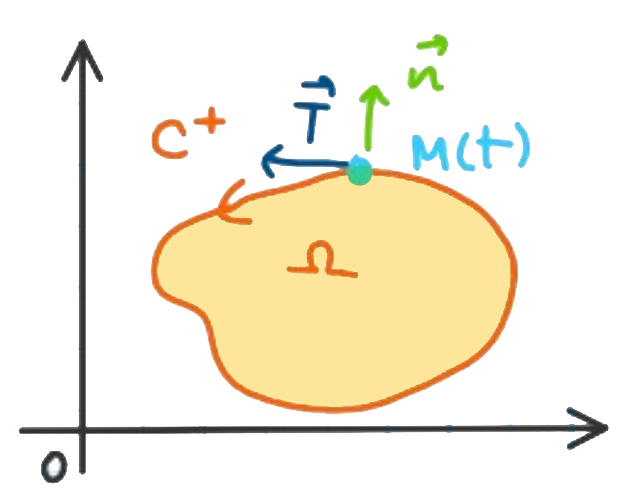
\includegraphics[width=\textwidth]{flujoYdiv.png}
          }
        \end{wrapfigure}

        \vspace{0.6cm}
        \noindent Tenemos $M(t)\left(f(t),g(t)\right)$\hspace{1cm}$\vec{T}(t)=\begin{pmatrix} f'(t) \\ g'(t) \end{pmatrix}$
        $\vec{n}=\begin{pmatrix} 0 & 1\\ -1 & 0 \end{pmatrix}\begin{pmatrix} f'(t) \\ g'(t) \end{pmatrix}=
        \begin{pmatrix} g'(t) \\ -f'(t) \end{pmatrix}$
        \vspace{1cm}
        
        \definicion{Flujo}{
          Sea $\vec{V}$ un campo vectorial, llamamos flujo de $\vec{V}$, denotado $\phi$ a través de 
          $\sigma\Omega$ a la cantidad
          $$\phi=\int_{\sigma\Omega}\vec{V}\cdot\ d\vec{n}=\iint_a^b\vec{V}\left(M(t)\right)\cdot\vec{n}\left(M(t)\right)\ dt$$
        }
        \teorema{Green-Ostrogradsky o \textbf{Teorema de la divergencia} (en $\bbR^2$)}{
          $$\phi=\int_{\sigma\Omega}\vec{V}\ d\vec{n}=\int_{a}^{b}\vec{V}\left(M(t)\right)\cdot\vec{n}\left(M(t)\right)\ dt=\iint_\Omega\nabla\cdot\vec{V}\ dxdy$$
        }
              
  \section{Superficies parametrizadas}
    \subsection{Introducción}
      \definicion{Superficie parametrizada}{
        Una \textbf{superficie parametrizada} es una función $\varphi\colon\mcD\subset\bbR^2\rightarrow\bbR^3$. La superficie denotada $S$ corresponde a 
        $\varphi(x,y)\forall(x,y)\subset\mcD$ es una imagen $S=\varphi\left(\mcD\right)$ 
      }

      \comentario{
        Podemos ver $\varphi(u,v)=\left(x(u,v),y(u,v),z(u,v)\right)$, y si además pedimos a $\varphi$ ser de clase $\mcC_1$ o diferenciable,
        entonces $S$ se denomina \textbf{Superficie diferienciable o de clase $\mcC_1$}.\\
        
        \begin{wrapfigure}[2]{l}{.35\textwidth}
          \vspace{-1\intextsep}
          \centering
          \ffigbox[\textwidth]{}{
            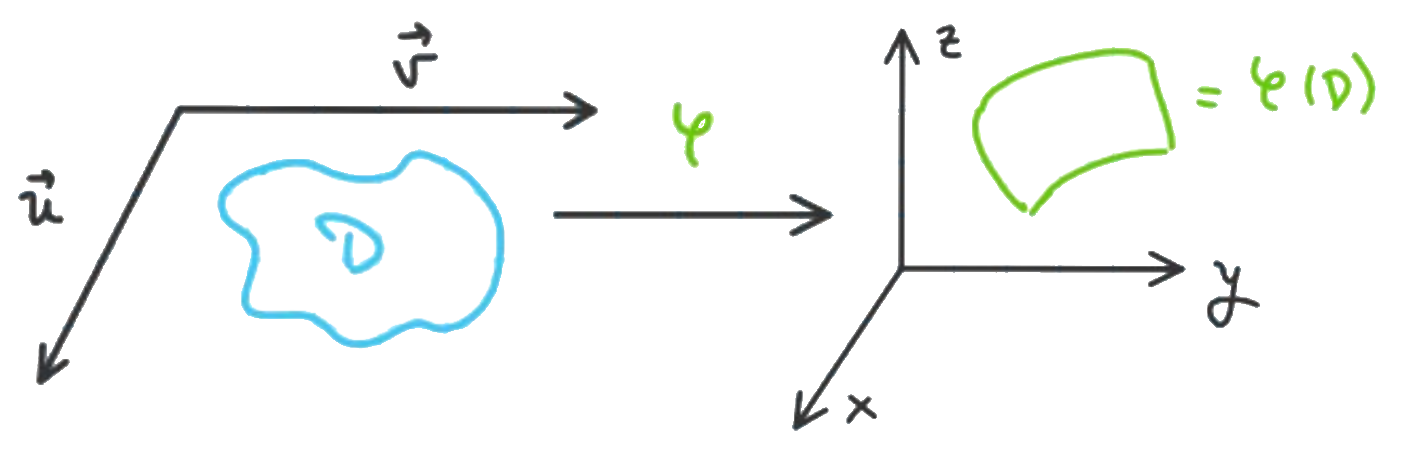
\includegraphics[width=\textwidth]{comentario4.5.1.png}
          }
        \end{wrapfigure}
        Si suponemos que $\varphi$ es difierenciable en $(u_0,v_0)\in\bbR^2$, fijando un cierto $u_0$
        obtenemos una función con imagen una curva en $S = \varphi\left(\mcD\right)$.
        \noindent \begin{align*}
          \hspace*{-1.1cm}f \colon &\bbR \longrightarrow \bbR^3\\
          \hspace*{-1.1cm}& t \longmapsto \varphi(v_0,t)
        \end{align*}

        \noindent Esto nos permite definir un vector tangente: $\vec{T_v}=\frac{\partial x}{\partial v}(u_0,v_0)\hat{x}+
        \frac{\partial y}{\partial v}(u_0,v_0)\hat{y}+\frac{\partial z}{\partial v}(u_0,v_0)\hat{z}$.\\
        
        \noindent Si ahora fijamos $v_0$ en lugar de $u_0$, podemos tener una función $t\longmapsto\varphi(t,v_0)$ y tenemos otra curva
        sobre $S=\varphi\left(\mcD\right)$ y un vector tangente $\vec{T}_u$ \textit{idem} con $\vec{T}_v$.\\
        
        \noindent El hecho de que $\vec{T}_u$ y $\vec{T}_v$ sean tangentes a dos curvas sobre una superficie $S$ en $\phi\left(u_0,v_0\right)$
        entonces determinan un plano tangente a la superficie $S$ en ese punto. El vector $\vec{T}_u \times \vec{T}_v$ es normal al plano 
        generado por $\vec{T}_u$ y $\vec{T}_v$, y entonces es normal a $S$.\\
      }

      \definicion{Superficie suave}{
        Se dice que una superficie $S$ es \textbf{suave} en $\phi\left(u_0,v_0\right)$ si $\vec{T}_u\times\vec{T}_v\neq\vec{0}$ en 
        $\left(u_0,v_0\right)$. Se dice que $S$ es \textbf{suave} si lo es para todos los puntos de la superficie $S$.
      }
      \definicion{Plano tangente}{
        Si una superficie $S$ es suave (i.e. $\ovl{T_u}\times\ovl{T_v}\neq\ovl{0}$)
        definimos \textbf{el plano tangente de $S$} en $\Phi\left(u_0,v_0\right)$ como el plano
        determinado por $\ovl{T_u}$ y $\ovl{T_v}$ y con vector normal $\ovl{n}=\ovl{T_u}\times\ovl{T_v}$\\
        Una ecuación del plano tangente a $S$ en $\left(x_0,y_0,z_0\right)$ es:
        \begin{equation}\label{eq:leaf}
          \left(x-x_0,y-y_0,z-z_0\right)\cdot\ovl{n}=0
        \end{equation}
        con $\ovl{n}$ evaluado en $\left(u_0,v_0\right)$\\Si $\ovl{n}=\left(n_1,n_2,n_3\right)$
        entonces \refeq{eq:leaf} se escribe:
        \begin{equation*}
          n_1\left(x-x_0\right)+n_2\left(y-y_0\right)+n_3\left(z-z_0\right)=0
        \end{equation*}
      }
      \ejemplo{Sea $\Phi\colon\bbR^2\rightarrow\bbR^3$ dada por
        $\begin{cases}\begin{aligned}
          x=u\cos v\\
          y=u\sin v\\
          z=u^2+v^2
        \end{aligned}\end{cases}$ ¿Existe un plano tangente? \\Hallar el plano tangente en $\Phi\left(0,1\right)$
        }{
          $\ovl{T_u}=\cos\left(v\right)\ovl{i}+\sin\left(v\right)\ovl{j}+2u\ovl{k}$\\
          $\ovl{T_v}=-\sin\left(v\right)\ovl{i}+\cos\left(v\right)\ovl{j}+2v\ovl{k}$\\
          El plano tangente en $\Phi\left(u,v\right)$ es el conjunto de vectores que pasen
          por $\Phi\left(u,v\right)$ perpendiculares a $\ovl{T_u}\times\ovl{T_v}$ Tenemos:\\
          $\ovl{T_u}\times\ovl{T_v}\neq\ovl{0}=\setlength\extrarowheight{0pt}\begin{pmatrix}
          -2u^2\cos\left(v\right)+2v\sin\left(v\right)\\-2u^2\sin\left(v\right)-2v\cos\left(
          v\right)\\u\end{pmatrix} \hspace{1.5cm}\ovl{T_u}\times\ovl{T_v}=\ovl{0}\Longleftrightarrow
          \left(u,v\right) = \left(0,0\right)$\\Entonces el plano tangente en $\Phi\left(0,0\right)$
          pero sí en los otros puntos. Por ejemplo en $\Phi\left(0,1\right)=\left(1,0,1\right)$
          tenemos $\ovl{n}=\ovl{T_u}\times\ovl{T_v}=\setlength\extrarowheight{0pt}\begin{pmatrix}
          -2\\0\\1\end{pmatrix}$ así que una ecuación del plano tangente es: $-2\left(x-1\right)
          +\left(z-1\right)=0$ es decir, $z=2x-1$
        }
      \clearpage
    \subsection{Área de una superficie}
      \noindent En esta sección, consideraremos sólo superficies suaves a trozos que sean uniones de imágenes
      de superficies parametrizadas $\Phi_i\colon\mcD_i\longrightarrow\bbR^3$ tales que: (Los 'quizás'
      son a causa de medidas matemáticas que se definen en \textit{Análisis Funcional})
      \begin{enumerate}
        \item $\mcD_i$ es una región elemental del plano.
        \item $\Phi_i$ es de clase $\mcC_1$ y biyectiva, excepto, quizá, en $\partial\mcD$.
        \item La imagen de $\Phi_i$ es suave, excepto, quizá, en un número finito de puntos.
      \end{enumerate}
      \definicion{Área de una superficie}{
        Se define el \textbf{área de una superficie $\mcA\left(S\right)$} de una superficie
        parametrizada por:$$\boxed{\mcA\left(S\right)=\iint_{\mcD}\norm{\ovl{T_u}\times\ovl{T_v}}\ du\ dv}$$
      }
      \comentario{
        En el caso que $S$ fuera unión de superficies $S_i$ su área será la suma de las
        áreas de las $S_i$.
      }
      Entonces tenemos:\\
      $$\mcA\left(A\right)=\iint_\mcD \sqrt{\left(\frac{\partial\left(x,y\right)}{\partial\left(u,v\right)}\right)^2
      +\left(\frac{\partial\left(y,z\right)}{\partial\left(u,v\right)}\right)^2+
      \left(\frac{\partial\left(x,z\right)}{\partial\left(u,v\right)}\right)^2}\ du\ dv
      \hspace{1cm}\text{donde }\frac{\partial\left(x,y\right)}{\partial\left(u,v\right)}=
      \begin{vmatrix}
      \frac{\partial x}{\partial u}& \frac{\partial x}{\partial v}\vspace{2mm}\\
      \frac{\partial y}{\partial u}& \frac{\partial y}{\partial v}
      \end{vmatrix}$$
      \begin{figure}[h]
        \centering
        \vspace{-1mm}
        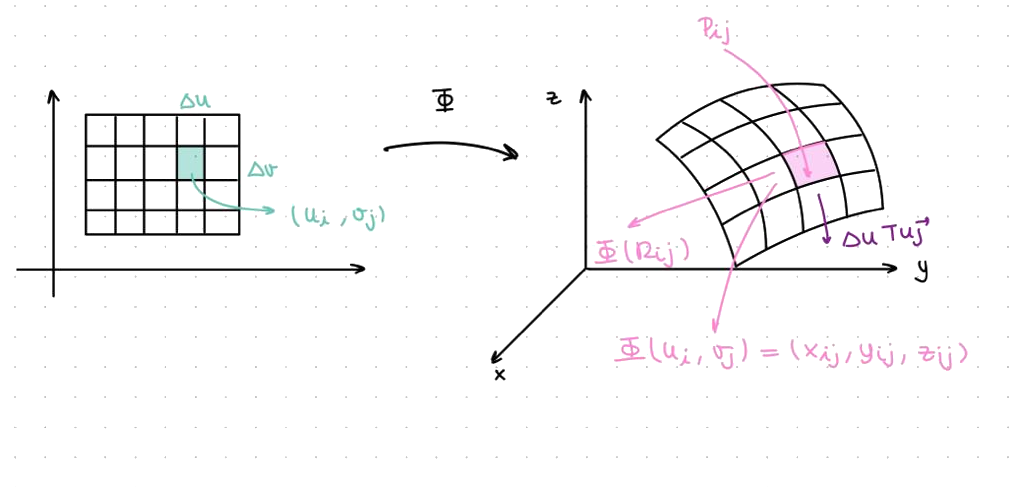
\includegraphics[width=.8\textwidth]{mireia1.png}
      \end{figure}\\
      Hay que considerar una porción de $\mcD$ y sea $R_{ij}$ el ij-ésimo rectángulo
      con vértices $\left(u_i,v_j\right),$$\left(u_{i+1},v_j\right),$$\left(u_i,v_{j+1}\right),$
      $\left(u_{i+1},v_{j+1}\right)$. Los valores de $\ovl{T_u}$ y $\ovl{T_v}$ en $\left(u_i,v_i\right)$
      serán determinados $\ovl{T_{u_i}}$ y $\ovl{T_{v_j}}$. Podemos pensar los vectores
      $\Delta_u\ovl{T_u}$ y $\Delta_v\ovl{T_v}$ como tangentes a la superficie en
      $\Phi\left(u_i,v_j\right)=\left(x_{ij},y_{ij},z_{ij}\right)$ donde $\Delta_u=
      u_{i+1}-u_i$ y $\Delta_v=v_{j+1}-v_j$\\ 

      \noindent Entonces, estos vectores forman un paralelogramo $P_{ij}$ que está en el plano
      tangente a la superficie en $\left(x_{ij},y_{ij},z_{ij}\right)$. Para $n$ grande,
      (es una subdivisión de $n$ trozos), el área de $P_{ij}$ es una buena aproximación
      al área de $\Phi\left(R_{ij}\right)$. Como el area del paralelogramo generado por
      dos vectores $\ovl{v_1}$ y $\ovl{v_2}$ es $\norm{\ovl{v_1}\times\ovl{v_2}}$ entonces
      $\mcA\left(P_{ij}\right)=\norm{\Delta_u\ovl{T_{uj}}\times\Delta_v\ovl{T_{vj}}}=
      \Delta u\Delta v\cdot\norm{\ovl{T_{ui}}\times\ovl{T_{vj}}}$\\ 

      \noindent Por lo tanto, el área total es $\mcA_n=\sum\limits_{i=0}^{n-1}\sum\limits_{j=0}^{n-1}\mcA\left(
      P_{ij}\right)$ y cuando $n\rightarrow\infty$, $\mcA_n\rightarrow\iint_{\mcD}\norm{
      \ovl{T_u}\times\ovl{T_v}}\ du\ dv$
      \ejemplo{
        Sea $\mcD$ la región determinada por $0\leq\theta\leq 2\pi$ y $0\leq r\leq 1$ y
        sea $\Phi\colon\mcD\longrightarrow\bbR^3$ tal que:\vspace{2mm}\\
        Sea la parametrización del cono $S$:
        $\begin{cases}\begin{aligned}
          x=r\cos\theta\\
          y=r\sin\theta\\
          z=r
        \end{aligned}\end{cases}$ hallar su área de superficie.
      }{
        $\frac{\partial\left(x,y\right)}{\partial\left(r,\theta\right)}=
        \begin{vmatrix}
          \cos\theta&   -r\sin\theta\\
          \sin\theta&    r\cos\theta
        \end{vmatrix}=r$\hspace{0.5cm}$\frac{\partial\left(y,z\right)}{\partial\left(r,\theta\right)}
        =-r\cos\theta$ \hspace{0.1cm} y \hspace{0.1cm} $\frac{\partial\left(x,z\right)}{\partial\left(r,\theta\right)}
        =r\sin\theta \implies$\\ \\$\implies\norm{\ovl{T_r}\times\ovl{T_\theta}}=\sqrt{r^2+r^2\cos^2\theta
        +r^2sin^2\theta}=\sqrt{2}r$\\ \\$\mcA=\int_0^2\pi\int_0^1\sqrt{2}r\ dr\ d\theta =\sqrt{2}\pi$
      }
      \comentario{
        Para confirmar que es el area de $\Phi\left(\mcD\right)$ debemos comprobar
        que $\Phi$ es biyectiva para puntos que no están en la frontera de $\Phi$\\
        Sea $\mcD_0$ el conjunto de $\left(r,\theta\right)$ tales que $0<r<1$ y
        $0<\theta <2\pi$ i.e. $\mcD_0 = \mcD\partial\mcD$\\ Para ver que $\Phi$ es
        biyectiva, suponemos que $\Phi\left(r,\theta\right)=\Phi\left(r',\theta'\right)$
        pero $\left(r,\theta\right),\left(r',\theta'\right)\in \mcD_0$\\
        Tenemos:
        \begin{alignat*}{4}
          & \begin{aligned}
            & \begin{cases}\begin{aligned}
              &r\cos\theta=r'\cos\theta'\\
              &r\sin\theta=r'\sin\theta'\\
              &r=r'\\
              \end{aligned}\end{cases}\\
          \end{aligned}
            && \implies \quad &&
          \begin{aligned}
            \begin{cases}\begin{aligned}
              &\cos\theta=\cos\theta'\\
              &\sin\theta=\sin\theta'\\
            \end{aligned}\end{cases} \\
          \end{aligned}
            \quad && \implies\theta=\theta' \text{ ó } \theta=\theta'\left(2\pi\right)
        \end{alignat*}
        \\En conclusión,
        $\begin{cases}\begin{aligned}
          &r=r'\\
          &\theta=\theta'\\
        \end{aligned}\end{cases}$ y eso nos dice que $\Phi$ es biyectiva.\\
      }
      \ejemplo{
        Una helicoide se define como $\Phi\colon\mcD\rightarrow\bbR^3$ con
        $\begin{cases}\begin{aligned}
          x=r\cos\theta\\
          y=r\sin\theta\\
          z=\theta
        \end{aligned}\end{cases}$ y $\mcD$ es la región donde\vspace{-0.5cm}\\ $0\leq\theta\leq 2\pi$ y
        $0\leq r\leq 1$. Hallar su área.
      }{
        \vspace{0.2cm}
        Calculamos $\frac{\partial\left(x,y\right)}{\partial\left(1,0\right)}=r
        \hspace{0.4cm}\frac{\partial\left(y,z\right)}{\partial\left(1,0\right)}=\sin\theta
        \hspace{0.4cm}\frac{\partial\left(x,z\right)}{\partial\left(1,0\right)}=\cos\theta$\\ \\
        $\mcA = \iint_D\norm{\ovl{T_r}\times\ovl{T_\theta}}\ dr\ d\theta=
        \int_{0}^{2\pi}\int_{\theta}^{1}\sqrt{r^2+1}\ dr\ d\theta=\int_{0}^{2\pi}\ d\theta
        \int_{0}^{1}\sqrt{r^2+1}\ dr=\pi\left(\sqrt{2}+\log\left(1+\sqrt{2}\right)\right)$
      }
      \comentario{
        Si consideramos una superficie $\mcS$ dada con $z=f\left(x,y\right)$ donde
        $\left(x,y\right)\in\mcD$ admite la parametrización
        $\begin{cases}\begin{aligned}
          &x=u\\ &y=v\\ &z=f\left(u,v\right)
        \end{aligned}\end{cases}$ con $\left(u,v\right)\in\mcD$. \\ \\
        Si $f$ es de clase $\mcC_1$, entonces la superficie es suave, y el cálculo del
        área se reduce a:$$\boxed{\mcA\left(\mcS\right)=\iint_\mcD\sqrt{1+\left(\frac{\partial f}
        {\partial x}\right)^2+\left(\frac{\partial f}{\partial y}\right)^2}\ dx\ dy}$$
      }
      \clearpage
      \ejemplo{
        Calcular el área de la superficie de la esfera $\mcS$ definida por $x^2+y^2+z^2=1$
        (Indicación: calcular el área del hemisferio superior $\mcS^+$ (i.e. con $z\geq 0$))
      }{
        Tenemos $z=f\left(x,y\right)=\sqrt{1-x^2-y^2}$ con $\left(x^2+y^2\leq 1\right)$
        Sea $\mcD$ la región de $\left(x,y\right)\in\bbR^2/x^2+y^2\leq 1$\\ \\
        $\mcA\left(\mcS^+\right)=\iint_\mcD\sqrt{\frac{x^2}{1-x^2+y^2}+\frac{y^2}{1-x^2-y^2}+1}\ dx\ dy=
        \iint_\mcD\frac{1}{\sqrt{1-x^2-y^2}}\ dx\ dy$\\ \\Aplicamos el
        \textit{Teorema de Fubini}:\\
        $\mcA\left(\mcS^+\right)=\int_{-1}^{1}\int_{-\sqrt{1-x^2}}^{\sqrt{1-x^2}}
        \frac{1}{\sqrt{1-x^2-y^2}}\ dy\ dx=\int_{-1}^{1}\left[\arcsin\left(
        \frac{y}{\left(1-x^2\right)^{\frac{1}{2}}}\right)\right]_{-\sqrt{1-x^2}}^{
        \sqrt{1-x^2}}\ dx=\int_{-1}^{1}\left(\frac{\pi}{2}+\frac{\pi}{2}\right)\ dx=
        2\pi$ \\ \\Por simetría, $\mcA\left(\mcS^-\right)=2\pi$ y finalmente $\mcA\left(
        \mcS^+\right)+\mcA\left(\mcS^-\right)= 4\pi$
      }
  \section{Integrales de funciones escalares sobre superficies}
    \definicion{}{
      Sea $f$ una función continua con valores reales definida en $\mcS$, La integral
      de $f$ sobre $\mcS$ se define: $\iint_{\mcS}f\left(x,y,z\right)\ d\mcS=\iint_\mcS f\ d\mcS$
      (donde $d\mcS$ es un diferencial de superficie)\\ \\
      $\iint_\mcS f\ d\mcS=\iint_{\mcD}f\left(\Phi\left(u,v\right)\right)\norm{\ovl{T_u}
      \times\ovl{T_v}}\ du\ dv$
    }
    \comentario{
      \begin{enumerate}
        \item Si $f\equiv 1$ volvemos a encontrar la fórmula del área
        \item La integral de superficie, como el área de superficie, no depende de la
              parametrización elegida.
        \item Si $\mcS$ es una unión de superficies parametrizadas, si $i=1,\hdots ,N$
              que no se intersecan excepto quizá, a lo largo de curvas que definen sus
              fronteras, entonces: $\iint_\mcS f\ d\mcS=\sum_{i=1}^{N}\iint_{\mcS_i}f\
              d\mcS_i$\\
      \end{enumerate}
    }
    \ejemplo{Consideramos el helicoide $\mcS$ anterior. Sea $f\left(x,y,z\right)=\sqrt{x^2+y^2
    +1}$. Hallar $\iint_\mcS f\ d\mcS$}{
      $\frac{\partial\left(x,y\right)}{\partial\left(r,\theta\right)}=2 \hspace{0.6cm}
      \frac{\partial\left(y,z\right)}{\partial\left(r,\theta\right)}=\sin\theta \hspace{0.6cm}
      \frac{\partial\left(x,z\right)}{\partial\left(r,\theta\right)}=\cos\theta \hspace{1cm}$
      con $r\in[0,1)$, $\theta\in[0,2\pi)$\\ \\
      Tenemos $f\left(r\cos\theta,r\sin\theta,0\right)=\sqrt{r^2+1}$ lo que nos da \\
      $\iint_\mcD f\ d\mcS=\iint_\mcD f\left(\Phi\left(r,\theta\right)\right)\norm{\ovl{T_r}
      \times\ovl{T_\theta}}\ dr\ d\theta= \int_{0}^{2\pi}\int_{0}^{1}\sqrt{r^2+1}\sqrt{r^2+1}\ dr\ d
      \theta=\int_{0}^{2\pi}\frac{4}{3}\ d\theta=\frac{8}{3}\pi$
    }
    \comentario{
      \vspace{-0.25cm}Si $z=g\left(x,y\right)$ con $g\in\mcC_1$ tenemos:\hspace{0.2cm}
      $\boxed{\iint_\mcS f\ d\mcS=\iint_\mcD f\left(x,y,g\left(x,y\right)\right)\sqrt{1+\left(
      \frac{\partial g}{\partial x}\right)^2+\left(\frac{\partial g}{\partial y}\right)^2}
      \ dx\ dy}$
    }
    \ejemplo{Sea $\mcS$ una superficie definida por $z=x^2+y$ donde $\mcD$ es la región
      caracterizada por $0\leq x\leq 1$ y $-1\leq y\leq 1$. Calcular $\iint_\mcD x\ d\mcS$}{
      Tenemos $\iint_\mcS xd\mcS=\iint_\mcD x\sqrt{1+4x^2+1}\ dxdy=\int_{-1}^{1}\left(
      \int_{0}^{1}x\sqrt{4x^2+2}dx\right)dy=\frac{1}{8}\int_{-1}^{1}\left(\int_{0}^{1}
      8x\left(4x^2+2\right)^\frac{1}{2}dx\right)dy=\frac{2}{3}\frac{1}{8}\int_{-1}^{1}
      \left[\left(2+4x^2\right)^\frac{3}{2}\right]_0^1dy=\frac{1}{12}\int_{-1}^{1}\left(
      6^\frac{3}{2}-2^\frac{3}{2}\right)dy=\sqrt{2}\left(\sqrt{3}-\frac{1}{3}\right)$
    }
    \clearpage
    \comentario{
      Si $z=g\left(x,y\right)$\\
      \begin{wrapfigure}{r}{.3\textwidth}
        \vspace{-0.5cm}
        \vspace{-1\intextsep}
        \centering
        \ffigbox[\textwidth]{}{
          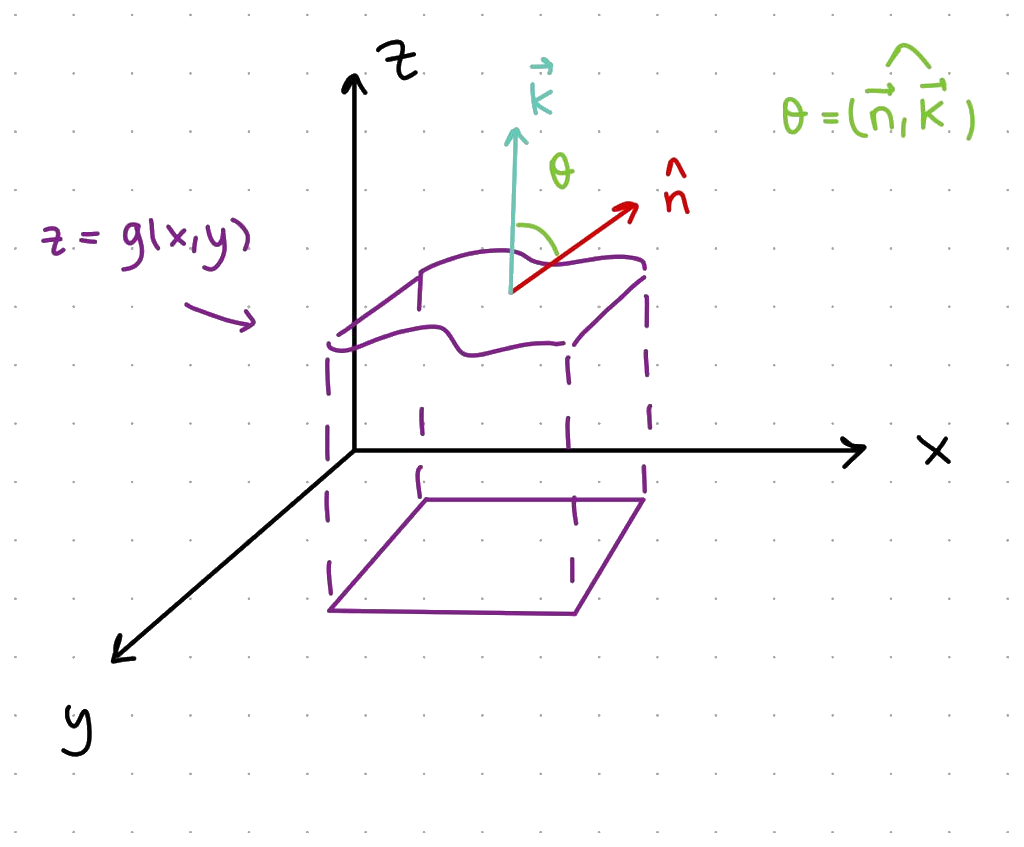
\includegraphics[width=\textwidth]{mireia2.png}
        }
      \end{wrapfigure}
      $\Phi\left(x,y,z\right)=z-g\left(x,y\right)=0$\\
      Un vector normal a $\Phi\text{ es }\ovl{n}=\ovl{\nabla}\Phi$
      $\text{es decir, }\boxed{\ovl{n}=-\frac{\partial g}{\partial x}\ovl{i}-\frac{\partial g}{\partial y}\ovl{j}+\ovl{k}}$
      \vspace{0.2cm}\\$\ovl{n},\ovl{k}=\norm{\ovl{n}}\cdot\norm{\ovl{k}}\cdot
      \cos(\ovl{n},\ovl{k}) \Leftrightarrow\cos\theta=
      \frac{\ovl{n}\cdot\ovl{k}}{\norm{\ovl{n}}\cdot\norm{\ovl{k}}}=
      \frac{\ovl{n}\cdot\ovl{k}}{\norm{\ovl{n}}}=\frac{1}{\norm{\ovl{n}}}
      \Leftrightarrow\norm{\ovl{n}}=\frac{1}{\cos\theta}\\
      \text{(sabiendo que }\ovl{k}\text{ es unitario y es }\left(0,0,1\right)\text{)}\vspace{0.2cm}\\
      \text{Al final obtenemos, } \boxed{\iint_\mcS f\ d\mcS=\iint_\mcD\frac{f\left(x,y,
      g\left(x,y\right)\right)}{\cos\theta}\ dxdy}$
    }

    \ejemplo{Calcular $\iint_\mcS x\ d\mcS$ donde $\mcS$ es el triángulo con vértices
    $\left(1,0,0\right),\left(0,1,0\right),\left(0,0,1\right)$ (indicación: encontrar un
    vector normal $\ovl{n}$ unitario, tendriámos $\ovl{n}\cdot\ovl{k}=\cos\theta$)}{
      Esta superficie es el plano dado por $x+y+z=1$. Un vector normal $\ovl{n}$ a
      este plano tiene coordenadas $\left(1,1,1\right)$. Tenemos $\norm{\ovl{n}}=\sqrt{3}$
      lo que nos da un vector normal unitario a este plano $\ovl{n}=\frac{\ovl{n}}{\norm{\ovl{n}}}
      \left(\frac{1}{\sqrt{3}},\frac{1}{\sqrt{3}},\frac{1}{\sqrt{3}}\right) \text{esto va vertical}$.
      Con la fórmula del comentario anterior, tenemos $\iint_\mcS x\ d\mcS=\iint_\mcD \frac
      {x}{\ovl{n}\cdot\ovl{k}}\ dxdy=\iint_\mcD \frac{x}{\frac{1}{\sqrt{3}}}$ donde
      $\ovl{n}\cdot\ovl{k}=\norm{\ovl{n}}\norm{\ovl{k}}\cos\theta\Leftrightarrow
      \ovl{n}\cdot\ovl{k}=\cos\theta$ porque $\norm{\ovl{n}}\norm{\ovl{k}}=1$ por unitarios.\\
      $\iint_\mcD \frac{x}{\frac{1}{\sqrt{3}}}=\sqrt{3}\int_{0}^{1}\int_{0}^{1-x}x\ dydx=
      \frac{\sqrt{3}}{6}$
    }
  \section{Integrales de superficie de funciones vectoriales}
    \definicion{Superficie orientada}{
      Una superficie suave $\mcS$ es una \textbf{superficie orientada} si existe una función
      normal unitaria $\ovl{n}$ definida en cada punto $\left(x,y,z\right)$ sobre la superficie.
      El campo vectorial $\ovl{n}\left(x,y,z\right)$ recibe el nombre de \textbf{orientación}
      de $\mcS$.\\ \\ Puesto que una normal unitaria a $\mcS$ puede ser $\ovl{n}\left(x,y,z\right)
      $ o $-\ovl{n}\left(x,y,z\right)$, una superficie \textbf{orientada} tiene dos orientaciones.
    }
    \comentario{
      Tenemos $\ovl{n}=\frac{\ovl{T_u}\times\ovl{T_v}}{\norm{\ovl{T_u}\times\ovl{T_v}}}$
      Una superficie $\mcS$ definida por $z=g\left(x,y\right)$ tiene una orientación
      hacia arriba cuando las normales unitarias están dirigidas hacia arriba.
    }
    \definicion{Superficie cerrada}{
      Una superficie \textbf{cerrada} se define como la frontera de un sólido finito.
    }
    \ejemplo{}{La superficie de una esfera es una superficie cerrada}
    \clearpage
    \comentario{
      \begin{enumerate}
        \item Si una superficie \textbf{suave} $\mcS$ está definida por
              $f\left(x,y,z\right)=0$ entonces la normal es \textbf{unitaria} $\ovl{n}=\frac{\ovl{\nabla}f}
              {\norm{\ovl{\nabla}f}}$
        \item Si $f$ está definida de forma explícita, $z=g\left(x,y\right)$ podemos escribir\\
              $f\left(x,y,z\right)=g\left(x,y\right)-z$ o $f\left(x,y,z\right)z-g\left(x,y\right)$
              en función de la orientación.
        \item Si S está definida por $z=g\left(x,y\right)$ hay dos vectores unitarios en 
              $\left(x_0,y_0,g\left(x_0,y_0\right)\right)$.
              $$\vec{n}=\frac{-\frac{\partial g}{\partial x}\left(x_0,y_0\right)\vec{i}-
              \frac{\partial g}{\partial y}\left(x_0,y_0\right)\vec{j}+\vec{k}}
              {\sqrt{\left(\frac{\partial g}{\partial x}\left(x_0,y_0\right)\right)^2+
              \left(\frac{\partial g}{\partial y}\left(x_0,y_0\right)\right)^2+1}} 
              \text{ y $\vec{n}$' en el sentido opuesto.}$$
      \end{enumerate}
    }
    \teorema{}{
      \begin{enumerate}
        \item Sea $S$ una superficie parametrizada y sean $\phi_1$ y $\phi_2$ dos parametrizaciones de $S$ suaves
              y que preserven la orientación (el vector normal que se obtiene va hacia arriba, abajo invierte la orientación).
              $$\iint_{\phi_1}F\ dS=\iint_{\phi_2}F\ dS$$
        \item Si $\phi_1$ preserva la orientación y $\phi_2$ la invierte, entonces
              $$\iint_{\phi_1}F\ dS=-\iint_{\phi_2}F\ dS$$
      \end{enumerate}
    }
    \comentario{
      \begin{enumerate}
        \item Si $f$ es un campo escalar, $\iint_{\phi_1}f\ dS=\iint_{\phi_2}f\ dS$\\
              (la integral no depende de la parametrización).
        \item $\iint_S\vec{F}\cdot d\vec{S}=\iint_S\vec{F}\cdot\left(\vec{T_u}\times\vec{T_v}\right)\ dudv=\iint_D\vec{F}\cdot\frac{\vec{T_u}\times\vec{T_v}}{\norm{\vec{T_u}\times\vec{T_v}}}
              \norm{\vec{T_u}\times\vec{T_v}}\ dudv=\iint_D\vec{F}\cdot\vec{u}\cdot dS$\\

              Donde:

              $d\vec{S}=\left(\vec{T_u}\times\vec{T_v}\right)\ dudv$ es el vector diferencial de superficie\\ 
              $dS = \norm{\vec{T_u}\times\vec{T_v}}\ dudv$ es el diferencial de superficie\\
              $\vec{n}=\dfrac{\vec{T_u}\times\vec{T_v}}{\norm{\vec{T_u}\times\vec{T_v}}}$ es la normal unitaria\\
      \end{enumerate}
    }
    \clearpage
    \section*{Algunas Parametrizaciones}
      \subsection*{Parametrización de una \textbf{elipse}}
      $$\frac{(x-\alpha)^2}{a^2}+\frac{(y-\beta)^2}{b^2}=1\hspace{1cm}  
      \begin{cases}\begin{aligned}
        &x(t)=\alpha+a\cos(t)\\
        &y(t)=\beta+b\sin(t)\\
      \end{aligned}\end{cases}$$
      \subsection*{Parametrización de una \textbf{parábola}}
      \noindent La ecuación canónica de una parábola con vértice $V\left(\alpha,\beta\right)$ y eje horizontal es $\left(y-\beta\right)^2=4c\left(x-\alpha\right)$.\\
      Con eje vertical sería $\left(x-\alpha\right)^2=4c\left(y-\beta\right)$
      $$\begin{cases}
        \begin{aligned}
          &x(t)=\frac{1}{4c}t^2+\alpha\\
          &y(t)=t+\beta
        \end{aligned}
      \end{cases} t\in\bbR$$
      \subsection*{Parametrización de una \textbf{espiral}}
        $$\begin{cases}
          \begin{aligned}
            &x(t)=\cos(t)\\
            &y(t)=\sin(t)\\
            &z(t)=t\\
          \end{aligned}
        \end{cases} t\in[a,b]$$

\chapter{Integrales Triples}
    \section{Introducción}
    \noindent Como lo hicimos con la integral doble, vamos a definir la integral de una función en el
    paralelepípedo (rectángulo). $V=\left[a_1,b_1\right]\times\left[a_2,b_2\right]\times\left[a_3,b_3\right]$.\\
    \noindent Sean $N_1,N_2,N_3$ tres enteros dados:
    $\begin{cases}\begin{aligned}
      \vspace{2pt}
      x_i-x_{i-1}=\frac{b_1-a_1}{N_1}\\
      \vspace{2pt}
      y_j-y_{j-1}=\frac{b_2-a_2}{N_2}\\
      \vspace{2pt}
      z_k-z_{k-1}=\frac{b_3-a_3}{N_3}
    \end{aligned}\end{cases}$\\
    lo que nos da \textbf{paralelepípedos elementales} $w_{ijk}=\left[x_{i-1},x_i\right]\times
    \left[y_{j-1},y_j\right]\times\left[z_{k-1},z_k\right]$
    \definicion{Integral Triple}{
      Sea $\mcI_\mcV\left(f\right)=\sum\limits_{i=1}^{N_1}\sum\limits_{j=1}^{N_2}\sum\limits_{k=1}^{N_3}
      f\left(x_i,y_j,z_k\right)\left(x_i-x_{i-1}\right)\left(y_j-y_{j-1}\right)\left(z_k-z_{k-1}\right)$
      si $N_1,N_2$ y $N_3$ se van al infinito, entonces $\mcI_\mcV\left(f\right)$ admite un
      límite en $\bbR$. Este límite se llama \textbf{Integral Triple} de $f$ en $\mcV$y se escribe:
      $$\mcI=\iiint_\mcV f\left(x,y,z\right)\ dx\ dy\ dz$$
    }
    \comentario{
      Como lo hicimos con la integral doble, la integral triple se puede calcular gracias a
      tres integrales simples.
    }
    \teorema{Cálculo directo}{
      \begin{enumerate}
        \item Si $\mcV$ es de la forma siguiente: $$\mcV = \left\{\left(x,y,z\right)
        \in\bbR^3\colon a\leq x\leq b\colon g­_1(x)\leq y\leq g_2(x)\colon h_1(x,y)\leq z
        \leq h_2(x,y)\right\}$$
        $$\text{y entonces, }\iiint_mcV f\left(x,y,z\right)\ dx\ dy\ dz=
        \int_{a}^{b}\left(\int_{g_1(x)}^{g_2(x)}\left(\int_{h_{1}(x,y)}^{h_2(x,y)}f\left(x,y,z\right)\ dz\right)\ dy\right)\ dx$$

        \item Si $\mcV$ es de la forma siguiente: $$\mcV = \left\{\left(x,y,z\right)
        \in\bbR^3\colon a\leq x\leq b\colon g­_1(x)\leq z\leq g_2(x)\colon h_1(x,z)\leq y
        \leq h_2(x,z)\right\}$$
        $$\text{entonces, }\iiint_mcV f\left(x,y,z\right)\ dx\ dy\ dz=
        \int_{a}^{b}\left(\int_{g_1(x)}^{g_2(x)}\left(\int_{h_{1}(x,z)}^{h_2(x,z)}f\left(x,y,z\right)\ dy\right)\ dz\right)\ dx$$

        \item \textit{Idem.}
      \end{enumerate}
    }
  \section{Cambio de variables}
    \noindent Consideramos $\mcI=\iiint_\mcV f\left(x,y,z\right)\ dx\ dy\ dz$ y supongamos que tenemos
    el cambio de variable siguiente:\\
    \begin{tabular}{l}
      \hspace{-1cm}
      $\begin{cases}\begin{aligned}
        &x=a\left(u,v,w\right)\\
        &y=b\left(u,v,w\right)\\
        &z=c\left(u,v,z\right)
      \end{aligned}\end{cases}$\\
    \end{tabular}
    con $\left(u,v,w\right)\in\Omega\text{ biyección de }\mcV$\\
    Podemos, entonces, definir una nueva función $g$ tal que: $g\left(u,v,w\right)=
    f\left(a\left(u,v,w\right),b\left(u,v,w\right),c\left(u,v,w\right)\right)$ lo que nos
    permite escribir:
    \teorema{}{
      $$\iiint_\mcV f\left(x,y,z\right)\ dx\ dy\ dz=\iiint_\Omega g\left(u,v,w\right)
      \begin{vmatrix}J_g\left(u,v,w\right)\end{vmatrix}\ du\ dv\ dw$$
    }
    \ejemplo{Calcular $\mcI=\iiint_\mcV xyz\left(1-x-y-z\right)\ dx\ dy\ dz$ con $\mcV$
    delimitado por los planos\\ $\begin{cases}\begin{aligned}&x=0\\ &y=0\\ &z=0\\ &x+y+z=1\end{aligned}\end{cases}$ con el cambio de variable propuesto:
    $\begin{cases}\begin{aligned}&x=u\left(1-u\right)\\ &y=uv\left(1-w\right)\\ &z=uvw\end{aligned}\end{cases}$}{
      \begin{wrapfigure}[1]{r}{.3\textwidth}
        \vspace{-1\intextsep}
        \begin{center}
          \ffigbox[\textwidth]{}{
            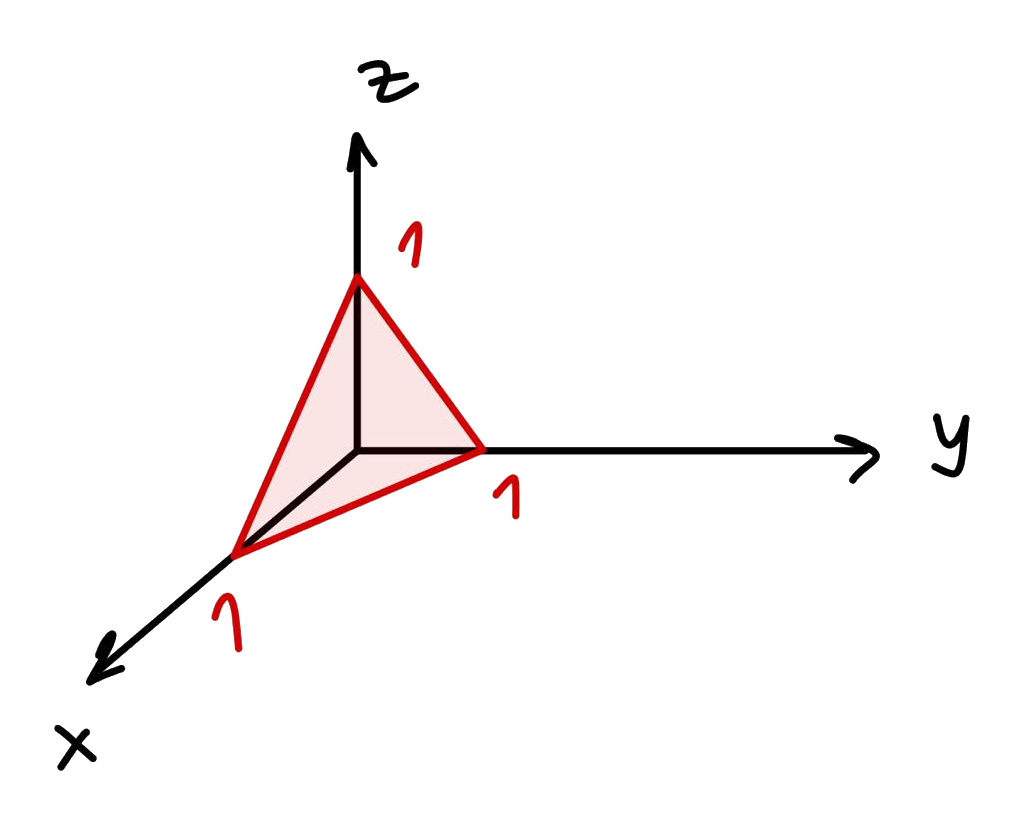
\includegraphics[width=\textwidth]{mireia4.png}
          }
        \end{center}
      \end{wrapfigure}
      Tenemos $g\left(u,v,w\right)=\left(u-uv,uv-uvw,uvw\right)$\vspace{0.4cm}\\
      y además:
      $\begin{cases}\begin{aligned} &u=x+y+z\\ &v=\frac{y+z}{x+y+z}\\ &w=\frac{z}{y+z}\end{aligned}\end{cases}$\vspace{0.4cm}\\
      $\begin{vmatrix}J_g\left(u,v,w\right)\end{vmatrix}=
      \begin{vmatrix}
        1-v&                -u&                 0\\
        v\left(1-w\right)&  u\left(1-w\right)&  -uv\\
        vw&                 uw&                 uv
      \end{vmatrix}=u^2v$\\

      \vspace{0.2cm}$g\left(u,v,w\right)=f\left(u\left(1-v\right),uv\left(1-w\right),uvw\right)=u^3v^2w\left(1-u\right)\left(1-v\right)\left(1-w\right)$\\

      \vspace{0.2cm}$\mcI=\iiint u^5v^3w\left(1-u\right)\left(1-v\right)\left(1-w\right)dudvdw=\int_{0}^{1}u^5\left(1-v\right)dv\int_{0}^{1}w\left(1-w\right)dw=$
      $\left(\frac16-\frac17\right)\left(\frac14-\frac15\right)\left(\frac12-\frac13\right)$
    }
    \subsection{Algunos cambios de variable}
      \subsubsection{Cambio en coordenadas cilíndricas}
        \vspace{0.2cm}
        \begin{wrapfigure}[5]{l}{.27\textwidth}
          \vspace{-0.3cm}
          \vspace{-1\intextsep}
            \begin{center}
              \ffigbox[\textwidth]{}{
                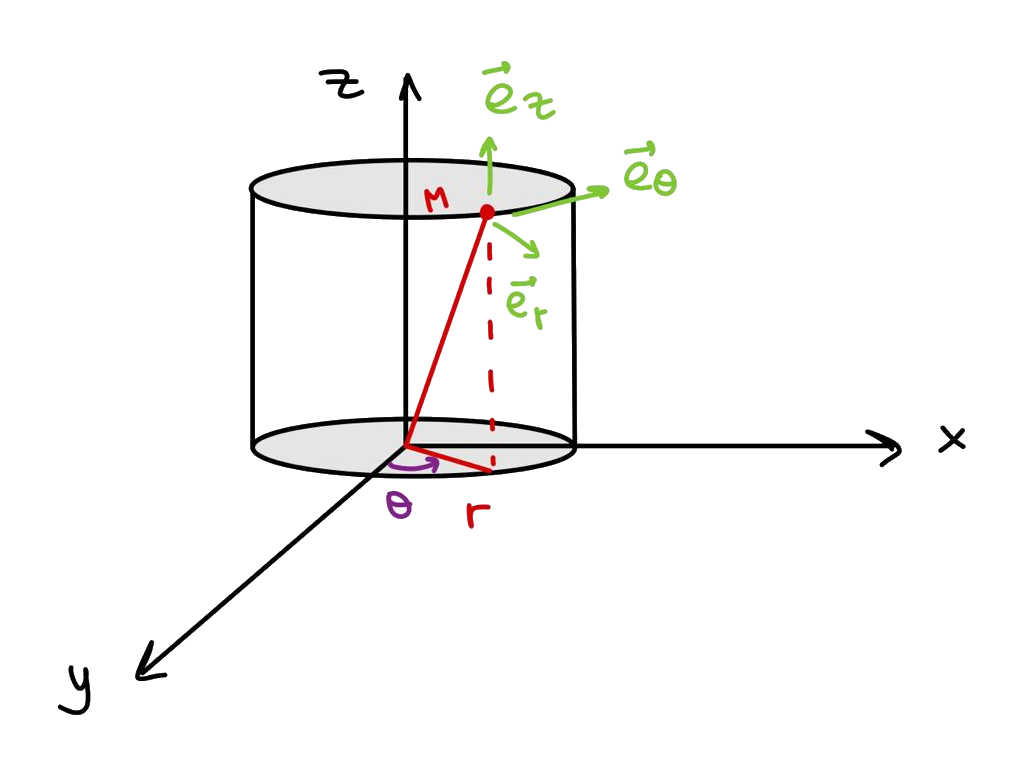
\includegraphics[width=\textwidth]{mireia3.png}
              }
            \end{center}
        \end{wrapfigure}
        $\begin{cases}\begin{aligned} &x=r\cos\theta\\ &y=r\sin\theta\\ &z=z\end{aligned}\end{cases}$ con $r\geq 0,\ \theta\in\left[0,2\pi\right]$
        $\hspace{0.5cm}g\left(r,\theta,z\right)=\left(r\cos\theta,r\sin\theta,z\right)$\\

        \vspace{0.2cm}$\begin{vmatrix}J_g\left(r.\theta,z\right)\end{vmatrix}=
        \begin{vmatrix}\frac{\partial\left(x,y,z\right)}{\partial\left(r,\theta,z\right)}\end{vmatrix}=
        \begin{vmatrix}
        \cos\theta& -r\sin\theta& 0\\
        \sin\theta& r\sin\theta & 0\\
        0         & 0           & 1
        \end{vmatrix}=r$
        $\iiint_V \left(x,y,z\right)\ dx\ dy\ dz=$\vspace{0.4cm}\\
        \hspace*{1cm}$=\iiint_\Omega g\left(r\cos\theta,r\sin\theta,z\right)r\ dr\ d\theta\ dz$

        \clearpage
        \comentario{
          Si $\mcV=\left\{\left(x,y,z\right)\in\bbR^3/(x,y)\in\mcD,\varphi_1(x,y)\leq z \leq\varphi_2(x,Y)\right\}$
          la proyección de $\mcV$ sobre ($Oxy$) es el dominino $\mcD$ tal que:
          $\mcD=\left\{(r,\theta)\in\bbR^2,\alpha<\theta<\beta, h_1(\theta)\leq r \leq h_2(\theta)\right\}$
          Entonces si $f$ es una función continua en $\mcV$ tenemos:
          $$\iiint_\mcV f(x,y,z)dxdydz=\iint_\mcD\left(\int_{\varphi_1(x,y)}^{\varphi_2(x,y)}f(x,y,z)dz\right)dxdy=
          \int_{\alpha}^{\beta}\int_{h_1(\theta)}^{h_1(\theta)}\int_{\varphi_1(x,y)}^{\varphi_2(x,y)}f\left(r\cos\theta,r\sin\theta,z\right)r\ dzdrd\theta$$
        }
        \ejemplo{Calcular $\iiint_\mcV \left(x^2+y^2+1\right)\ dxdydz$\\ donde
        $\mcV=\left\{(x,y,z)\in\bbR^3,x^2+y^2\leq 1\text{ y }0\leq z \leq 2\right\}$}{
          Vamos a utilizar las coordenadas cilíndricas $\begin{cases}\begin{aligned} &x=r\cos\theta\\ &y=r\sin\theta\\ &z=z\end{aligned}\end{cases}$
          e integramos en $\Delta = [0,1]\times[0,2\pi]\times[0,2]$.\\

          \vspace{0.4cm}Tenemos $f(r\cos\theta,r\sin\theta,z)=r^2+1$ lo que nos da $\iiint_\mcV f\left(x,y,z\right)\ dxdydz=
          \iiint_\Delta (1+r^2)r\ drd\theta dz=\int_{0}^{\pi}dz\int_{0}^{2\pi}d\theta\int_{0}^{1}(1+r^2)r\ dr=4\pi\left[\frac{r^2}{2}+\frac{r^4}{4}\right]_0^1
          =4\pi\left(\frac12+\frac14\right)=3\pi$
        }
      \subsection{Coordenadas Esféricas}
        $\begin{cases}\begin{aligned}
          &x = \rho\sin\varphi\cos\theta\\
          &y = \rho\sin\varphi\sin\theta \\
          &z = \rho\cos\varphi\\
          &\rho^2 = x^2+y^2+z^2
        \end{aligned}\end{cases}$ con $\rho\geq 0$, $\theta\in[0,2\pi]$, $\varphi\in[0,\pi]$\\

        \vspace{0.4cm}El Jacobiano será $\boxed{\rho^2\sin\varphi}$
        \comentario{
          Si ponemos
          $\begin{cases}\begin{aligned}
            &r=\rho\sin\varphi\\
            &\theta=\theta\\
            &z=\rho\cos\varphi
          \end{aligned}\end{cases}$ entonces podemos transformar las coordenadas esféricas en cilíndricas $\left(r,\theta,z\right)$
        }
        \ejemplo{Sea $\mcB$ la bola unidad y $a>1$, calcular $\mcI = \iiint_\mcB\frac{dx\ dy\ dz}{\sqrt{x^2+y^2+(z-1)^2}}$}{
          Pasamos a coordenadas esféricas: $\begin{cases}\begin{aligned}
            &x = \rho\sin\varphi\cos\theta\\
            &y = \rho\sin\varphi\sin\theta \\
            &z = \rho\cos\varphi
          \end{aligned}\end{cases}$ y obtenemos\vspace{0.2cm} \\
          $\mcI=\int_{0}^{1}\int_{-\pi}^{\pi}\int_{0}^{2\pi}\frac{\rho^2\sin\varphi}{\sqrt{\rho^2+r^2-2a\rho\cos\varphi}}d\varphi d\theta d\rho$
          \hspace{0.5cm}Hacemos el cambio de variable:
          $\begin{cases}\begin{aligned} &t=\rho^2+a^2-2a\rho\cos\varphi\\ &dt=2a\rho\sin\varphi\ d\varphi\end{aligned}\end{cases}$

          \vspace{0.4cm}y \hspace{0.5cm}$\mcI = 2\pi\int_{0}^{1}\rho^2\left(\int_{(a-\rho)^2}^{(a+\rho)^2}\frac{dt}{2a\rho\sqrt{t}}\right)d\rho = \frac{4\pi}{a}\int_{0}^{1}\rho^2\ d\rho=\frac{4\pi}{3a}$
        }

\chapter{Teoremas de Stokes y Gauss}   
  \vspace{-0.8cm}
  \section{Teorema de Kelvin-Stokes}
    \noindent Empezando por algunas aplicaciones en física, la idea en el campo de mecánica de fluidos es la de observar que las rotaciones en una superficie se superponen entre ellas hasta llegar a la frontera,
    es decir, a partir de lo que ocurre en el interior de la superficie podemos tener una idea de lo que está pasando en la frontera.\\

    \noindent Se trata de gereralizar a $\bbR^3$ el concepto que vimos con el \textit{Teorema de Green-Riemann}. En efecto, si recordamos:\\
    $\vec{F}(x,y)=P(x,y)\vec{i}+Q(x,y)\vec{j}\implies\nabla\times\vec{F}=\left(\frac{\partial Q}{\partial x}(x,y)\vec{i}-\frac{\partial P}{\partial y}(x,y)\vec{j}\right)k$\\
    lo que nos daba $\oint F\ dl=\iint\left(\frac{\partial Q}{\partial x}-\frac{\partial P}{\partial y}\right)\ dS=\iint \nabla\times\vec{F}\cdot\vec{k}dS$\\

    \begin{wrapfigure}[7]{l}{.3\textwidth}
      \vspace{-0.6cm}
      \ffigbox[\textwidth]{}{
        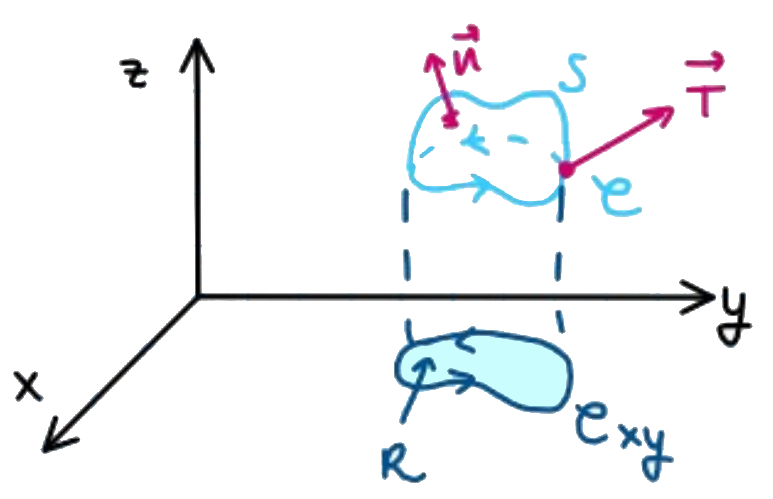
\includegraphics[width=\textwidth]{stokes.png}}
    \end{wrapfigure}

    \noindent El \textit{Teorema de Green-Riemann} en un espacio tridimensional relaciona una integral de línea alrededor de una curva $\mcC$ cerrada, simple, suave (por partes)
    de forma que la frontera de una superficie $S$ con una integral de superficie sobre $S$, como vemos en la figura.
      
    \vspace{0.34cm}\noindent Suponemos que $z=f(x,y)$ es continua cuya representación gráfica es una superficie orientada suave por partes sobre una región $R$ en el plano $OXY$, donde $\mcC$ es la frontera de $S$ y $\mcC_{xy}$ es la frontera de $R$.

    \teorema{\textbf{Kelvin-Stokes}}{
      Sea $S$ una superficie orientada suave por partes y acotada por una curva $\mcC$ cerrada, simple y suave por partes.\\

      Sea $\vec{F}(x,y,z)=P(x,y,z)\vec{i}+Q(x,y,z)\vec{j}+R(x,y,z)\vec{k}$ un cnampo vectorial cuyas componentes son funciones continuas y que tienen derivadas parciales continuas de primer orden en una región abierta de $\bbR^3$ que contiene a $S$.\\

      Si $\mcC$ se recorre en el sentido positivo:
      $$\int_{\mcC}\vec{F}\ dl=\iint_S\nabla\times\vec{F}\cdot d\vec{S}$$
    }
    \clearpage
    \ejemplo{Evaluar $\int_{\mcC}\left(z\ dx+x\ dy+y\ dz\right)$ donde $\mcC$ es la traza del cilindro $x^2+y^2=1$ en el plano $y+z=2$. $\mcC$ está orientado en el sentido contrario al de las manecillas del reloj cuando se mira desde arriba.}{
      Tenemos $\vec{F}(x,y,z)=z\ dx+x\ dy+y\ dz$. Si calculamos $\nabla\times\vec{F}$:\\
      
      \begin{wrapfigure}[3]{l}{.26\textwidth}
        \vspace{-1cm}
        \ffigbox[\textwidth]{}{
          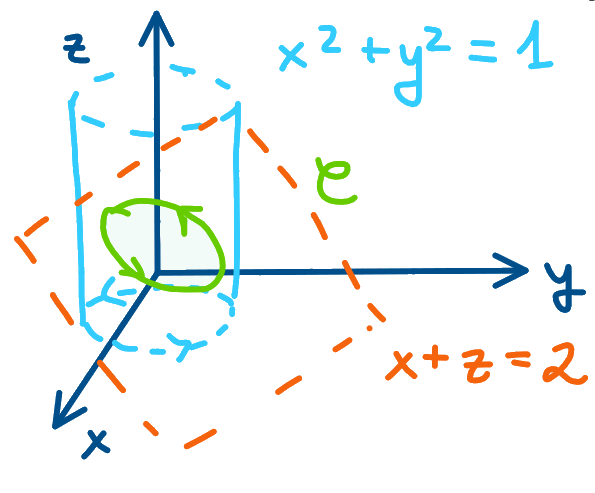
\includegraphics[width=\textwidth]{ejemploStokes.png}}
      \end{wrapfigure}
      \vspace{0.2cm}$\nabla\times\vec{F}=$
      $\begin{vmatrix*}[l]
        \vec{i}                    & \vec{j}                    & \vec{k}\\
        \frac{\partial}{\partial x}& \frac{\partial}{\partial y}& \frac{\partial}{\partial z}\\
        z                          & y                          & z
      \end{vmatrix*} = 1\vec{i}+1\vec{j}+1\vec{k}$

      \vspace{0.4cm}Si $h(x,y,z)=y+z-2$, entonces $h(x,y,z)=0$ es la ecuación del plano cuyo vector normal unitario $\vec{n}=\frac{\nabla h}{\norm{\nabla h}}=\frac{\sqrt{2}}{2}\vec{j}+\frac{\sqrt{2}}{2}\vec{k}$
      
      \vspace{0.6cm}Con el \textit{Teorema de Stokes} tenemos:
      $$\int_{\mcC}\vec{F}d\vec{M}=\iint_{\mcS}\left(\vec{i}+\vec{j}+\vec{k}\right)\cdot\left(\frac{\sqrt{2}}{2}\vec{j}+\frac{\sqrt{2}}{2}\vec{k}\right)\ dS=
      \sqrt{2}\iint_S dS=\sqrt{2}\iint_S \sqrt{2}\ dxdy=2\pi$$
    }
    \comentario{
      Podemos tener:

      \centering
      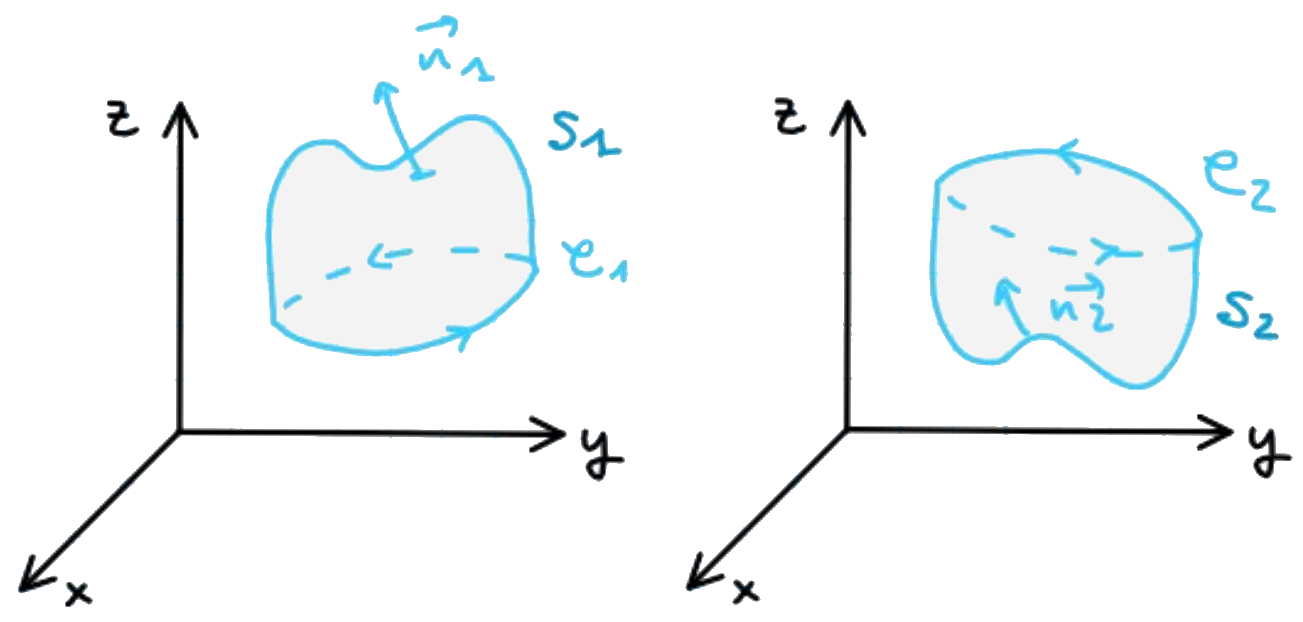
\includegraphics[width=0.5\textwidth]{stokes2.png}
      
      \begin{flushleft} 
      El valor de la integral de superficie está determinado por la integral alrededor de su frontera $\mcC$. Esto significa que la "forma" de la superficie $S$ no tiene importancia:
      $$\int_\mcC\vec{F}\cdot dM=\iint_{S_1}\nabla\times\vec{F}\cdot dS_1=\iint_{S_2}\nabla\times\vec{F}\cdot dS_2$$
      \end{flushleft}
    }
    \comentario{
      En el diagrama siguiente resumimos los resultados para campos conservativos definidos en regiones abiertas conexas y simplemente conexas.
      
      \setlength{\tabcolsep}{2pt}
      \begin{table}[H]
        \begin{tabular}{ccl}
          $\vec{F}\text{ conservativo en }\mcD$ & $\Longleftrightarrow$             & $\vec{F}=\nabla f \text{ en }\mcD$          \\
          \multicolumn{1}{c}{$\Updownarrow$}    & \multicolumn{1}{l}{}              & \multicolumn{1}{c}{$\Updownarrow$}          \\
          $\int_\mcC \vec{F}\cdot d\vec{M}= 0$  & $\xLeftarrow[Stokes]{}$ & $\nabla\cdot\vec{F}=\vec{0}\text{ en }\mcD$
        \end{tabular}
      \end{table}
    }
  \clearpage
  \section{Teorema de Gauss-Ostrogradsky / Divergencia}
    \noindent Si consideramos el punto $(x_0,y_0,z_0)$ como una región infinitesimal de un volumen de control de un gas, entonces podemos entender la divergencia en dicho punto como la medida de cuánto diverge
    o se escapa el gas en dicho punto. Si $\nabla \cdot F>0$, entonces el gas se expande, si $\nabla\cdot F<0$ entonces se contrae, y si $\nabla \cdot F=0$ se dice que el gas es incompresible.\\

    \noindent Se considera un recipiente con un líquido y una membrana semipermeable en su interior. El \textit{Teorema de Gauss-Ostrogradsky} sugiere que para medir cuánto flujo se escapa a través de la membrana
    se puede medir el flujo infinitesimal que se escapa a través de cada punto que la membrana encierra y sumar todos esos puntos. La suma de cada uno de estos flujos infinitesimales que escapan representa
    el flujo total que se escapa de la membrana.

    \teorema{Gauss-Ostrogradsky o \textbf{de la divergencia}}{
      Sea $\Omega$ una región de $\bbR^3$ y sea $S$ la frontera de $\Omega$ con una parametrización $f\colon\mcD\subset\bbR^2\longrightarrow\bbR^3$ que orienta a la superficie con sus vectores normales apuntando
      hacia el exterior.\\

      Si $F(\mcU)\subset\bbR^3\longrightarrow\bbR^3$, $F=(P,Q,R)$ campo vectorial de $\bbR^3$ de clase $\mcC_1$ definido en todo punto del abierto $\mcU$ tal que $\Omega\subseteq\mcU$, entonces:
      $$\iint_S\vec{F}\cdot d\vec{S}=\iiint_\Omega\nabla\cdot\vec{F}\ dV$$
    }
\end{document}

